\documentclass[a4paper]{article}

%% Language and font encodings
\usepackage[english]{babel}
\usepackage[utf8x]{inputenc}
\usepackage[T1]{fontenc}
\usepackage{amssymb}

%% Sets page size and margins
\usepackage[a4paper,top=3cm,bottom=2cm,left=3cm,right=3cm,marginparwidth=1.75cm]{geometry}

%% Useful packages
\usepackage{amsmath}
\usepackage{graphicx}
\usepackage[colorinlistoftodos]{todonotes}
\usepackage[colorlinks=true, allcolors=blue]{hyperref}
\usepackage{stmaryrd}
\usepackage{subfig}
\usepackage{mathtools}
\usepackage{xcolor}
\usepackage{floatrow}
%\usepackage{minted}
\usepackage{verbatim}
\usepackage{fancyvrb}
\usepackage{color}
\usepackage{multicol}
\usepackage{xcolor}

%%%%%%%%%%%%%%%%%%%%%%%%%%%%%%%%%%%%%%%%%%%%%%%%%%%%%%%%%%%%%%%%%%%%%%%%%%%%%%

%% Custom definitions
\DeclarePairedDelimiter\ceil{\lceil}{\rceil}
\DeclarePairedDelimiter\floor{\lfloor}{\rfloor}
\DeclareMathOperator*{\E}{\mathbb{E}}
\newcommand{\R}{\mathbb{R}}
\newcommand{\simtext}[1]{\ensuremath{\stackrel{\text{#1}}{\sim}}}
\newcommand\myeq{\stackrel{\mathclap{\normalfont\mbox{D}}}{=}}
\newtheorem{thm}{Hypothesis}
\newtheorem{lem}[thm]{Result}

\definecolor{bg}{rgb}{0.98,0.98,0.98}
\floatsetup[listing]{capposition=bottom}    

\def\boxitem#1{\setbox0=\vbox{#1}{\centering\makebox[0pt]{%
  \fboxrule=2pt\color{mLightBrown}\fbox{\hspace{\leftmargini}\color{black}\box0}}\par}}

\newenvironment{longlisting}{\captionsetup{type=listing}}{}

\setlength{\columnsep}{0.2cm}

\newcommand{\RomNum}[1]
    {\MakeUppercase{\romannumeral #1}}

\def\boxitem#1{\setbox0=\vbox{#1}{\centering\makebox[0pt]{%
  \fboxrule=2pt\color{mLightBrown}\fbox{\hspace{\leftmargini}\color{black}\box0}}\par}}

\newcommand\dangersign{%
 \makebox[1.8em][c]{%
 \makebox[0pt][c]{\raisebox{.15em}{\small!}}%
 \makebox[0pt][c]{\color{red}\Large$\triangle$}}}%

\newcommand\blfootnote[1]{%
  \begingroup
  \renewcommand\thefootnote{}\footnote{#1}%
  \addtocounter{footnote}{-1}%
  \endgroup
}

\linespread{1.5}

%%%%%%%%%%%%%%%%%%%%%%%%%%%%%%%%%%%%%%%%%%%%%%%%%%%%%%%%%%%%%%%%%%%%%%%%%%%%%%

\title{%
  \large Wiederholung, Ergänzung, Erklärung \& Intuition:\\
  \Large Statistik I \& II für Studierende der Wirtschaftswissenschaften\\
  \large (Ludwig-Maximilians-Universität München)
}
\date{\textbf{Stand:} \today}
\author{\textbf{Autoren:}\\ 
Matthias Aßenmacher\thanks{Institut für Statistik, LMU München; Kontakt bei Fragen \& Anregungen: \url{matthias@stat.uni-muenchen.de}}\qquad
Ann-Kathrin Köpple\thanks{Studentische Hilfskraft (SoSe20), Institut für Statistik, LMU München}\qquad
Christoph Luther\thanks{Studentische Hilfskraft (WiSe 18/19 - SoSe 20), Institut für Statistik, LMU München}\\
Patricia Haro\thanks{Studentische Hilfskraft (WiSe 18/19 - WiSe 19/20), Institut für Statistik, LMU München}\qquad
Maximilian Mandl\thanks{Institut für medizinische Informationsverarbeitung, Biometrie und Epidemiologie, LMU München\vspace{.25cm}}}

%%%%%%%%%%%%%%%%%%%%%%%%%%%%%%%%%%%%%%%%%%%%%%%%%%%%%%%%%%%%%%%%%%%%%%%%%%%%%%

\begin{document}

\maketitle

\blfootnote{
\hspace{-0.75cm} 
\textit{\small 
This work is licensed under a Attribution-NonCommercial 4.0 International (CC BY-NC 4.0)\\          
License details: \url{https://creativecommons.org/licenses/by-nc/4.0/}}
}

\noindent Dieses  Dokument wurde aus verschiedenen Quellen erstellt. Es soll als kleine Verständnishilfe für Studierende angesehen werden, wobei auf mathematische Genauigkeit und Vollständigkeit explizit verzichtet wird. Außerdem wird jedes Thema durch einen Block an Multiple-Choice Aufgaben und Hinweisen auf die passenden \texttt{R}-Funktionen für die behandelten Methoden ergänzt. Für Fehler wird keine Haftung übernommen.\\

\noindent Der erste Teil dieses Dokuments ($\widehat \approx$ Statistik I) wurde von Ann-Kathrin in Zusammenarbeit mit Matthias im Sommer 2020 verfasst. Ann-Kathrin verantwortete das Schreiben des Erstentwurfs, Matthias war verantwortlich für intensives Korrekturlesen, Anpassungen und Erweiterungen.\\
Der zweite Teil ($\widehat \approx$ Statistik II) basiert auf Vorlesungszusammenfassungen von Max aus dem Sommer 2019, welche in Zusammenarbeit mit Christoph, Patricia \& Matthias in dieses Format gegossen und detaillierter ausgearbeitet wurden. Besonderer Dank für diesen zweiten Teil gilt Herrn Dr. Alexander Engelhardt, der freundlicherweise einen Teil seines Materials zur Verfügung gestellt hat (siehe auch: \url{https://www.crashkurs-statistik.de}), sodass wir uns hiervon inspirieren lassen konnten. Aufgrund des Fehlens der Themenbereiche Kombinatorik, Wahrscheinlichkeitsrechnung \& Multiple Regression wurden diese im Sommer 2020 von Ann-Kathrin \& Matthias ergänzt.

\clearpage

\tableofcontents

\clearpage

\hspace{0pt}
\vfill
\begin{center}
    {\Huge Statistik I}
\end{center}
\vfill
\hspace{0pt}

\clearpage

%%%%%%%%%%%%%%%%%%%%%%%%%%%%%%%%%%%%%
%%%%%%%%%%  KAPITEL 1
%%%%%%%%%%%%%%%%%%%%%%%%%%%%%%%%%%%%%

\section{Grundbegriffe, Skalenniveaus, Datenerhebung}

\subsection{Was ist die Statistik?}

Die Statistik kann man in drei verschiedene Grundaufgaben einteilen. Die deskriptive, explorative und induktive Statistik. In Statistik I wird hauptsächlich die deskriptive und die explorative Statistik thematisiert.
\begin{itemize}
     \item Deskriptive Statistik: Das Ziel der deskriptiven Statistik ist es, umfangreiches Datenmaterial in Tabellen, Graphiken und Kennzahlen übersichtlich darzustellen. Viele dieser Methoden sind bereits aus der Schule bekannt (z.B. Kreis- und Balkendiagramm oder arithmetisches Mittel a.k.a. der Durchschnitt) und werden in dieser Veranstaltung durch weitere Ma\ss{}zahlen und Darstellungsweisen erg\"anzt.
     \item Explorative Statistik: Hierbei wird das aufbereitete Datenmaterial auf Strukturen und Muster untersucht um mögliche Hypothesen aufzustellen.
\end{itemize}

\noindent Der Begriff \textit{Daten} mag f\"ur den ein oder anderen etwas neu sein, bezeichnet jedoch im Grunde genommen nichts anderes als eine Messung oder Erhebung von Werten. Vereinfachend kann man sich einen \textit{Datensatz} z.B. einfach als die Messung der Gr\"o\ss{}e aller Personen im H\"orsaal vorstellen.

\subsection{Grundbegriffe}
\subsubsection{Untersuchungseinheit und Grundgesamtheit}
Die \textbf{Untersuchungseinheit} ist ein einzelnes zu untersuchendes Objekt, welches durch das Symbol $\omega$ dargestellt wird.
\\Die \textbf{Grundgesamtheit} ist die Menge an Objekten, über die man etwas sagen möchte. Das Symbol der Grundgesamtheit ist $\Omega$. Somit sind alle Untersuchungseinheiten zusammen die Grundgesamtheit. Diese Beziehung lässt sich wie folgt umschreiben: $\omega \in \Omega$
\\ \textbf{Beispiel:} Die gesamten Studenten im H\"orsaal sind die Grundgesamtheit. Ein einzelner Student ist die Untersuchungseinheit.

\subsubsection{Bestandsmasse und Bewegungsmasse}
 Wenn man die Grundgesamtheit $\Omega$ zu einem bestimmten Zeitpunkt einmal misst, dann spricht man von einer \textbf{Bestandsmasse}.\\
 Beispiel hierfür ist die Messung, bei der festgestellt wird wie viele Studenten am Semesteranfang (10. Oktober) immatrikuliert sind.\\
Im Gegensatz dazu spricht man von einer \textbf{Bewegungsmasse} wenn Ereignisse gemessen werden, die über einen bestimmten Zeitraum eintreten können. Das wären zum Beispiel die Studenten, die während des Wintersemesters das Studium abbrechen.

\subsubsection{Merkmale und Merkmalsausprägungen}
Wenn wir von einer bestimmten Eigenschaft oder einem Aspekt der Untersuchungseinheit sprechen, nennt man dies \textbf{Merkmal} oder \textbf{statistische Variable}.
\\Wenn man sich nun für einen gemessenen/konkreten Wert eines Merkmals interessiert, dann nennt man das \textbf{Merkmalsausprägung}.
In unserem \textbf{Beispiel} könnte man sich für die Leistung in Statistik I der Studenten interessieren, somit sind die \textbf{Merkmalstr\"ager} \textit{Studenten, die Statistik I belegt haben}.
Eine konkrete \textbf{Merkmalsausprägung} mit dem \textbf{Merkmal}: "\textit{Leistung in Statistik I}"  wäre dann auf der Notenskala 1,0 bis 5,0 beispielsweise die Note 2,3.\\
Es gibt zwei Arten von Merkmalsausprägungen:
\begin{itemize}
     \item \textbf{Qualitative:}  Merkmalsausprägungen, sind Ausprägungen, die keinen mathematischen Wert annehmen, also nicht aus Zahlen bestehen. In unserem Beispiel wäre das z.B. die Einteilung der Leistungen in \textit{bestanden} und \textit{nicht bestanden}.
    \item \textbf{Quantitativ:} Merkmalsausprägungen sind \textit{messbar} und werden somit mit Zahlen angegeben. Beispielsweise in der Klausur 40 von 60 Punkten erreicht.
    Quantitative Merkmalsausprägungen kann man weiter unterscheiden in diskret, stetig und quasistetig.
    \begin{itemize}
        \item \textbf {Diskrete} Merkmale haben abz\"ahlbar viele m\"ogliche Merkmalsauspr\"agungen, das heißt nicht quasi unendlich viele Ausprägungen wie z.B. Sandkörner am Meer (mehr dazu s.u. bei \textit{quasistetig}), sondern man kann die möglichen Merkmalsausprägungen mit nicht allzu großem Aufwand abzählen.
        (Bsp.: Geschlecht (da gibt es nur männlich oder weiblich) oder die Platzierung beim Schönheitswettbewerb (bei einer Teilnahme von 5 Personen, kann ich nur Platz 1, 2, 3, 4 oder 5 bekommen), Studiendauer in Semestern)
        \item\textbf{Stetige} Merkmale können unendlich viele verschiedene Merkmalsausprägungen haben. (Das Alter, da zwischen bspw. 18 und 19 unendlich viele Nachkommastellen vorhanden sein können, oder aber auch Anteilswerte sind hierfür ein gutes Beispiel) 
        \item \textbf{Quasistetigen} Daten sind theoretisch stetig (bspw. Körpergröße, Gewicht, o.ä.) Daten, werden aber nur auf einer diskreten Skala (in sehr kleinen Einheiten) gemessen. Da solche Daten \textit{praktisch} in den meisten Fällen auch wie stetige Daten behandelt werden, spricht man hier von \textit{quasistetigen} Daten.
        \item Werden (quasi)stetige Daten in Klassen eingeteilt (bspw. Abfrage von Gehalt in Fragebögen), so spricht man von \textbf{klassierten} oder \textbf{klassiert-stetigen} Daten. Diese Klassenbildung hat weitreichende Implikationen für die anwendbaren Methoden (vgl. folgende Kapitel).
    \end{itemize}
\end{itemize}
Der \textbf{Merkmalsraum} oder \textbf{Zustandsraum} ist die Menge aller möglichen Merkmalsausprägungen. Hier in unserem Beispiel hat der Merkmalsraum des Merkmals Notenleistung gerundet auf ganze Noten eine M\"achtigkeit von 5 (Die Noten: 1, 2, 3, 4, 5)

\subsubsection{Skalentypen}\label{sec:Skalentypen}
Merkmale besitzen aufgrund der Eigenschaften ihrer m\"oglichen Merkmalsausprägungen bestimmte Skalierungen. Diese richtig zuordnen zu können ist sehr wichtig, denn je nach Skalentyp kann man in den folgenden Kapiteln unterschiedliche Maßzahlen bestimmen. 

\paragraph{Nominalskala:} Die Ausprägungen bei einer Nominalskala können nur voneinander unterschieden werden, jedoch nicht geordnet oder ins Verhältnis gesetzt werden. Daher kann man die Merkmalsausprägungen nicht werten, in dem man bspw. sagt, blaue Autos seien besser als (oder doppelt so gut wie) rote Auto. 
Die einzige Aussage die getroffen werden kann ist, ob die Ausprägungen \textit{gleich oder ungleich} sind.

\paragraph{Ordinalskala:} Bei der Ordinalskala können wir nicht nur eine Aussage über gleich/ungleich (wie bei der Nominalskala) treffen, sondern zusätzlich auch die Ordnung, d.h. über \textit{kleiner und größer}. Somit können ordinale Merkmale in eine natürliche Rangfolge/Ordnung gebracht werden. Diese Ordnung kann interpretiert werden, jedoch nicht die Abstände. Beispiele hierfür wären die Schweregrade eines Computerspiels oder die Güteklassen eines Hotels, da man zwar sagen kann, dass das 4-Sterne-Hotel besser als das 2-Sterne-Hotel ist, nicht jedoch, dass es doppelt so gut ist o.\"a. 

\paragraph{Metrische Skala:} Die metrische Skala besitzt den höchsten Informationsgehalt. Denn hier kann man zusätzlich zu den Aussagen gleich/ungleich und größer/kleiner auch Aussagen über Abstände zwischen den Merkmalsausprägungen treffen. Somit kann man die Merkmalsausprägungen in eine Ordnung bringen und die Abstände zwischen den Merkmalsausprägungen messen und interpretieren. Die metrische Skala kann man weiter auf splitten in Intervall- und Verhältnisskala:\\
\noindent Bei der \textbf{Intervallskala} können Differenzen gebildet werden um eine Aussage über den Abstand zu machen, jedoch keine Quotienten, da es kein (natürlichen) Nullpunkt gibt um zwei Werte in Relation zu einander zu setzen. (\textbf{Beispiel} Temperatur: Man kann sagen, dass es heute 10 Grad kälter als gestern ist, jedoch nicht , dass es heute halb so warm ist wie gestern.\\
Bei der \textbf{Verhältnisskala} gibt es diesen natürlichen Nullpunkt. Deshalb kann man Quotienten bilden und Verhältnisse sinnvoll interpretieren. (\textbf{Beispiel} Größe: Man kann sagen, dass Person A doppelt so gro\ss{} ist wie Person B.)
Ein Spezialfall der Verhältnisskala ist die Absolutskala, da nur natürliche Einheiten vorkommen (keine physikalischen Größen). \textit{Nat\"urliche Einheiten} sind bspw. Anzahlen, im Sinne von 10 Äpfel oder 5 Blumen.

\subsection{Datenerhebung}
Um mit Daten arbeiten zu können müssen diese erst einmal "entstehen oder hergestellt" werden. Dafür gibt es die Datenerhebung. Diese \textit{beschafft} Informationen bzw. \textit{gewinnt} Daten.

\subsubsection{Erhebungsarten}

\textbf{Primärerhebung:} Wenn ich selbst eine Erhebung (Befragung, Beobachtung, Experiment) starte ohne auf vorhandenes Material zurück zu greifen, dann wird es als Primärerhebung bezeichnet.\\
\textbf{Sekundärerhebung}: Wenn ich auf bereits vorhandenes Material zurückgreife (z.B. Daten/Statistiken aus dem Internet) dann handelt e sich um eine Sekundärerhebung. Das Material existierte schon vor meiner Recherche.

\subsubsection{Umfang}
Bei Erhebungen, kann man entweder alle Untersuchungseinheiten einer Grundgesamtheit miteinbeziehen, dann spricht man von einer \textbf{Voll-/Totalerhebung} oder nur eine Teilmenge der Grundgesamtheit miteinbeziehen. Dann spricht man von einer \textbf{Teilerhebung (Stichprobe)}.
Ein Beispiel für die Totalerhebung wäre eine Volkszählung oder eine Evaluation, bei der alle Studenten befragt werden.\\
Teilerhebungen sind zum Beispiel Qualitätsprüfungen von Produkten, bei denen einzelne Produkte überprüft werden oder die Sonntagsumfrage bei der einzelne, zufällig ausgewählte Bürger aus der Bevölkerung abstimmen können, wen sie wählen würden wenn aktuell Bundestagswahl wäre.

\subsubsection{Datenform}
Je nachdem wie oft und über welchen Zeitraum eine Erhebung gemacht wird, gibt es bestimmte Datenformen.
Bei \textbf{Querschnittsdaten} wird der Ist-Zustand zu einem bestimmten Zeitpunkt aufgenommen. An mehreren Untersuchungseinheiten werden ein oder mehrere Merkmale nur \textit{einmal} erhoben. \textbf{Beispiele} hierfür sind Lehrerevaluationen oder der Mietspiegel.\\
Eine Erweiterung hiervon sind die \textbf{Longitudinal-, Längsschnitt,- oder Paneldaten}. Hierbei werden ein oder mehrere Merkmale an mehreren Untersuchungseinheiten zu \textit{verschiedenen} Zeitpunkten wiederholt erhoben. Somit interessiert uns hier u.a. auch die Entwicklung der Merkmale im Zeitverlauf.\\
\textbf{Beispiele:} SOEP (Wiederholungsbefragung von privaten Haushalten in Deutschland), Deutsches Mobilitätspanel (Befragung von Haushalten nach ihrem Mobilitätsverhalten und ihrer PKW-Nutzung).
Bei einer \textbf{Zeitreihe} wird \textit{ein Merkmal} an aufeinander folgenden Zeitpunkten beobachtet. Hierbei wird die Entwicklung eines Merkmals im Zeitverlauf beobachtet. \textbf{Beispiele} hierfür sind Aktienkurse oder (Preis-/Mengen-)Indizes.

\subsubsection{Erhebungsmethode}

Man unterscheidet bei den Erhebungsmethoden grundsätzlich die \textbf{Beobachtung}, die \textbf{Befragung} und das \textbf{Experiment}. Im Gegensatz zur Befragung ist die Beobachtung, wenn sie verdeckt ausgeführt werden kann, weitgehend unverfälscht, da die Merkmalstr\"ager nicht mit in die Erhebung einbezogen werden. Bei Befragungen sind Personen direkt mit einbezogen und können teils eher schwerlich unverfälschte Aussagen über das eigene Verhalten machen. Jedoch kann bei der Beobachtung nur das äußerliche Verhalten ermittelt werden, wohingegen man bei einer Befragung auch innere Einstellungen und gedankliche Prozesse durch gezielte Fragen messen kann. Das Experiment ermöglicht Ursachenforschung, ein Nachteil ist jedoch (genauso wie bei der Beobachtung), dass es sehr zeit- und kostenaufwändig sein kann.

\subsection{Datenaufbereitung}
Nachdem Daten erhoben wurden, müssen diese nun aufbereitet werden, in einem sinnvollen Format abgespeichert und ausgewertet werden können.

\subsubsection{Datenstruktur}\label{sec:struct}
Um Daten abspeichern zu können, werden diese üblicherweise in Datenmatrix dargestellt.
Dies ist wie eine Tabelle, in der 
\begin{itemize}
    \item jede Zeile die Information über eine \textbf{Untersuchungseinheit} enthält
    \item jede Spalte einem \textbf{Merkmal} entspricht
    \item jedes Element der Matrix einer \textbf{Merkmalsausprägung} entspricht
\end{itemize}

\begin{table}[H]
\centering 
\begin{tabular}{ccccccc}
   \hline
    Nr         & nm & nmqm & wfl & rooms & bj & bez\\
     \hline
    1   & 608.40 & 12.67 & 48 & 2 &1957 & Untergiesing\\      
    2   &780.00 & 13.00 & 60 & 2 & 1983 & Bogenhausen\\ 
    
    3  & 822.60 & 7.48 & 110 & 5 & 1957 & Obergiesing\\
    
    4  & 500.00  & 8.62 & 58 & 2 & 1957 & Schwanthh \\
    5  & 595.00  & 8.50 & 70 & 3 & 1972 & Aubing \\
    6  &960.00   & 11.85& 81 & 3 & 2006 & Schwanthh\\
     \hline
             
\end{tabular}
    \caption{\textit{Mietspiegel Beispiel für eine Datenmatrix}}
    \label{tab:Datenmatrix}
\end{table}

\noindent \framebox[\textwidth]{\texttt{R-Befehl für die Erstellung von Datensätzen: > data.frame()} \hfill \href{https://www.rdocumentation.org/packages/base/versions/3.6.2/topics/data.frame}{Dokumentation}}

\noindent \dangersign Meist werden Datensätze in der Praxis nicht in \texttt{R} erstellt, sondern aus einer externen Quelle (z.B. einer .csv-Datei oder einer .txt-Datei) importiert. 

\noindent \framebox[\textwidth]{\texttt{R-Befehl für den Import von Datensätzen: > read.table()} \hfill \href{https://www.rdocumentation.org/packages/utils/versions/3.6.2/topics/read.table}{Dokumentation}}

\subsubsection{Kodierung}
Da man mit Zeichenketten (Wörtern) nicht rechnen kann, müssen diese aufbereitet werden.
Der Vorgang, bei dem Zeichenkette/Merkmalsausprägungen Zahlen zugeordnet werden nennt man Kodierung (Vergleiche Tabelle \ref{tab:Datenmatrix}: Hier würden die Verschiedenen Stadtteile mit Nummern kodiert).


\subsubsection{Transformation}
Bei der Daten Aufbereitung kann es sinnvoll sein Daten zu transformieren, also mathematisch verändern.
Je nach Skalentyp sind verschiedene Arten von Transformationen zulässig.\\
\textbf{Nominalskala:} Alle \textit{eindeutigen} Transformationen (z.B. vgl. Tabelle \ref{tab:Datenmatrix}: Transformation von Stadtteilbezeichnungen in Zahlencodes)\\
\textbf{Ordinalskala:} Alle Transformationen, welche die \textit{vorliegende Ordnung erhalten}\\
\textbf{Intervallskala:} Alle Transformationen der Form $g(x)=a+bx,  b>0$ (z.B. Temperaturumrechnung von °F in °C)\\
\textbf{Verhältnisskala:} Alle Transformationen der Form $g(x)=bx, b>0$ (z.B. Umrechnung von Minuten in Stunden)
\\

\subsubsection{Statistik-Software}
Es gibt verschiedene Software-Programme um statistische Analysen durchzuführen. In Statistik-Veranstaltungen oder studentischen Projekten vereinfacht es die Analyse enorm, wenn man nicht alles per Hand rechnen muss, sondern die Software das für einen mit ein paar Befehlen macht. In der praktischen Arbeit mit Daten ist dies ebenfalls der Standard, auch aus Gründen der Reproduzierbarkeit, etc. Hier in der Vorlesung behandeln wir hauptsächlich die Programmiersprache \texttt{R}. Am Ende jeweils von Statistik I und II gibt es in der Veranstaltung eine genauere Einführung dazu, jedoch stolpert man im Verlauf des Skripts auch immer wieder über Befehle und Outputs aus \texttt{R}.
Mit \texttt{R} kann man so gut wie alles aus der Vorlesung berechnen. Hat man einmal einen Datensatz importiert, kann man die verschiedensten Sachen damit berechnen ohne den Original-Datensatz selbst zu verändern. Dies ist einer der vielen Vorteile gegenüber Programmen wie bspw. Excel.\\

\noindent Dieses Skript liefert, ergänzend zu den intuitiven und eher nicht-technischen Erklärungen der verschiedenen Themen, zu jeder Methode/Maßzahl eine kurze Info darüber, wie diese in \texttt{R} anwend- bzw. berechenbar ist. Dies war bereits weiter oben in Kapitel \ref{sec:struct} zu sehen und wird sich wie ein roter Faden durch dieses Manuskript ziehen.\\

\noindent \texttt{R} selbst ist kostenlos beziehbar unter \hfill \href{http://www.r-project.org}{http://www.r-project.org}.\\
\noindent Der Editor R-Studio kann hier heruntergeladen werden: \hfill \href{https://www.rstudio.com/}{https://www.rstudio.com/}\\
\noindent Es finden sich auch zahlreiche Hilfe-Seiten, wie z.B. \hfill \href{https://www.rdocumentation.org/}{https://www.rdocumentation.org/}\\
\noindent oder \hfill \href{https://stat.ethz.ch/R-manual/}{https://stat.ethz.ch/R-manual/}\\


\newpage

%%%%%%%%%%%%%%%%%%%%%%%%%%%%%%%%%%%%%
%%%%%%%%%%  KAPITEL 2
%%%%%%%%%%%%%%%%%%%%%%%%%%%%%%%%%%%%%

\section{Häufigkeitsverteilungen, (univariate) grafische Darstellung}
Häufigkeiten, deren Berechnung und Darstellung in Diagrammen, sind sicher schon weitgehend aus der Schule bekannt. Im Folgenden wird dies wiederholt und weiter ergänzt.
\subsection{Berechnung von Häufigkeiten}

\subsubsection{absolute Häufigkeit}\label{sec:abs-hkeit}
Um die Anzahl der Untersuchungseinheiten zu erfassen, welche eine bestimmte Merkmalsausprägung aufweisen, verwendet man die absolute Häufigkeit.\\
Diese kann man bei Nominal-, Ordinal-/ und der metrischen Skala anwenden.
Die \textbf{allgemeine Formel für die absolute Wahrscheinlichkeit} lautet:
\begin{align*}
    n_j=\sum_{i=1}^n I_{a_j} (x),\qquad  j=1,...,k
\end{align*}
Hierbei muss die folgende Bedingung erfüllt sein:
\begin{align*}
    I_{a_j}=\begin{cases}
			1 & \text{falls } x_i = a_j \\
            0 & \text{sonst}
		 \end{cases}
\end{align*}
Wenn eine Untersuchungseinheit $I_{a_j}$ die entsprechende Merkmalsausprägung hat, dann bekommt sie den Wert 1 und wird in die Summe mit einbezogen. Fällt eine Untersuchungseinheit nicht in die zu erfassende Menge, also hat eine Untersuchungseinheit nicht die entsprechende Merkmalsausprägung, dann tritt der 2. Fall ein, nämlich diese erhält den Wert 0. Zum Schluss werden alle Untersuchungseinheiten, die diese gewünschte Ausprägung aufweisen aufsummiert.\\
Die Berechnung der absoluten Häufigkeit macht vor allem für Merkmale Sinn, bei denen nicht allzu viele verschiedene Merkmalsausprägungen beobachtet werden (z.B. Noten, Lieblingsfarbe, o.ä.).


\subsubsection{Klassenbildung}\label{sec:klassenbildung}
Um die Übersicht bei stetigen und diskreten Merkmalen mit vielen Ausprägungen (=quasistetig) zu behalten, macht man sich die Klassenbildung zu Nutze.
Um eine sinnvolle und brauchbare Verteilung bei der Klassifizierung zu bekommen, bietet es sich an, die Grundgesamtheit in $\sqrt{n}$ Klassen zu teilen (grobe, sehr allgemeine Faustregel!)\\
Allgemein gibt es zwei Möglichkeiten zur Wahl der Klassen
\begin{enumerate}
    \item nach sachologischen Gegebenheiten
    \item nach willkürlichen Kriterien
\end{enumerate}
da man jedoch mit den willkürlichen Kriterien Strukturen verfälschen kann, sollten diese eher vermieden werden.

\clearpage

\noindent \textbf{Einschub: Mathematische Notation bei Klassenbildung}\\
\begin{center}
    \begin{tabular}{cl}
         k & Anzahl der Klassen\\
$e_{j-1}$&untere Klassengrenze der j-ten Klasse\\
$e_j$&obere Klassengrenze der j-ten Klasse\\
$d_j=e_j-e_{j-1}$& Klassenbreite der j-ten Klasse\\
$a_j=\frac{1}{2}(e_j+e-{j-1})$& Klassenmitte der j-ten Klasse\\
$n_j$ &Anzahl der Beobachtungen in der j-ten Klasse\\
    \end{tabular}
\end{center}

\subsubsection{relative Häufigkeit}\label{sec:rel-hkeit}
Die absolute Häufigkeit ist bei unterschiedlichen Stichprobenumfängen nicht vergleichbar.
Um dieses Problem zu umgehen kann man die relative Häufigkeitsverteilung verwenden, die die gesamte Verteilung auf 1 normiert. Somit sind (relative) Häufigkeiten nun auch für unterschiedliche Stichprobenumfänge vergleichbar.\\
Die relativen Häufigkeiten $f_j$ sind \textit{die Anteile} die auf jede Ausprägung entfallen. Man berechnet sie durch den Quotienten aus der absoluten Häufigkeit und dem Stichprobenumfang.
$$\frac {\mbox {absolute Häufigkeit}}{\mbox{Stichprobenumfang}} = \frac{n_j}{n}=f_j$$

\subsubsection{Häufigkeitstabelle}
Die Häufigkeitstabelle umfasst alle möglichen Ausprägungen eines Merkmals (bzw. alle gebildeten Klassen) und deren (relative \& absolute) Häufigkeiten.
Man kann sie bei \textit{diskreten} und bei \textit{gruppierten stetigen} Merkmalen (vgl. Tabelle \ref{tab:stetige Merkmale}) verwenden, jedoch nicht bei stetigen, da jede Beobachtung einen anderen Wert hat und somit die Tabelle "unendlich lang" werden würde. Für gruppierte stetige Merkmale kommen zusätzlich zu den Spalten \textit{Merkmalsausprägung} $a_j$, \textit{absolute Häufigkeit} $n_j$, und \textit{relative Häufigkeit} $f_j$, noch die Spalten \textit{Klassengrenzen} [$e_{j-1};e_j$[ und die \textit{Klassenbreite} $d_j$ hinzu.

\begin{table}[h!]
\centering
 \begin{tabular}{|c c c c c|} 
 \hline
j   & [$e_{j-1};e_j$[& $d_j$ & $n_j$ &$f_j$ \\ [0.5ex] 
 \hline\hline
 1 & [$e_0;e_1$[& $d_1$&$n_1$ & $f_1$ \\ 
 : & : & : & : & :\\
 : & : & : & : & : \\
 k & [$e_{k-1};e_k$[ & $d_k$ & $n_k$ & $f_k$ \\ [0,5ex] 
     \hline\hline
    $\sum$   &          &        & n     & 1 \\
 \hline
 \end{tabular}
  \caption{\textit{Allgemeine Form bei gruppierten (quasi-)stetigen Merkmalen}}
    \label{tab:stetige Merkmale}
\end{table}

\subsection{Graphische Darstellung von Häufigkeiten}
Da graphische Darstellungen leichter verständlich und übersichtlicher sind, werden die Daten meist ergänzend zu den Häufigkeitstabellen auf diese Art und Weise dargestellt.

\subsubsection{Balken- und Säulendiagramm}

\textbf{Gestaltung von Säulendiagrammen}
\begin{itemize}
    \item Auf der x-Achse (Abszisse) sind die verschiedenen Merkmalsausprägungen abgetragen, darüber entstehen die Säulen. Jede Säule entspricht einer Merkmalsausprägung
    \item Auf der y-Achse (Ordinate) wird die Skala abgetragen, um ablesen zu können, wie groß die Anzahl oder der Anteil einer Merkmalsausprägung ist.
    \item Die Höhe der Säule kann die absoluten oder die relative Häufigkeit darstellen. 
\end{itemize} 

\noindent\textbf{Gestaltung von Balkendiagrammen}\\
Das Balkendiagramm ist identisch zum Säulendiagramm, jedoch um 90 Grad gedreht.
\begin{itemize}
    \item Auf der x-Achse (Abszisse) ist die Skala abgetragen
    \item Auf der y-Achse (Ordinate) sind die Merkmalsausprägungen abgetragen.
\end{itemize} 

\noindent\textbf{Gestapeltes Balkendiagramm}\\
Bei einem gestapelten Balkendiagramm nutzt man die Tatsache, dass sich die relativen Häufigkeiten zu 1 aufsummieren. Hat man beispielsweise in verschiedenen Jahren unterschiedliche Zusammensetzungen der relativen Anteile, kann man diese in einem gestapelten Säulendiagramm gut vergleichen.\\

\noindent \framebox[\textwidth]{\texttt{R-Befehl für Balken-/Säulendiagramme: > barplot(data)} \hfill \href{https://www.rdocumentation.org/packages/graphics/versions/3.6.2/topics/barplot}{Dokumentation}}

\noindent \dangersign Für gestapelte Balkendiagramme muss der Funktion eine Tabelle übergeben werden.

\subsubsection{Kreisdiagramm}
\textbf{Gestaltung von Kreisdiagrammen}\\
Jede Merkmalsausprägung erhält einen Sektor des Kreises. Man berechnet den Winkel durch die Multiplikation der relativen Häufigkeit mit 360°.\\
Das Kreisdiagramm kann bei allen Skalen verwendet werden, jedoch kann die Ordnung von Ausprägungen nicht wiedergegeben werden. Somit würde bei Verwendung einer Ordinalskala der Informationsgehalt über die Ordnung verloren gehen.\\

\noindent \framebox[\textwidth]{\texttt{R-Befehl für Kreisdiagramme: > pie(data)} \hfill \href{https://www.rdocumentation.org/packages/graphics/versions/3.6.2/topics/pie}{Dokumentation}}

\subsubsection{Histogramme}
Das Histogramm ist, im Gegensatz zu den bisher vorgestellten Diagramm-Typen, nur bei metrischer Skala anwendbar.\\
\textbf{Gestaltung von Histogrammen}
\begin{itemize}
    \item Da hier ein metrisches Merkmal vorliegt, muss dieses zunächst einmal in Klassen eingeteilt werden.
    \item Auf der x-Achse (Abszisse) ist die Skala des Merkmals abgebildet.
    \item Da die Fläche der einzelnen Balken den relativen Häufigkeiten entspricht (bzw. Histogrammfläche und relative Häufigkeit sind proportional zueinander), lässt sich die Höhe eines Balkens (Ordinate) wie folgt berechnen:
    \begin{align*} 
    &h_j = \frac{f_j}{d_j} \qquad (<=> h_j\cdot d_j = f_j) 
    \end{align*}
    \item Werden Klassen gleicher Breite verwendet, so wird des Öfteren auch die relative/absolute Häufigkeit auf der Ordinate abgetragen, da auch hierdurch die Forderung der Proportionalität (siehe oben) gewahrt wird.
\end{itemize}

\noindent \textbf{Probleme}\\
Da das Aussehen von der gewählten Klassengröße abhängt, sollte man, wie schon in (vgl. \textit{Klassenbildung} Kapitel \ref{sec:abs-hkeit})  erwähnt, sachlogische Gegebenheiten bei der Wahl der Klassenbreiten heranziehen.\\
Offene Klassen, die gegen unendlich gehen, sind nicht abbildbar. Eine Möglichkeit ist, die Klasse so zu wählen, dass darin schon die Mehrheit der Merkmalsausprägungen enthalten sind. (vgl. Induktive Statistik im zweiten Semester)\\

\noindent \framebox[\textwidth]{\texttt{R-Befehl für Histogramme: > hist(data)} \hfill \href{https://www.rdocumentation.org/packages/graphics/versions/3.6.2/topics/hist}{Dokumentation}}

\noindent \dangersign Per default nutzt \texttt{R} gleiche Klassenbreiten, deren Anzahl mit Hilfe der \href{https://en.wikipedia.org/wiki/Histogram#Sturges'_formula}{Formel von Sturges} berechnet wird. Selbst gewählte Klassen (auch ungleicher Breite) können mit dem \texttt{breaks}-Argument übergeben werden.

\subsection{Ordnungsstatistik}

Für die Berechnungen einige Maße ist es wichtig, dass die Merkmalsausprägungen geordnet sind. Die \textit{Ordnungsstatistik} ist nur bei bei ordinaler und metrischer Skala verwendbar, da man nominale Merkmale nicht ordnen kann (vgl. Kapitel \ref{sec:Skalentypen}). Dabei werden die Ausprägungen der Urliste in eine aufsteigende Ordnung gebracht. Damit man erkennt, ob eine Urliste oder eine Ordnungsstatistik vorliegt, werden die tiefgestellten Indizes bei der Ordnungsstatistik in Klammern $x_{(i)}$ gesetzt.\\
Die tiefgestellte Zahl in Klammern gibt den Rang an. Gibt es zwei Merkmalsausprägungen mit der gleichen Ausprägung, dann nennt man das \textit{Bindung} (Tie). Wenn man Bindungen in einer Ordnungsstatistik berücksichtigt, dann erhalten diese den gemittelten Wert ihrer bisherigen Position in der Ordnungsstatistik.\\
Beispiel: Urliste: $x_1=8;\quad x_2=4;\quad x_3=5;\quad x_4=1;\quad x_5=4$\\
Ordnungsstatistik (mit Bindungen): $x_{(1)}=1;\quad x_{(2,5)}=4;\quad x_{(2,5)}=4;\quad x_{(4)}=5;\quad x_{(5)}=8$\\
Rangabfrage: $Rg(4)=2,5$\\

\noindent \framebox[\textwidth]{\texttt{R-Befehl für die Ordnungsstatistik: > sort(data)} \hfill \href{https://www.rdocumentation.org/packages/base/versions/3.6.2/topics/sort}{Dokumentation}}


\subsection{Empirische Verteilungsfunktion}\label{sec:emp-vert}
Bei der empirischen Verteilungsfunktion benötigt man die Ordnungsstatistik, daher ist sie nur für Merkmale mit ordinaler und metrischer Skala anwendbar. Hier werden nicht die einzelnen Merkmalsausprägungen in ihrer Häufigkeit einzeln dargestellt, sondern die Häufigkeiten werden \textit{kumuliert}, d.h. aufsummiert.

\begin{align*} 
&F(x) = \sum_{a_j\leq x} f(a_j) 
\end{align*}
    
\noindent F(x) ist die kumulierte relative Häufigkeit an der Stelle x, das bedeutet, dass alle Wahrscheinlichkeiten $f(a_j)$ der Merkmalsausprägungen $a_j$ kleiner gleich x aufsummiert werden.\\
Die relativen Häufigkeiten werden immer weiter aufsummiert, weshalb die Funktion monoton wachsend ist und dann schließlich bei 1 stagniert, da die kumulierte relative Häufigkeit nicht höher als 1 sein kann. Somit ist der Wertebereich von F(x) von 0 und 1.\\

\noindent Es gibt verschiedene Vorgehensweisen bei diskreten und stetigen Merkmalen, deshalb betrachten wir im Folgenden die Verteilungsfunktion für die beiden Skalen separat.

\subsubsection{Vorgehensweise bei ordinalen und diskreten Merkmalen}
\begin{enumerate}
    \item Ordnungsstatistik bilden
    \item Relativen Häufigkeiten berechnen
    \item Kumulierte Häufigkeiten $F(x)$ für jede \textit{unterschiedliche} Merkmalsausprägung berechnen 
    \item Graph: Trage die kumulierten Häufigkeiten als ($x_i$; $F(x_i$)) in ein Diagramm ein und verlängere die Punkte mit einem \textit{horizontalen} Strich, bis zum Abszissenwert der nächsten Merkmalsausprägung. Somit entsteht eine Treppenfunktion, welche von 0 bis 1 geht.
\end{enumerate}
Die Rechenregeln für ordinale und diskrete Merkmale: Skript (vgl. Slide 2.39)

\subsubsection{Vorgehensweise bei stetigen Merkmalen}
\begin{enumerate}
    \item (Geordnete) Klassen bilden (vgl. Kapitel \ref{sec:klassenbildung})
    \item Relativen Häufigkeiten der Klassen berechnen
    \item Kumulierten Häufigkeiten $F(e_j)$ für jede Klasse berechnen
    \item Graph: Trage die kumulierten Häufigkeiten als ($e_j$; $F(e_j)$) in das Diagramm ein und verbinde die Punkte (da man eine Gleichverteilung innerhalb der Klassen annimmt).
\end{enumerate}
\textbf{Berechnung der empirischen Verteilungsfunktion von klassierten Daten:}\\
Die Folgende Formel verwendet man, um eine kumulierte Häufigkeit einer bestimmten Merkmalsausprägung zu bekommen.
\begin{align*}
    F(x)=\begin{cases}
			0      & x < e_0        \\
            F(e_{j-1}+\frac{f_j}{d_j}(x-e_{j-1}) & x \in[e_{j-1}]\\
            1      &x>e_k
		 \end{cases}
\end{align*}
Die Schwäche ist, dass man hierfür von einer Gleichverteilung innerhalb der Klassen ausgehen muss, was eine sehr starke Annahme ist und nicht immer unbedingt realistisch ist.\\

\noindent \framebox[\textwidth]{\texttt{R-Befehl für die emp. Verteilungsfunktion: > ecdf(data)} \hfill \href{https://www.rdocumentation.org/packages/stats/versions/3.6.2/topics/ecdf}{Dokumentation}}

\noindent \dangersign Die \texttt{ecdf()}-Funktion selbst erzeugt noch keine Grafik, sondern lediglich ein Objekt das die Werte der emp. Verteilungsfunktion enthält. Um die emp. Verteilungsfunktion zu plotten, muss der \texttt{plot()}-Befehl auf die \texttt{ecdf()}-Funktion angewandt werden: \texttt{plot(ecdf(data))} 

\clearpage

%%%%%%%%%%%%%%%%%%%%%%%%%%%%%%%%%%%%%
%%%%%%%%%%  KAPITEL 3
%%%%%%%%%%%%%%%%%%%%%%%%%%%%%%%%%%%%%

\section{Lagemaße}
Grob gesagt beschreiben (zentrale) Lageparameter, wo sich der Schwerpunkt der Daten auf einer Skala befindet. Manche Lageparameter machen nur bei bestimmten Skalen Sinn. In der folgenden Tabelle ist markiert, bei welchen Skalen die einzelnen Lageparameter jeweils Sinn machen.

\begin{center}
 \begin{tabular}{|l c c c|} 
 \hline
 & Nominalskala & Ordinalskala& metrische Skala\\
 \hline\hline
 Modus &x & x & x \\ 
 \hline
 Median &  & x & x \\
 \hline
 Quantile &  & x & x \\
 \hline
 Box-Plots &  & x & x \\
 \hline
Mittelungen &  &  & x \\
 \hline
\end{tabular}
\end{center}

\subsection{Modus}
Die Merkmalsausprägung, die am häufigsten auftritt, nennt man Modus. Diese Maßzahl macht sowohl bei diskreten oder bei (quasi)stetigen Merkmalen Sinn, solange es eine überschaubare Anzahl an verschiedenen Merkmalsausprägungen gibt. Dies ist bei diskreten Merkmalen logischerweise öfter der Fall als bei (quasi)stetigen Merkmalen. Bei klassiert-stetigen Merkmalen nimmt man oft die Klassenmitte der Klasse mit der höchsten absoluten Häufigkeit.\\

\noindent \framebox[\textwidth]{\texttt{R-Befehl für den Modus: > Mod(data)} \hfill \href{https://www.rdocumentation.org/packages/DescTools/versions/0.99.37/topics/OddsRatio}{Dokumentation}}

\noindent \dangersign Die R-Funktion ist \textbf{nicht} Teil von \texttt{base-R} sondern Teil des Paketes \texttt{DescTools}. Dieses muss zunächst installiert (\texttt{install.packages("DescTools")}) und anschließend importiert werden (\texttt{library(DescTools)}).

\subsection{Median/Zentralwert}\label{sec:median}
Um den Median bei diskreten Merkmalen anwenden zu können, bringt man die Urliste zuerst einmal in eine Ordnungsstatistik.
Sind die Merkmalsausprägungen aufsteigend geordnet, teilt der Median die Grundgesamtheit in zwei gleich große Teile. Unterhalb des Medians liegen die Hälfte (50\%) der Werte die \textit{kleiner oder gleichen} dem Median sind und im zweiten Teil befinden sich die andere Hälfte der Merkmalsausprägungen die \textit{größer oder gleich} dem Median sind. Der Median wird mit $\tilde{x}_{0,5}$ bezeichnet.
Alternativ kann man den Median auch mit der Verteilungsfunktion berechnen, indem man den Wert bestimmt, bei dem die kumulierte relative Häufigkeit 0,5 beträgt. Dies würde dann so aussehen: $F(\tilde{x}_{0,5})=0,5$.\\
Die Stärke des Medians ist, dass dieser relativ unempfindlich gegenüber Ausreißern und Extremwerten ist. Das heißt, wenn bspw. 10 Merkmalsausprägungen einer Grundgesamtheit im Bereich zwischen 0 und 10 haben, macht es keinen Unterschied, ob der größte Wert auch innerhalb dieses Bereichs liegt (also z.B. den Wert 10 hat) oder weit drüber hinaus geht (z.B. 60), da für den Median lediglich die \textit{Anzahl} der Beobachtungen über-/unterhalb herangezogen werden, nicht jedoch deren konkreter Wert.

\noindent Für den Median gibt es eine Fallunterscheidung bzgl. der Berechnung zwischen gerader und ungerader Anzahl der Beobachtungen. Für die ungerade Anzahl an Beobachtungen $n$ ist es einfach der mittlere Wert der Ordnungsstatistik. Da es jedoch bei gerade Anzahl von Beobachtungen keine Mitte gibt, ist es hier ein bisschen aufwändiger. Man bildet das arithmetische Mittel der beiden Beobachtungen, zwischen denen die Mitte der Ordnungsstatistik wäre.
\begin{align*}
   \tilde{x}_{0,5}=\begin{cases}
			x_{\frac{(n+1)}{2}}     & \text{falls n ungerade}       \\
            \frac{1}{2}(x_{(\frac{n}{2})}+x_{(\frac{n}{2}+1)})  & \text{falls n gerade}\\
		 \end{cases}
\end{align*}
Bei klassierten metrischen Merkmalen kann man nicht so wie oben beschrieben vorgehen, da man die exakten Merkmalsausprägungen nicht kennt.\\
Deshalb greift man hier wieder auf die Annahme der Gleichverteilung innerhalb der Klassen zurück. Man bestimmt die Klasse, in der der Median liegt, d.h. man schaut in welcher Klasse die kumulierte relative Häufigkeit 0,5 liegt. Unter Verwendung der Formel für klassierten Daten (siehe Formelsammlung) kann man nun den Median berechnen.\\
Man subtrahiert von 0,5 die kumulierte relative Häufigkeit der unteren Klassengrenze der Klasse, die den Median enthält. Das Ergebnis dividiert man durch die relative Häufigkeit der Klasse in der der Median enthalten ist. Den Quotienten multipliziert man mit der Klassenbreite. Zum Schluss addiert man die untere Klassengrenze, der Klasse, in der der Median liegt dazu.\\

\noindent \framebox[\textwidth]{\texttt{R-Befehl für Median: > median(data, ...)} \hfill \href{https://www.rdocumentation.org/packages/stats/versions/3.6.2/topics/median}{Dokumentation}}

\subsection{Quantile}\label{sec:Quantile}
Die Quantile sind wie der Median bei ordinalen und metrischen Daten anwendbar (Um genau zu sein ist der Median lediglich ein bestimmtes Quantil). Uns interessiert möglicherweise nicht nur der Median, der uns durch seine Lage sagt, an welcher Stelle 50\% der Werte kleiner oder gleich diesem Wert sind, sondern potentiell die gleiche Aussage auch für andere Prozentwerte (bspw. 25\%). Somit können wir die Grundgesamtheit durch ein Quantil in zwei beliebig großen Teilbereich aufteilen, welche sich zu 100\% aufsummieren. Man wählt einen Wert $\alpha$ zwischen 0 und 1 auswählen und kann somit die Lage des Quantils zu bestimmen. Um die Realisation des Quantils zu bestimmen, multipliziert man die Anzahl der Beobachtungen $n$ mit $\alpha$.
\begin{itemize}
    \item Wenn das Produkt n$\alpha$ keine ganze Zahl ist, dann ist die nächst größere ganze Zahl die Realisation des Quantils.
    \item Wenn das Produkt n$\alpha$ eine ganze Zahl ist, dann addiert man diese mit dem nächst größeren Wert und bildet daraus den Mittelwert.
\end{itemize}
Wie der Median sind auch die Quantile (relativ) unempfindlich gegenüber Ausreißern, da sie in erster Linie nur auf der Lage der Ausprägungen basiert und nicht auf den konkreten Werten.\\

\noindent \framebox[\textwidth]{\texttt{R-Befehl für Quantile: > quantile(data, probs, ...)} \hfill \href{https://www.rdocumentation.org/packages/stats/versions/3.6.2/topics/quantile}{Dokumentation}}

\paragraph{Besondere Quantile}
Zusätzlich zum Median, der dem 50\%-Quantil entspricht, gibt es noch zwei weitere besondere Quantile. Zum einen das \textbf{untere Quartil}, das dem 25\%-Quantil entspricht, und zum anderen das \textbf{oberen Quartil}, welches dem 75\%-Quantil entspricht. Diese beiden sind u.a. im folgenden Kapitel \ref{sec:Box-Plot} für die Box-Plots relevant.

\subsection{Boxplots} \label{sec:Box-Plot}
Ein Boxplot ist eine grafische Darstellung, mit der man sich schnell einen Überblick über die Verteilung der Ausprägungen eines Merkmals schaffen kann und sehr schnell die Unterschiede zwischen Verteilungen von verschiedenen Merkmalen erkennen. 
Um den \textit{einfachen} Box-Plot zu zeichnen, benötigt man den Median und das obere und untere Quartil, sowie das Minimum und das Maximum.
\paragraph{Vorgehensweise:}
\begin{enumerate}
    \item Zuerst zeichnet man die Box, die durch das untere und obere Quartil begrenzt ist.
    \item Danach zeichnet man in die Box den Median als dicke Linie ein.
    \item Die Striche die von der Box weggehen sind die sog. \textit{Whiskers}. Sie gehen bis zum Minimum und Maximum.
\end{enumerate}
Zeichnet man den modifizierten Boxplot, so kommen drei Schritte hinzu. Die Modifikation liegt hierbei in der Kennzeichnung von Ausreißern. Ausreißer sind hierbei (für gewöhnlich) definiert als Werte, die \textit{"mehr als 1,5-mal die Boxlänge von einem der beiden Quartile entfernt sind"}.
\begin{enumerate}
    \item Man berechnet die Länge der Box, indem man das untere vom oberen Quartil abzieht. Anschließend bestimmt man damit die "Grenze", ab wo ein Wert ein Ausreißer nach oben oder unten wäre.
    \item Die Whiskers gehen nun nicht mehr bis zum Minimum/Maximum, sondern lediglich bis zum kleinsten/größten Wert innerhalb der berechneten Grenzen.
    \item Alle Werte, außerhalb dieser Grenzen zeichnet man als Kreis ein. Dies sind Ausreißer.
    \item \textit{Anmerkung:} Von Extremwerten spricht man, wenn ein Wert mehr als 3 Boxlängen entfernt von dem oberen bzw. unteren Boxenrand entfernt liegt. Diese werden manchmal separat mit einem Sternchen eingezeichnet.
\end{enumerate}

\noindent \framebox[\textwidth]{\texttt{R-Befehl für den Boxplot: > boxplot(data, ...)} \hfill \href{https://www.rdocumentation.org/packages/graphics/versions/3.6.2/topics/boxplot}{Dokumentation}}

\subsection{Mittelungen}
Im Folgenden werden drei verschiedene Mittelungen aufgeführt. Je nach dem ob die Daten in gleicher/unterschiedlicher Gewichtung in einen Mittelwert einfließen sollen oder ob es sich um eine multiplikative Verknüpfung zwischen den Werten handelt werden arithmetisches, harmonisches oder geometrisches Mittel verwendet.

\subsubsection{arithmetisches Mittel}\label{sec:arithm}
Das arithmetische Mittel ist den meisten sicherlich als \textit{"Durchschnitt"} bekannt. Hierbei gehen alle Daten mit \textit{gleicher} Gewichtung in die Berechnung ein. Diese erfolgt durch Aufsummieren aller Merkmalsausprägungen und Teilen durch die Anzahl $n$ der Merkmalsausprägungen.\\
Liegen klassierte/gruppierte Daten mit unterschiedlichen Klassengrößen $n_j$ vor, so macht man Gebrauch vom gewichteten arithmetischen Mittel. Hierbei werden die Merkmalsausprägungen beim Aufsummieren mit ihrer Klassengröße $n_j$ gewichtet und diese Summe anschließend durch $n$ geteilt.\\
Eine Schwäche des Mittelwertes ist die Empfindlichkeit gegenüber Ausreißern/Extremwerten, welche dadurch zustande kommt, dass die Abweichungen aller Ausprägungen in Summe Null ergeben. Somit verschiebt sich der Mittelwert durch extreme Werte sehr schnell in deren Richtung.\\

\noindent \framebox[\textwidth]{\texttt{R-Befehl für das arithm. Mittel: > mean(data, ...)} \hfill \href{https://www.rdocumentation.org/packages/base/versions/3.6.2/topics/mean}{Dokumentation}}

\subsubsection{harmonisches Mittel}
Das harmonische Mittel wird im Gegensatz zum arithmetischen Mittel verwendet, wenn die Merkmalsausprägungen unterschiedlich gewichtet werden sollen. Ein Hinweis darauf, dass man das harmonische Mittel verwenden muss, sind Verhältniszahlen, bspw. $\frac{km}{h}$ oder $\frac{EUR}{h}$.\\
Man berechnet das harmonische Mittel durch den Quotienten aus den aufsummierten Anteilen und der Summe der Quotienten aus der Gewichtung und der Merkmalsausprägung $x_i$.
Wenn man das harmonische Mittel aus einer Häufigkeitstabelle berechnet, ergibt sich ein Sonderfall. Denn der Zähler (die aufsummierten Anteile), ist $n$ (bzw. 1 bei relativen Häufigkeiten) und der Nenner ergibt sich aus dem Quotient der absoluten Häufigkeit (bzw. relativen Häufigkeit) der Merkmalsausprägung durch die Merkmalsausprägung selbst.\\

\noindent \framebox[\textwidth]{\texttt{\textbf{Kein} R-Befehl für das harmonische Mittel in base-R verfügbar.\hfill \mbox{}}}

\subsubsection{geometrische Mittel}
Das geometrische Mittel verwendet man bei relativen Merkmalsausprägungen (z.B. Wachstumsfaktoren), die sich auf einen bestimmten Ausgangswert beziehen. Bei solchen Werten kann man Aussagen treffen, wie sich Werte zwischen zwei Zeitpunkten verändert haben. Mit dem geometrischen Mittel berechnet man dann die durchschnittliche Veränderung eines Wertes im Zeitverlauf. Da es sich um eine multiplikative Verknüpfung handelt, multipliziert man alle relativen Veränderungen und zieht dann die n-te Wurzel aus der Anzahl der $n$ relativen Veränderungen. Alternativ kann man auch anstelle des Aufmultiplizierens auch einfach den Quotient des n-ten Ausgangswert durch den ersten Ausgangswert teilen und anschließend die n-te Wurzel ziehen.\\

\noindent \framebox[\textwidth]{\texttt{\textbf{Kein} R-Befehl für das geometrische Mittel in base-R verfügbar. \hfill \mbox{}}}

\subsubsection{Vergleich von Mittelwert \& Median}
Ein Unterschied zwischen arithmetischem Mittel und Median ist die Empfindlichkeit bzw. Robustheit gegenüber den Ausreißern. Der Median ist relativ robust ggü. Ausreißern, während das arithmetische Mittel eher empfindlich ist. Basierend auf diesen Eigenschaften können durch deren Vergleich Rückschlüsse auf die Verteilung der Daten gezogen werden.

\paragraph {Symmetrische Verteilung} Fallen Median und arithmetisches Mittel zusammen (d.h. sind in etwa gleich), dann spricht man von einer symmetrischen Verteilung, da hierdurch der Schluss gezogen werden kann, dass entweder (i) keine Ausreißer vorliegen oder (ii) sich die Ausreißer auf beiden Seiten (d.h. nach oben und unten) die Waage halten. 

\paragraph{Asymmetrische Verteilung} Fallen Median und arithmetisches Mittel auseinander, dann spricht man von einer asymmetrischen Verteilung. Wenn das arithmetische Mittel größer ist als der Median, kann man daraus schließen, dass es tendenziell eher Ausreißer nach oben gibt. Eine solche Verteilung wird als linkssteil bzw. rechtsschief bezeichnet. Linkssteil, da sich die untere Hälfte der Daten (links vom Median) eher nah am Median befindet und das Histogramm somit eher steil ansteigend aussieht. Rechtssteil, da das arithmetische Mittel durch die potenziellen Ausreißer weiter nach "rechts gezogen" (rechtsschief) wird und das Histogramm eher flach abfallend aussieht. Deshalb ist das arithmetische Mittel in diesem, Fall größer als der Median.\\
Die Verteilung heißt im Gegensatz dazu rechtssteil bzw. linksschief, wenn der Median größer ist als das arithmetische Mittel. D.h. es kann genau dieselbe Intuition wiederverwendet werden, nur diesmal in die andere Richtung.

\clearpage

\subsection{Aufgaben}

\paragraph{1. Unterschiede zwischen Mittelwert und Median?}

\begin{itemize}
    \item[a)] Mittelwert ist robuster ggü. Ausreißern \hfill $\square$
    \item[b)] Median ist robuster ggü. Ausreißern   \hfill $\square$
    \item[c)] Keine \hfill $\square$
\end{itemize}

\paragraph{2. Der Median ..}

\begin{itemize}
    \item[a)] .. liegt immer genau in der Mitte der Box. \hfill $\square$
    \item[b)] .. entspricht dem 50\%-Quantil. \hfill $\square$
    \item[c)] .. entspricht dem 2. Quartil. \hfill $\square$
    \item[d)] .. ist wichtig dafür, zu berechnen wann ein Wert ein Ausreißer ist. \hfill $\square$
\end{itemize}

\paragraph{3. Welche Mittelung ist geeignet, um den durchschnittlichen Anstieg der Transferausgaben in der Fußballbundesliga zu ermitteln?}

\begin{itemize}
    \item[a)] Arithmetisches Mittel \hfill $\square$
    \item[b)] Geometrisches Mittel \hfill $\square$
    \item[c)] Harmonisches Mittel \hfill $\square$
    \item[d)] Alle drei machen Sinn \hfill $\square$
\end{itemize}


\clearpage

%%%%%%%%%%%%%%%%%%%%%%%%%%%%%%%%%%%%%
%%%%%%%%%%  KAPITEL 4
%%%%%%%%%%%%%%%%%%%%%%%%%%%%%%%%%%%%%

\section{Streuungsmaße}
Bis jetzt haben wir uns Lagemaße angeschaut, welche nur etwas über die (zentrale) Lage der Daten aussagen. Um zu quantifizieren, wie stark die Daten schwanken/streuen (Hier: Wie stark die Daten um einen Mittelwert schwanken). Weil man zur Berechnung von Streuungsmaßen Differenzen benötigt, ist auch hier wieder nur für bestimmte Skalenniveaus die Berechnung der vorgestellten Streuungsmaße möglich.

\begin{center}
 \begin{tabular}{|l c c c|} 
 \hline
 & Nominalskala & Ordinalskala& metrische Skala\\
 \hline\hline
 Spannweite & & x & x \\ 
 \hline
Quartilsabstand &  & x & x \\
 \hline
 Mittlere absolute Abweichung (MAD) &  &  & x \\
 \hline
Varianz &  &  & x \\
 \hline
Standardabweichung &  &  & x \\
\hline
Variationskoeffizient & & & x\\
\hline  
\end{tabular}
\end{center}

\subsection{Spannweite}
Als \textbf{Streubereich} bezeichnet man den Bereich in dem die gesamten Merkmalsausprägungen liegen. Dessen Breite bezeichnet man als \textbf{Spannweite}. Dabei subtrahiert man den kleinsten Wert (\textit{Minimum}) vom größten Wert (\textit{Maximum}). Da es nur auf diesen beiden Werten basiert, ist es anfällig gegenüber Ausreißern, welche zu sehr großen Spannweiten führen können.\\

\noindent \framebox[\textwidth]{\texttt{R-Befehl für die Spannweite: > max(data) – min(data)} \hfill \href{https://www.rdocumentation.org/packages/base/versions/3.6.2/topics/Extremes}{Dokumentation}}

\subsection{Quartilsabstand}
Im Gegensatz zur Spannweite ist der (Inter-)Quartilsabstand \textit{robust} gegenüber Ausreißern (d.h. er wird nicht von ihnen beeinflusst). Im vorigen Kapitel wurden bei den Quantilen (vgl. Kap. \ref{sec:Quantile}) die beiden besonderen Quantile, \textit{oberes und unteres Quartil}, vorgestellt. Aus deren Abstand ergibt sich der (Inter-)Quartilsabstand. Grafisch kann man sich dies als die Länge der Box im Boxplot veranschaulichen (vgl. Kap. \ref{sec:Box-Plot}).
Im (Inter-)Quartilsabstand liegen somit die mittleren/zentralen 50\% der Werte, darunter logischerweise auch der Median (vgl. Kap. \ref{sec:median}).
\begin{align*}
    d_Q = \tilde{x}_{0,75}-\tilde{x}_{0,25}
\end{align*}

\noindent \framebox[\textwidth]{\texttt{R-Befehl für den Qurtilsabstand: > IQR(data)} \hfill \href{https://www.rdocumentation.org/packages/stats/versions/3.6.2/topics/IQR}{Dokumentation}}

\subsection{Mittlere absolute Abweichung (MAD)}
Die \textit{mittlere absolute Abweichung} (Englisch: mean absolute deviation) gibt die durchschnittliche Abweichung der Merkmalsausprägungen um einen bestimmten (zentralen) Wert $A$ an. $A$ kann beispielsweise der Median oder der Mittelwert sein. Bei der Berechnung werden die betragsmäßigen Differenzen aus den einzelnen Datenpunkten und $A$ aufsummiert und durch die Beobachtungszahl $n$ dividiert.

\begin{align*}
    D_A = \frac{1}{n} \sum_{i=1}^n |x_i-A| 
\end{align*}

\noindent Die Betragsstriche verhindern dabei, dass sich die positiven und negativen Abweichungen "aufheben". Eine weitere Möglichkeit dies zu vermeiden, wäre die Differenzen zu quadrieren (vgl. Kap. \ref{sec:varianz}).\\

\noindent \framebox[\textwidth]{\texttt{R-Befehl für den MAD: > mad(data, center = median(data), ...)} \hfill \href{https://www.rdocumentation.org/packages/stats/versions/3.6.2/topics/mad}{Dokumentation}}

\subsection{Varianz}\label{sec:varianz}
Die Varianz $s^2$ ist die mittlere \textit{quadratische} Abweichung zum arithmetischen Mittel. Die Varianz ist dabei das gängigste Maß für die Streuung von Merkmalsausprägungen um das arithmetische Mittel. Wie oben bereits erwähnt, wird durch die Quadrierung verhindert, dass sich die positiven \& negativen Abweichungen "aufheben" können.

\begin{align*}
    s^2 = \frac{1}{n} \sum_{i=1}^n (x_i-\bar{x})^2
\end{align*}

\paragraph{Verschiebungssatz} Jede einzelne Abweichung auszurechnen und zu quadrieren kann bei großer Anzahl $n$ von Datenpunkten sehr umständlich sein. Deshalb kann durch die Umformung mittels des Verschiebungssatzes eine handrechnerisch leichtere Form erreich werden:

\begin{align*}
    s^2 = \frac{1}{n} (\sum_{i=1}^n x^2_i)-\bar{x}^2 = \overline{x^2} - \bar{x}^2
\end{align*}

\noindent \textit{Anmerkung:} Neben dem arithm. Mittel (welches auch für die "normale" Varianz-Formel benötigt wird) muss hier nur noch das arithm. Mittel der \textit{quadrierten} Daten berechnet werden, um schließlich die Varianz berechnen zu können.

\paragraph{Varianz aus klassierten/gruppierten Daten} Liegen nun keine Einzeldaten vor sondern gruppierte Daten von denen die Varianz bestimmt werden soll, geht man folgendermaßen vor:
Die Streuung in zwei Teile zerlegt ($s^2_{zwischen}$ und $s^2_{innerhalb}$), diese separat berechnet und anschließend addiert werden.\\
\textit{Anmerkung:} Dies mag auf den ersten Blick etwas kontra-intuitiv erscheinen, jedoch ist diese Berechnung auch ohne Kenntnis der Einzeldaten (d.h. mit de facto weniger Information) möglich. Aufgrund dessen ist diese Zerlegung in manchen Fällen hilfreich.\\

\noindent $s^2_{zwischen}$: Bei der Streuung zwischen den Klassen wird die durchschnittliche quadratische Abweichung der Mittelwerte der Klassen $(\bar{x_j})$ vom Mittelwert aller Daten $(\bar{x})$ berechnet.

\begin{align*}
    s^2_{zwischen} = \frac{1}{n} \sum_{i=1}^k n_j (\bar{x_j}-\bar{x})^2
\end{align*}

\noindent $s^2_{innerhalb}$: Bei der Streuung innerhalb der Klassen wird zuerst die Streuung jeder einzelnen Gruppe ($s^2_j=\frac{1}{n} \sum_{i=1}^n (x_i-\bar{x})^2$) berechnet. Von diesen gruppenspezifischen Varianzen wird anschließend das gewichtete arithmetische Mittel (vgl. Kap. \ref{sec:arithm}) gebildet:

\begin{align*}
    s^2_{innerhalb} = \frac{1}{n} \sum_{i=1}^k n_j s^2_j
\end{align*}

\noindent Somit kann man die gesamte Varianz durch die Summe aus $s^2_{zwischen}$ und $s^2_{innerhalb}$ berechnen.\\

\noindent \framebox[\textwidth]{\texttt{R-Befehl für die Varianz: > var(data)} \hfill \href{https://www.rdocumentation.org/packages/stats/versions/3.6.2/topics/cor}{Dokumentation}}

\noindent \dangersign Die R-Funktion teilt bei der Berechnung der Varianz nicht durch $n$ sondern durch $n-1$. Die Hintergründe dafür werden in Statistik II (vgl. Kap. \ref{sec:ML}) erläutert. Um dies zu umgehen und die (empirische) Varianz zu berechnen, sollte das Ergebnis dieses R-Befehls mit \texttt{(n - 1) / n} multipliziert werden.

\subsection{Standardabweichung}
Die Standardabweichung erhält man, indem man die positive Wurzel der Varianz (vgl. Kap. \ref{sec:varianz} zieht. Der Vorteil der Standardabweichung ist, dass diese wieder in der gleichen Einheit wie die Beobachtungswerte vorliegt, da wir das Quadrieren aus der Formel für die Varianz durch das Wurzelziehen wieder auflösen.\\

\noindent \framebox[\textwidth]{\texttt{R-Befehl für die Standardabweichung: > sd(data)} \hfill  \href{https://www.rdocumentation.org/packages/stats/versions/3.6.2/topics/sd}{Dokumentation}}

\noindent \dangersign Wie bei der Varianz wird auch beim R-Befehl für die Standardabweichung nicht durch $n$ sondern durch $n-1$ geteilt.

\subsection{Variationskoeffizient}
Beim Variationskoeffizient wird die Standardabweichung in Beziehung zum arithm. Mittel gesetzt, damit die Streuungen von Datensätzen mit unterschiedlichen Mittelwerten miteinander verglichen werden können. Die Berechnung erfolgt durch den Quotienten aus Standardabweichung und arithm. Mittel, dadurch wird der Variationskoeffizient dimensionslos. \\

\noindent \framebox[\textwidth]{\texttt{R-Befehl(e) für den Variationskoeffizient: > sd(data) / mean(data) \hfill \mbox{}}}

\clearpage

\subsection{Aufgaben}

\paragraph{1. Bei welcher Maßzahl werden hohe Abweichungen vom Mittelwert stärker gewichtet?}

\begin{itemize}
    \item[a)] MAD \hfill $\square$
    \item[b)] Varianz   \hfill $\square$
    \item[c)] Bei beiden gleich stark \hfill $\square$
\end{itemize}

\paragraph{2. Welche Aussagen zur Streuungszerlegung sind wahr?}

\begin{itemize}
    \item[a)] Die Varianz innerhalb der Gruppen ist immer größer als zwischen den Gruppen. \hfill $\square$
    \item[b)] Man kann die Varianz innerhalb und zwischen den Gruppen einfach addieren\\um die Gesamtvarianz zu erhalten. \hfill $\square$
    \item[c)] Es gibt Sonderfälle, bei denen die Streuung zwischen den Gruppen der\\Gesamtstreuung entspricht. \hfill $\square$
    \item[d)] Es muss immer eine Streuung innerhalb der Gruppen vorliegen. \hfill $\square$
\end{itemize}

\paragraph{3. Der Verschiebungssatz ..}

\begin{itemize}
    \item[a)] .. erleichtert die Berechnung des arithmetischen Mittels. \hfill $\square$
    \item[b)] .. kann auch bei gruppierten Daten verwendet werden. \hfill $\square$
    \item[c)] .. dient zur Berechnung des arithmetischen Mittels der quadrierten Daten. \hfill $\square$
    \item[d)] .. benötigt das arithmetische Mittel der quadrierten Daten. \hfill $\square$
\end{itemize}

\paragraph{4. Welche der folgenden Aussagen zum Variationskoeffizienten sind wahr?}

\begin{itemize}
    \item[a)] Der Variationskoeffizient ermöglicht den Vergleich von Streuungen von Merkmalen,\\die in verschiedenen Einheiten gemessen werden. \hfill $\square$
    \item[b)] Der Variationskoeffizient ermöglicht den Vergleich von Streuungen von Merkmalen,\\die in verschiedenen Größenordnungen liegen. \hfill $\square$
    \item[c)] Für die Berechnung des Variationskoeffizienten müssen beide Merkmale in der gleichen\\Einheit vorliegen. \hfill $\square$
    \item[d)] Zur Berechnung des Variationskoeffizienten benötigt man den Median. \hfill $\square$
\end{itemize}


\clearpage

%%%%%%%%%%%%%%%%%%%%%%%%%%%%%%%%%%%%%
%%%%%%%%%%  KAPITEL 5
%%%%%%%%%%%%%%%%%%%%%%%%%%%%%%%%%%%%%

\section{Konzentrationsmaße}\label{sec:konz}
Bis jetzt können wir bei einem Datensatz Aussagen über die (zentrale) Lage der Daten und das Ausmaß der Streuung treffen. Im Folgenden werden auch Aussagen über die \textit{Konzentration} der Daten von Interesse sein, sowie deren graphische Darstellung. Somit kann bspw. ausgesagt werden, ob eine eher gleiche ($\widehat =$ faire) Verteilung oder möglicherweise ein Monopol vorliegt.\\
Da man die Daten ins Verhältnis zueinander setzt, sind diese Maßzahlen nur noch Merkmale mit  metrischem Skalenniveau möglich. Konzentrationsmaße werden im weiteren Verlauf in absolute und relative Konzentrationsmaße geteilt.

\subsection{Absolute Konzentrationsmaße}\label{sec:abs-konz}

\subsubsection{Konzentrationsrate} \label{sec:konz-rate}
Die Konzentrationsrate ist ein eher simples Maß, mit dem man Aussagen à la "\textit{Die drei größten Marktteilnehmer machen 60\% des Umsatzes.}" treffen kann. Hierfür addiert man einfach die (Markt-)Anteile der $g$ Merkmalsträger mit den größten Anteilen zusammen, wobei $g$ je nach Kontext/Interesse vorab gewählt werden muss:

\begin{align*}
    CR_g = \sum_{i=n-g+1}^n p_i = \sum_{i=n-g+1}^n (\frac{x_i}{\sum_{i=1}^n x_i})
\end{align*}

\noindent Würde ich beispielsweise bei 10 Merkmalsträgern die Konzentrationsrate der $g = 2$ größten Merkmalsträger berechnen wollen, dann würde ich die Summe der Anteile $p_i$ von $i=10-2+1=9$ bis $n=10$ berechnen. Somit also die Summe der Anteile des neunten und zehnten Merkmalsträgers.
Der Wertebereich der Konzentrationsrate kann von $\frac{g}{n}$, bei Gleichverteilung, wenn die Anzahl der g der größten Merkmalsträger auch dem Anteil an den gesamten Merkmalsträgern entspricht, bis hin zur 1 gehen. Bei einer Konzentrationsrate von 1 liegt ein Monopol (bei $g = 1$) oder ein Oligopol (bei $g \geq 2$) vor.\\

\noindent \textbf{Einschub: Praktische Relevanz // Wahl von $g$}\\
Das Gesetz gegen Wettbewerbsbeschränkung (\href{https://dejure.org/gesetze/GWB/18.html}{§18 GWB}) legt fest, wann man bei Unternehmen von marktbeherrschend sprechen kann. Um bei \textit{einem} Unternehmen von marktbeherrschend sprechen kann, benötigt dieses ein Marktanteil von mind. 40\%. Eine Gesamtheit von \textit{drei oder weniger} Unternehmen muss ein Marktanteil von mindestens 50\% erreichen und eine Gesamtheit von \textit{fünf oder weniger} Unternehmen muss einen Marktanteil von mindestens zwei Drittel erreichen, damit von Marktbeherrschung gesprochen werden kann.

\subsubsection{Konzentrationskurve}
Die Konzentrationsrate wird durch die Konzentrationskurve graphisch dargestellt. Bei der Konzentrationskurve werden zuerst die Merkmalsträger absteigend nach ihrer Größe abgetragen. Auf der x-Achse ist somit die kumulierte Anzahl der Merkmalsträger mit den größten Ausprägungen abgetragen (also $1, 2, \hdots, n$) und auf der y-Achse die kumulierten relativen Marktanteile. Je flacher der Graph ist, desto ähnlicher sind die Anteile verteilt. Entspricht der Graph einer Gerade, so liegt eine Gleichverteilung vor. 

\subsubsection{Herfindahl-Index}
Ein weiteres absolutes Konzentrationsmaß ist der Herfindahl-Index. Dieser bezieht sich nicht wie die Konzentrationsrate (vgl. Kap. \ref{sec:konz-rate}) nur auf die $g$ größten Merkmalsträger, sondern liefert somit eine allgemeinere Aussage über alle Merkmalsträger. Den Herfindahl-Index berechnet man als Quotienten aus der Summe der quadrierten Beobachtungen $\sum_{i=1}^n x_i^2$ und der quadrierten Summe aller Beobachtungen $(\sum_{i=1}^n x_i)^2$. Da im Zähler zuerst quadriert und anschließend aufsummiert wird, im Nenner hingegen zuerst aufsummiert und dann quadriert wird, ist klar, dass der Zähler stets kleiner oder gleich dem Nenner sein wird. Somit ergibt sich folgender Wertebereich:\\
Liegt ein Monopol vor (ein Merkmalsträger besitzt die gesamt Merkmalssumme), so sind Zähler \& Nenner identisch, was zu einem Wert von $H = 1$ führt. Bei einer Gleichverteilung (alle Merkmalsträger besitzen die gleiche Merkmalsausprägung $a$), erhalten wir den Wert $H = \frac{1}{n}$.\\

\noindent \textbf{Einschub I: Beweis für die untere Grenze:}

\begin{align*}
H =\frac{\sum_{i=1}^n x_i^2}{(\sum_{i=1}^n x_i)^2} = \frac{n \cdot a^2}{(n \cdot a)^2} = \frac{n \cdot a^2}{n^2 \cdot a^2} = \frac{1}{n}
\end{align*}

\noindent \textbf{Einschub II: Aussagen über Veränderungen}\\
Beim Herfindahl-Index kann man relativ einfach pauschale Aussagen über Veränderungen treffen, solange die Merkmalssumme gleich bleibt.
\begin{itemize}
    \item \textit{Beispiel 1: Fusion zweier Markteilnehmer}\\
    In diesem Fall würde sich der Nenner nicht ändern, da sich die gesamte Merkmalssumme nicht ändert. Der Zähler würde jedoch größer werden, da $(a + b)^2 > a^2 + b^2$. Wichtig ist aber hierbei auch, die damit einhergehende Veränderung des Wertebereichs zu beachten.
    \item \textit{Beispiel 2: Transfer von einem großen Merkmalsträger zu einem kleineren}\\
    Wird ein Teil der Merkmalssumme von einem größeren zu einem kleinerer Merkmalsträger transferiert (und bleibt der kleinere dadurch weiterhin kleiner), so wird der Herfindahl-Index ebenfalls sinken. Der Wertebereich ändert sich dabei nicht. Umgekehrt (Transfer von klein zu groß) gilt dieselbe Intuition.
\end{itemize}

\noindent \framebox[\textwidth]{\texttt{R-Befehl für den Herfindahl-Index: > Herfindahl(data)} \hfill \href{https://www.rdocumentation.org/packages/DescTools/versions/0.99.37/topics/Herfindahl}{Dokumentation}}

\noindent \dangersign Die R-Funktion ist \textbf{nicht} Teil von \texttt{base-R} sondern Teil des Paketes \texttt{DescTools}. Dieses muss zunächst installiert (\texttt{install.packages("DescTools")}) und anschließend importiert werden (\texttt{library(DescTools)}).

\clearpage

\subsection{Relative Konzentrationsmaße}\label{sec:rel-konz}

\subsubsection{Lorenzkurve}\label{sec:lk}
Die Lorenzkurve ist eine grafische Methode um Konzentration auf eine \textit{relative} Art und Weise darzustellen. Sie ist bereits auf den ersten Blick von der Konzentrationskurve zu unterscheiden, da sowohl auf der x- als auch auf der y-Achse ausschließlich \textit{relative} Werte abgetragen sind. Somit gehen beide Achsen von 0 bis 1. Anhand der Lorenzkurve kann man Aussagen à la "\textit{Die ärmsten X\% der Merkmalsträger besitzen einen Anteil von Y\% der Merkmalssumme.}" treffen. Der Begriff "arm" und "besitzen" soll hierbei aber noch signalisieren, dass dieses Konzept lediglich auf Einkommen, o.ä. anwendbar ist, sondern dient hier einfach als plastische Beispielformulierung. Man kann diese Aussage auch invertieren und zu folgendem Schluss kommen: "\textit{Die reichsten (100 - X) \% der Merkmalsträger besitzen einen Anteil von (100 - Y) \% der Merkmalssumme.}"\\
All diese beispielhaften Formulierungen zeigen, dass es essentiell ist die Daten geordnet vorliegen zu haben, bevor man die Punkte zur Erstellung der Lorenzkurve berechnen kann. Bei der Berechnung werden im Folgenden zwei Fälle unterschieden: Individualdaten (der "normale" Fall) und gruppierte Daten (der etwas "kompliziertere" Fall).

\paragraph{Berechnung Lorenzkurve bei Individualdaten}
Da jeder Merkmalsträger jeweils einen Anteil von $\frac{1}{n}$ an der Gesamtheit der Merkmalsträger ausmacht, teilt man die x-Achse in $n$ gleichgroße Abschnitte. Liegen z.B. 5 Beobachtungen vor, so wird die x-Achse durch Markierungen bei $\frac{1}{5}$, $\frac{2}{5}$, $\frac{3}{5}$ \& $\frac{4}{5}$ unterteilt. Der zugehörige Wert der Ordinate gibt für jeden dieser x-Werte den kumulierten Anteil der Merkmalssumme dieses Anteils der Merkmalsträger an. Nehmen wir also an, unsere 5 Beobachtungen hätten folgende Ausprägungen:
$$x_1 = 4;\qquad x_2 = 1;\qquad x_3 = 7;\qquad x_4 = 5;\qquad x_5 = 3$$

\noindent Die geordneten Daten sähen in diesem Fall so aus:
$$x_{(1)} = 1;\qquad x_{(2)} = 3;\qquad x_{(3)} = 4;\qquad x_{(4)} = 5;\qquad x_{(5)} = 7$$

\noindent Da wir eine gesamte Merkmalssumme von 20 hätten, hätte die erste Beobachtung daran einen kumulierten Anteil von $\frac{1}{20}$, die ersten beiden hätten einen kumulierten Anteil von $\frac{1+3}{20} = \frac{4}{20}$, die ersten drei hätten einen kumulierten Anteil von $\frac{1+3+4}{20} = \frac{8}{20}$ und die ersten vier hätten einen kumulierten Anteil von $\frac{1+3+4+5}{20} = \frac{13}{20}$.\\
Somit ergeben sich folgende Punkte für die Lorenzkurve.
$$(\frac{1}{5}|\frac{1}{20});\qquad (\frac{2}{5}|\frac{4}{20});\qquad (\frac{3}{5}|\frac{8}{20});\qquad (\frac{4}{5}|\frac{13}{20})$$

\noindent Außerdem gehören zu \textbf{jeder} Lorenzkurve die Punkte (0|0) und (1|1), da logischerweise 0\% der Merkmalsträger auch 0\% der Merkmalsumme besitzen und 100\% der Merkmalsträger auch 100\% der Merkmalsumme besitzen.\\

\noindent \dangersign \textit{Notation:} Die Werte Werte auf der x-Achse werden oft als $u_i$ und die Werte auf der y-Achse als $v_i$ bezeichnet. Dies ist für die Formeln in Kapitel \ref{sec:gini} wichtig.\\

\noindent Für die Interpretation ist es wichtig sich klar zu machen, wie eine perfekt Gleichverteilung der Merkmalssumme sich in der Lorenzkurve widerspiegeln würde. In unserem Beispiel wäre in diesem Fall jedes $x_i = 4$ (gesamte Merkmalssumme von 20 aufgeteilt auf 5 Merkmalsträger) und die Punkte für die Lorenzkurve wären:
$$(0|0);\qquad(\frac{1}{5}|\frac{1}{5});\qquad (\frac{2}{5}|\frac{2}{5});\qquad (\frac{3}{5}|\frac{3}{5});\qquad (\frac{4}{5}|\frac{4}{5});\qquad (1|1)$$

\noindent In diesem Fall würde die Lorenzkurve perfekt mit der Winkelhalbierenden übereinstimmen, was auch der Grund ist, warum die Winkelhalbierende oft mit in die Grafik eingezeichnet ist. Sie dient quasi als Referenz, wie es im Fall der Gleichverteilung aussähe um abschätzen zu können wie stark die Lorenzkurve davon abweicht.\\
Das andere Extrem, ein Monopol, läge vor falls die gesamte Merkmalssumme einem Merkmalsträger zugeordnet würde. In unserem Beispiel wären dann $x_{(1)} = \hdots = x_{(4)} = 0$ und $x_{(5)} = 20$, was zu folgenden Punkten für die Lorenzkurve führen würde:
$$(0|0);\qquad(\frac{1}{5}|0);\qquad (\frac{2}{5}|0);\qquad (\frac{3}{5}|0);\qquad (\frac{4}{5}|0);\qquad (1|1)$$

\noindent In Abbildung \ref{fig:lk1} sind die Lorenzkurven für die drei Beispielszenarien dargestellt.
\begin{figure}[htbp]
    \centering
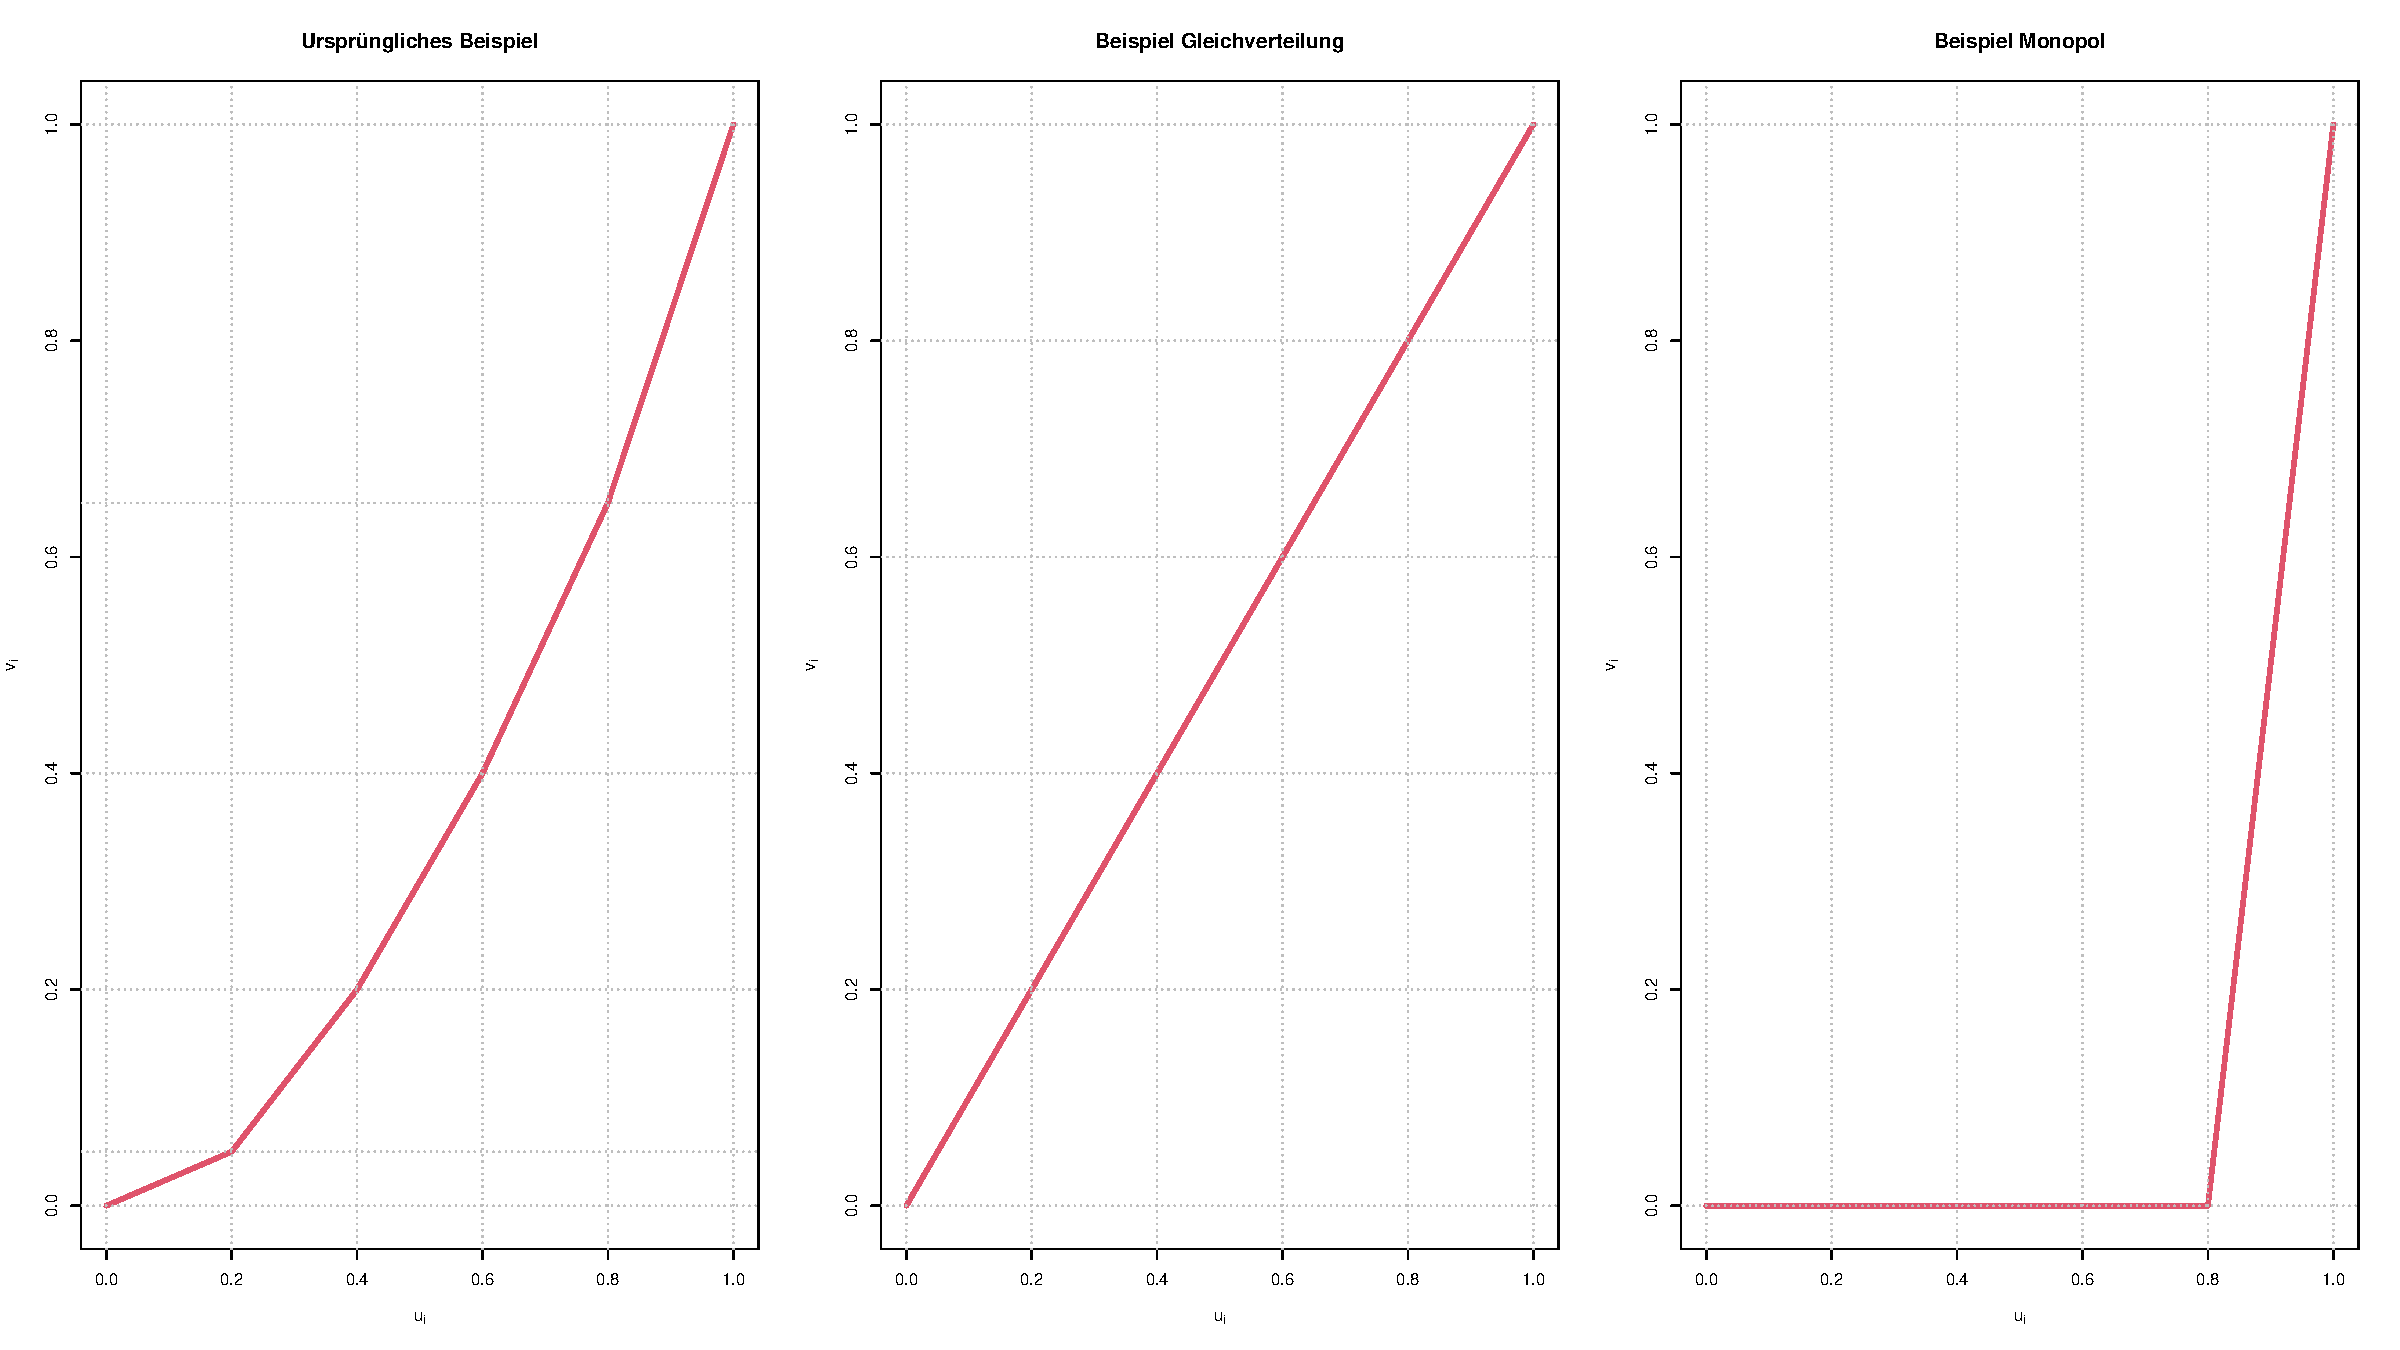
\includegraphics[width = .9\textwidth]{figures/example_lc.pdf}
    \caption{Lorenzkurven zum Beispiel für Individualdaten}
    \label{fig:lk1}
\end{figure}

\noindent Zwischen diesen beiden Extrema gibt es sehr viele Abstufungen von (Un)Gleichverteilung.
Generell lässt sich festhalten: Je weiter der Graph der Lorenzkurve (nach links unten) von der Winkelhalbierende entfernt ist, also je größer die Fläche dazwischen ist, desto ungleicher verteilt, also desto konzentrierter ist ein Merkmal. Vice versa, je näher an der Winkelhalbierenden, desto gleichmäßiger verteilt, als desto weniger konzentriert ist ein Merkmal. Diese angesprochene Fläche spielt auch beim Gini-Koeffizienten (vgl. Kap. \ref{sec:gini}) eine entscheidende Rolle.\\
Weitere Eigenschaften der Lorenzkurve sind, dass sie \textbf{immer} unterhalb der Winkelhalbierenden und niemals darüber verlaufen muss. Da die Merkmalsausprägungen kumuliert (also aufsummiert) werden, kann der Graph nur monoton steigend sein. Zudem muss die Steigung eines Kurvensegments immer größer oder gleich dem vorigen Segments sein, da die Merkmalsausprägungen bei der Lorenzkurve nach Größe geordnet wurden.

\paragraph{Berechnung Lorenzkurve bei gruppierten Daten}
Hat man obige Erklärungen für Individuldaten verstanden, so wird auch das Verständnis für das Vorgehen bei gruppierten Daten nicht schwer fallen. Der erste wichtige, und visuell auffälligste, Unterschied besteht darin, dass die Abstände auf der x-Achse nicht mehr identisch ist. Ansonsten sind die Berechnungen weitestgehend ähnlich zum dem Fall für Individualdaten.\\
Nehmen wir an wir hätten im obigen Beispiel nun nicht mehr 5 Beobachtungen sondern 100. Dabei haben 10 Beobachtungen eine Merkmalsausprägung von 1, 40 haben eine Merkmalsausprägung von 5, 20 eine Merkmalsausprägung von 7 und 30 eine Merkmalsausprägung von 15. Insgesamt entspricht dies einer Merkmalssumme von 800. Die Gruppe mit der geringsten Merkmalsausprägung hätte damit einen Anteil von $\frac{10}{100} = 10\%$ an den Merkmalsträgern und einen Anteil von $\frac{10 \cdot 1}{800} = 0,0125$ an der Merkmalssumme, die beiden Gruppen mit den geringsten  Merkmalsausprägungen einen Anteil von $\frac{10 + 40}{100} = 50\%$ an den Merkmalsträgern und einen Anteil von $\frac{10 \cdot 1 + 40 \cdot 5}{800} = 0,2625$ an der Merkmalssumme, usw.\\Dies führt zu folgenden Punkten für die Lorenzkurve:
$$(0|0);\qquad(0,1|0,0125);\qquad (0,5|0,2625);\qquad (0,7|0,4375);\qquad (1|1)$$

\noindent Abbildung \ref{fig:lk2} zeigt die Lorenzkurve für dieses Beispielszenario.
\begin{figure}[htbp]
    \centering
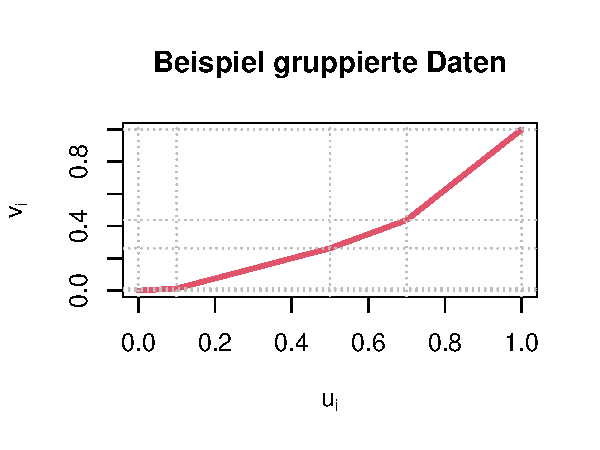
\includegraphics[width = .7\textwidth]{figures/example_lc2.pdf}
    \caption{Lorenzkurve zum Beispiel für gruppierte Daten}
    \label{fig:lk2}
\end{figure}

\noindent \dangersign \textit{Notation:} Um Formeln für gruppierte von Formeln für Individualdaten abzuheben wird eine Tilde verwendet, d.h. x-Werte als $\tilde u_i$ und y-Werte als $\tilde v_i$ bezeichnet.\\
\noindent \dangersign \textit{Anmerkung I:} Die gleiche Lorenzkurve wie in Abbildung \ref{fig:lk2} hätte man auch für die Individualdaten zeichnen können, jedoch wäre dies ein um einiges höherer Aufwand gewesen. In diesem Fall wäre es jedoch möglich gewesen, da wir tatsächlich für jedes Individuum dessen genaue Merkmalsausprägung kennen.\\
\noindent \dangersign \textit{Anmerkung II:} Kennen wir \textbf{nicht} für jedes Individuum dessen genaue Merkmalsausprägung, sondern lediglich einen Gruppenmittelwert, so wird jedem Inidividuum in einer Gruppe diese Gruppenmittelwert als Merkmalsausprägung zugeordnet. Dadurch kann man ganz normal, wie oben für gruppierte Daten gezeigt, vorgehen. Wichtig ist dabei jedoch im Hinterkopf zu behalten, dass damit implizit die Annahme einhergeht, dass innerhalb der Gruppen Gleichverteilung herrscht, da wir jedem Individuum einer Gruppe denselben Wert zuordnen. Diese Annahme muss nicht immer realistisch sein und sollte stets kritisch hinterfragt werden.\\

\noindent \framebox[\textwidth]{\texttt{R-Befehl für die Lorenzkurve: > Lc(data)} \hfill \href{https://www.rdocumentation.org/packages/ineq/versions/0.2-13/topics/Lc}{Dokumentation}}

\noindent \dangersign Die R-Funktion ist \textbf{nicht} Teil von \texttt{base-R} sondern Teil des Paketes \texttt{ineq}. Um diese Funktion verwenden zu können, muss das Paket zunächst installiert werden (\texttt{install.packages("ineq")}) und anschließend importiert werden (\texttt{library(ineq)}).

\clearpage

\subsubsection{Gini-Koeffizient}\label{sec:gini}
Die im vorigen Kapitel erwähnte Fläche $F$, die zwischen dem Graph und der Winkelhalbierenden liegt, stellt die Basis für den Gini-Koeffizienten dar, welcher ein Maß für die relative Konzentration ist. Der Gini ist definiert als "\textit{Zweimal die Fläche zwischen Winkelhalbierender und Lorenzkurve.}"\\

\noindent Kennt man bereits die kumulierten Anteile an der Merkmalssumme (y-Werte der Punkte auf der Lorenzkurve), so ist der Gini recht einfach zu berechnen:
\begin{itemize}
    \item Znächst addiert man jeweils zu jedem Anteilswert den Anteilswert der vorherigen Punktes (angefangen bei 0 bis zur 1): $(v_{i-1}+v_i)$
    \item Diese Summen werden anschließend addiert: $\sum_{i=1}^n (v_{i-1}+v_i)$
    \item und mit $\frac{1}{n}$ multipliziert: $\frac{1}{n}\sum_{i=1}^n (v_{i-1}+v_i)$
    \item Dieses Produkt wird zum Schluss von 1 abgezogen.
\end{itemize}
\begin{align*}
    G=1-\frac{1}{n}\sum_{i=1}^n (v_{i-1} + v_i)
\end{align*}
Für gruppierte Daten ändern sich Vorgehen und Formel nicht dramatisch. Der einzige Unterschied zur obigen Formel besteht darin, dass man mit den Gruppengrößen $n_j$ gewichten muss:

\begin{align*}
    G=1-\frac{1}{n}\sum_{i=1}^n n_j \cdot (\tilde v_{i-1} + \tilde v_i)
\end{align*}

\noindent Man kann sich das ein bisschen wie bei gewichteten arithmetischen Mittel in Kapitel \ref{sec:arithm} vorstellen, da auch dort Unterschiedlichen Gruppengrößen auf ähnliche Art \& Weise Rechnung getragen wird.\\

\noindent Der Wertebereich des Gini-Koeffizient beginnt bei 0, was für eine absolute Gleichverteilung spricht. Dies macht intuitiv Sinn, da bei der absoluten Gleichverteilung die Fläche zwischen Winkelhalbierender und Lorenzkurve nicht existiert. Dass die obere Grenze nicht bei Eins, sondern bei ($\frac{n-1}{n}$, ist auf den ersten Blick vielleicht etwas weniger intuitiv. Bei einem Blick auf das Monopol-Szenario in Abbildung \ref{fig:lk1} sollte jedoch klar werden, dass die Fläche zwischen Winkelhalbierender und Lorenzkurve nicht den Wert 0,5 erreichen kann \& somit der Gini (also das Doppelte dieser Fläche) nicht 1 werden kann. Grund dafür ist das Dreieck, welches unten rechts stets per Konstruktion ausgespart wird. Die Größe dieses ausgesparten Dreieckes hängt von der Anzahl der Merkmalsträger $n$ ab und damit auch der Wertebereich.\\

\noindent Da mit einem variierendem Wertebereich (je nach Anzahl der Merkmalsträger) schwierig Konzentrationen für verschiedene Merkmale verglichen werden können, berechnet man den \textbf{normierten Gini-Koeffizienten $G^+$}.\\
Der normierte Gini-Koeffizient erhält man, indem man den berechneten Gini-Koeffizient mit $\frac{n}{n-1}$ multipliziert:
\begin{align*}
    G^+=\frac{n}{n-1}G
\end{align*}
Der Wertebereich von $G^+$ geht dann noch von 0 bis 1 und ist unabhängig von $n$. Die Konzentration 0 steht dabei für absolute Gleichverteilung, also dafür, dass es \textit{keine} Konzentration gibt, während 1 für eine \textit{vollständige} Konzentration, also für ein Monopol, steht. Somit ist es nun kein Problem mehr verschiedene Merkmale mit unterschiedlichem $n$ in Bezug auf ihre Konzentration zu vergleichen.\\

\noindent \dangersign Bei der Normierung des Gini für gruppierte Daten entspricht $n$ weiterhin der Anzahl der Beobachtungen und \textbf{nicht} der Anzahl der Gruppen.\\

\noindent \textbf{Einschub: Aussagen über Veränderungen}\\
Beim Gini kann man relativ einfach pauschale Aussagen über Veränderungen treffen, solange die Anzahl der Merkmalträger gleich bleibt.
\begin{itemize}
    \item \textit{Beispiel 1: Alle Merkmalsträger erfahren dieselbe relative Steigerung}\\
    Alle Merkmalsträger steigern ihre Merkmalssumme um 10\%. In diesem Fall würde sich Gini nicht verändern, da sich an den Relationen nichts gändert hat.
    \item \textit{Beispiel 2: Alle Merkmalsträger erfahren dieselbe absolute Steigerung}\\
    Alle Merkmalsträger steigern ihre Merkmalssumme um 10 Einheiten. In diesem Fall würde Gini nicht sinken, da in Relationen zueinander nun alle etwas gleichere Anteile besitzen. Man kann sich das gut an einem Extremfall veranschaulichen: Angenommen jeder Merkmalsträger würde seine Merkmalssumme um das 100-fache der bisher größten Ausprägung steigern. Dadurch wurden alle bisher dagewesenen Unterschiede quasi irrelevant werden und jeder hätte nahezu gleich viel. 
\end{itemize}

\noindent \framebox[\textwidth]{\texttt{R-Befehl für den Gini: > Gini(data)} \hfill \href{https://www.rdocumentation.org/packages/ineq/versions/0.2-13/topics/ineq}{Dokumentation}}

\noindent \dangersign Die R-Funktion ist \textbf{nicht} Teil von \texttt{base-R} sondern Teil des Paketes \texttt{ineq}. Um diese Funktion verwenden zu können, muss das Paket zunächst installiert werden (\texttt{install.packages("ineq")}) und anschließend importiert werden (\texttt{library(ineq)}).

\clearpage

\subsection{Aufgaben}

\paragraph{1. Welche Aussagen bzgl. Gini \& Lorenzkurve sind wahr?}

\begin{itemize}
    \item[a)] Die absolute Merkmalssumme ist unerheblich für den Gini. \hfill $\square$
    \item[b)] Höherer Gini bedeutet (global) steilere Lorenzkurve. \hfill $\square$
    \item[c)] Der Gini ist uneingeschränkt geeignet um die Konzentration in zwei Gruppen\\zu vergleichen. \hfill $\square$
    \item[d)] Erhalten alle Merkmalsträger dieselbe prozentuale Steigerung ihres (absoluten)\\Teils der Merkmalssumme, so verändert sich der Gini nicht. \hfill $\square$
\end{itemize}

\paragraph{2. Welche Aussagen bzgl. des Herfindahl-Index sind wahr?}

\begin{itemize}
    \item[a)] Der Herfindahl-Index ist uneingeschränkt geeignet um die Konzentration in zwei\\Gruppen zu vergleichen. \hfill $\square$
    \item[b)] Falls sich die Merkmalssumme ändert, können definitive Aussagen über der Änderung\\des Herfindahl-Index getroffen werden. \hfill $\square$
    \item[c)] Falls sich die Verteilung Merkmalssumme ändert, können definitive Aussagen über der\\Änderung des Herfindahl-Index getroffen werden. \hfill $\square$
    \item[d)] Höherer Herfindahl-Index bedeutet ungleichere Verteilung. \hfill $\square$
\end{itemize}

\paragraph{3. Der Gini für gruppierte Daten ist nur identisch zum "normalen" Gini, falls ..}

\begin{itemize}
    \item[a)] .. alle Gruppen gleich groß sind. \hfill $\square$
    \item[b)] .. absolute Gleichverteilung herrscht. \hfill $\square$
    \item[c)] .. Gleichverteilung innerhalb der Gruppen herrscht. \hfill $\square$
    \item[d)] .. die Anzahl der Gruppen kleiner als 10 ist. \hfill $\square$
\end{itemize}


\clearpage

%%%%%%%%%%%%%%%%%%%%%%%%%%%%%%%%%%%%%
%%%%%%%%%%  KAPITEL 6
%%%%%%%%%%%%%%%%%%%%%%%%%%%%%%%%%%%%%

\section{Zusammenhangsmaße}\label{chap:zshg}
Bis jetzt haben wir stets lediglich eine Variable (bzw. Merkmal) $X$ und dessen Ausprägungen $x_1, x_2,.., x_i$ betrachtet. Auf diese Art und Weise war es uns möglich, Aussagen über dessen Lage, Streuung und Konzentration zu treffen.\\
Da in diesem Kapitel Aussagen über Zusammenhänge getroffen werden sollen bzw. Zusammenhänge quantifiziert werden sollen, werden nun stets \textbf{zwei} Variablen/Merkmale $X$ \& $Y$ gleichzeitig betrachtet. Dies führt dazu, dass die beobachteten Ausprägungen der Merkmale nun folgendermaßen vorliegen: $(x_1; y_1), (x_2; y_2), .., (x_n; y_n)$

\noindent \paragraph{Beispiel:} Wir betrachten nun bei Personen gleichzeitig ihre Körper- ($X$) und ihre Schuhgröße ($Y$). Dies könnte bspw. zu folgender Stichprobe führen: $(185cm;\; 44), (170cm;\; 39), .., (195cm;\; 47)$\\

\noindent Von zentraler Bedeutung für die Quantifizierung von Zusammenhängen ist es, sich im Vorhinein darüber klar zu werden, auf welchen Skalenniveaus die beobachteten Merkmale gemessen werden. Dies hat erhebliche Auswirkungen darauf, welche Zusammenhangsmaße berechnet werden können. Als Richtlinie gilt hier stets: Es kann lediglich ein Zusammenhangsmaß berechnet werden, welches für die Skala desjenigen Merkmals geeignet ist, welches auf der "niedrigeren" Skala gemessen wird.

\noindent \paragraph{Beispiel:} Betrachten wir bei Personen ihr Geschlecht ($X$) und ihr Einkommen ($Y$), so sind nur Zusammenhangsmaße anwendbar, die für nominale Merkmale geeignet sind, da das Merkmal Geschlecht lediglich nominal skaliert ist. Berechnet man stattdessen Betriebszugehörigkeit ($X$) und Einkommen ($Y$), so sind Zusammenhangsmaße für metrische Merkmale anwendbar.

\subsection{Die Kontingenztafel}\label{sec:kont}
Eines der grundlegendsten Instrumente zur gemeinsamen Darstellung zweier Merkmale ist die Kontingenztafel.
Hierbei wird pro unterschiedliche Merkmalsausprägung von $X$ eine Zeile, für jede untersch. Merkmalsausprägung von $Y$ eine Spalte belegt. Dies führt bei der Betrachtung der Merkmale $X$: "Parteizugehörigkeit im Bundestag" (Ausprägungen: \textit{Union, SPD, Grüne, FDP, Linke, AfD}) und $Y$: Geschlecht (Ausprägungen: \textit{weiblich, männlich, divers}) zu einer Kontingenztafel mit 6 Zeilen und 3 Spalten, d.h. einer $(6\times3)$-Kontingenztafel.\\
Die Entscheidung, welche Variable in den Zeilen und welche Variable in den Spalten abgetragen wird, kann mehr oder minder frei getroffen werden. Oftmals wird die Auswahl jedoch nach zwei Kriterien getroffen:
\begin{itemize}
    \item Kann ein betrachtetes Merkmal als "Schichtungsmerkmal" betrachtet werden, so steht es für gewöhnlich in den Zeilen. Ein Schichtungsmerkmal ist eine Variable, die die Stichprobe in verschiedene Gruppen einteilt, wie z.B. "Geschlecht", "Bildungsabschluss" oder "Raucher/Nicht-Raucher".
    \item Vermutet man in den Daten eine kausale Wirkungsstruktur (d.h. ein Merkmal hat einen Einfluss auf das Andere), so steht meist dasjenige Merkmal in den Zeilen, welches als Ursache angesehen wird, z.B.
    bei der Betrachtung von "Raucher/Nicht-Raucher" und "Auftreten von Lungenkrebs ja/nein" würde man das Merkmal "Raucher/Nicht-Raucher" in den Zeilen abtragen.
\end{itemize}
Da in der Kontingenztafel für jede mögliche Ausprägung eines Merkmals eine zusätzliche Zeile bzw. Spalte in der Darstellung benötigt wird, ist sie lediglich für Merkmale mit nicht allzu vielen verschiedenen Ausprägungen sinnvoll. Für metrische Merkmale bedeutet dies, dass diese nur sinnvoll in Kontingenztafeln dargestellt werden können, falls sie vorher in Klassen eingeteilt wurden (bspw. Altersgruppen oder Einkommensklassen).\\
Die inneren Zellen der Kontingenztafeln werden in der Regel mit den absoluten Häufigkeiten $n_{ij}$ ("Wie oft beobachte ich die Ausprägung in der i-ten Zeile von Merkmal $X$ gemeinsam mit der Ausprägung in der j-ten Spalte vom Merkmal $Y$?") oder den relativen Häufigkeiten $f_{ij} = \frac{n_{ij}}{n}$ befüllt.\\
Die (absoluten) Randhäufigkeiten werden mit $n_{i\bullet}$ ("Wie oft beobachte ich die Ausprägung in der i-ten Zeile von Merkmal $X$?") und $n_{\bullet j}$ ("Wie oft beobachte ich die Ausprägung in der j-ten Spalte von Merkmal $Y$?") bezeichnet.\\
Teilt man alle Häufigkeiten der inneren Zellen in der i-ten Zeile durch die Randhäufigkeit der i-ten Zeile, so erhält man die bedingten relativen Häufigkeiten $f_{j|i} = \frac{n_{ij}}{n_{i\bullet}}$. Analog lassen sich auch die bedingen relativen Häufigkeiten $f_{i|j} = \frac{n_{ij}}{n_{\bullet j}}$ für die j-te Spalte bestimmen.

\noindent \paragraph{Beispiel:} \textit{Lungenkrebs bei weiblichen Rauchern}\footnote{Quelle: \tiny{\url{https://www.aerzteblatt.de/archiv/8369/Lungenkrebsrisiko-hoeher-als-bisher-angenommen-Europaweite-Studie-vorgestellt}}}\\

\begin{table}[htbp]
\begin{tabular}{c|cc|c}
    $X$/$Y$         & Lungenkrebs & kein Lungenkrebs & $\sum$ \\
     \hline
    Nicht-Raucher   & 458         & 1598             & 2056 \\
    Raucher         & 877         & 412              & 1289 \\
    \hline
    $\sum$          & 1335        & 2010             & 3345
\end{tabular}
    \caption{\textit{Absolute Häufigkeiten (Lungenkrebsinzidenz bei weiblichen Rauchern)}}
    \label{tab:abs}
\end{table}

\begin{table}[htbp]
\begin{tabular}{c|cc|c}
    $X$/$Y$         & Lungenkrebs & kein Lungenkrebs & $\sum$ \\
     \hline
    Nicht-Raucher   & $\frac{458}{3345}$         & $\frac{1598}{3345}$             & $\frac{2056}{3345}$ \\
    Raucher         & $\frac{877}{3345}$         & $\frac{412}{3345}$              & $\frac{1289}{3345}$ \\
    \hline
    $\sum$          & $\frac{1335}{3345}$        & $\frac{2010}{3345}$             & 1
\end{tabular}
    \caption{\textit{Relative Häufigkeiten (Lungenkrebsinzidenz bei weiblichen Rauchern)}}
    \label{tab:rel}
\end{table}

\noindent \framebox[\textwidth]{\texttt{R-Befehl für Kontingenztafeln: > table(data\$x, data\$y)} \hfill \href{https://www.rdocumentation.org/packages/base/versions/3.6.2/topics/table}{Dokumentation}}

\clearpage

\begin{table}[htbp]
\begin{tabular}{c|cc|c}
    $X$/$Y$         & Lungenkrebs & kein Lungenkrebs & $\sum$ \\
     \hline
    Nicht-Raucher   & $\frac{458}{2056}$         & $\frac{1598}{2056}$             & 1 \\
    Raucher         & $\frac{877}{1289}$         & $\frac{412}{1289}$              & 1 \\
    \hline
\end{tabular}
    \caption{\textit{Bedingt auf Raucher/Nicht-Raucher (Lungenkrebsinzidenz bei weiblichen Rauchern)}}
    \label{tab:bed1}
\end{table}

\begin{table}[htbp!]
\begin{tabular}{c|cc|}
    $X$/$Y$         & Lungenkrebs & kein Lungenkrebs \\
     \hline
    Nicht-Raucher   & $\frac{458}{1335}$         & $\frac{1598}{2010}$   \\      
    Raucher         & $\frac{877}{1335}$         & $\frac{412}{2010}$    \\      
    \hline
    $\sum$          & 1         & 1           
\end{tabular}
    \caption{\textit{Bedingt auf Lungenkrebs-Status (Lungenkrebsinzidenz bei weiblichen Rauchern)}}
    \label{tab:bed2}
\end{table}

\noindent \framebox[\textwidth]{\texttt{R-Befehl für (bedingte) Kontingenztafeln: > prop.table(data)} \hfill \href{https://www.rdocumentation.org/packages/base/versions/3.6.2/topics/prop.table}{Dokumentation}}

\subsection{Unabhängigkeit}\label{sec:unabh}
Ein zentrales Konzept bei der Betrachtung von Zusammenhängen ist die \textit{Unabhängigkeit}.\\
Betrachtet man in Tabelle \ref{tab:abs} die Randhäufigkeiten $n_{\bullet j}$ der Spalten, so erkennt man das Verhältnis von Lungenkrebs zu Nicht-Lungenkrebs, unabhängig davon ob jemand geraucht hat oder nicht. Dieses Verhältnis liegt bei etwas mehr als 2 zu 3. Betrachtet man nun lediglich die Häufigkeiten in der ersten Zeile (d.h. nur die Nicht-Raucher) $n_{11}$ und $n_{12}$, so erkennt man, dass unter diesen Beobachtungen das Verhältnis von Lungenkrebs zu Nicht-Lungenkrebs bei ca. 1 zu 4 liegt (bei den Nicht-Lungenkrebs-Fällen liegt es bei etwas mehr als 2 zu 1). Somit scheint es einen Zusammenhang zwischen Rauchen und dem Auftreten von Lungenkrebs zu geben, da man unter Unabhängigkeit erwarten würde, in beiden Gruppen (Nicht-Raucher und Raucher) dasselbe Verhältnis, nämlich das der Randhäufigkeiten zu beobachten. Berechenbar sind die \textit{unter Unabhängigkeit erwarteten absoluten Häufigkeiten} über die Formel $\hat{n_{ij}} = \frac{n_{i\bullet} \cdot n_{\bullet j}}{n}$.

\noindent \paragraph{Fortsetzung Beispiel:} \textit{Lungenkrebs bei weiblichen Rauchern}
\begin{table}[htbp]
\begin{tabular}{c|cc|c}
    $X$/$Y$         & Lungenkrebs & kein Lungenkrebs & $\sum$ \\
     \hline
    Nicht-Raucher   & $\frac{2056\cdot1335}{3345} = 820,5561$         & $\frac{2056\cdot2010}{3345} = 1235,4439$             & 2056 \\
    Raucher         & $\frac{1289\cdot1335}{3345} = 514,4439$         & $\frac{1289\cdot2010}{3345} = 774,5561$             & 1289 \\
    \hline
    $\sum$          & 1335        & 2010             & 3345
\end{tabular}
    \caption{\textit{Unter Unabhängigkeit erwartete absolute Häufigkeiten}}
    \label{tab:abs-unabh}
\end{table}

\noindent Betrachtet man in dieser Häufigkeitstabelle nun die Verhältnisse von Lungenkrebs zu Nicht-Lungen\-krebs bei den Rauchern bzw. bei den Nicht-Rauchern, so erkennt man, dass das Verhältnis in beiden Gruppen jeweils bei ca. 2 zu 3 liegt und somit dem Verhältnis der Randhäufigkeiten der Spalten entspricht.

\clearpage

\subsection{Zusammenhangsmaße für nominale Merkmale}\label{sec:zshg-nom}
Dadurch, dass einfach berechenbar ist, wie eine Häufigkeitstabelle unter Unabhängigkeit der beiden Merkmale aussieht (vgl. Tabelle \ref{tab:abs-unabh}), kann man nun messen wie stark die tatsächlich beobachtete Häufigkeitstabelle davon abweicht. Um diese beobachteten Abweichungen in eine einzige Maßzahl zusammenzufassen, geht man wie folgt vor:
\begin{itemize}
    \item Man bildet für jede Zelle die Differenz aus beobachteter absoluter Häufigkeit und unter Unabhängigkeit erwarteter absoluter Häufigkeit: $n_{ij} - \hat{n_{ij}}$ 
    \item Man quadriert diese Differenzen, damit sich negative und positive Abweichungen später beim Aufsummieren nicht gegenseitig aufheben: $(n_{ij} - \hat{n_{ij}})^2$ 
    \item Man teilt diese quadrierten Differenzen durch die $\hat{n_{ij}}$, d.h. man setzt sie ins Verhältnis zu dem Wert, den man eigentlich erwartet hätte: $\frac{(n_{ij} - \hat{n_{ij}})^2}{\hat{n_{ij}}}$
    \item Man summiert diese Werte der einzelnen Zellen auf: $\sum_{i=1}^k\sum_{j=1}^l \frac{(n_{ij} - \hat{n_{ij}})^2}{\hat{n_{ij}}}$
\end{itemize}
Die Maßzahl, welche durch diese Vorgehensweise berechnet wird, nennt sich $\chi^2$-Koeffizient und nimmt bei Unabhängigkeit (d.h. unter Unabhängigkeit erwartete sind gleich den beobachteten absoluten Häufigkeiten) den Wert 0 an, bei Abhängigkeit hingegen sehr hohe Werte. Diese Maßzahl besitzt jedoch noch einige gravierende Nachteile:
\begin{itemize}
    \item Je mehr Beobachtungen wir in unserer Stichprobe haben, desto leichter sind hohe Abweichungen zu beobachten, d.h. desto größer wird \textit{tendenziell} $\chi^2$
    \item Je mehr Zellen die Kontingenztafel besitzt, desto mehr Abweichungen sind zu beobachten, d.h. desto größer wird \textit{tendenziell} $\chi^2$
\end{itemize}
Um diesen Nachteilen entgegenzutreten existieren verschiedene Erweiterungen, welche eine (oder beide) dieser Einschränkungen beheben.\\

\noindent \framebox[\textwidth]{\texttt{R-Befehl für $\chi^2$: > chisq.test(data\$x, data\$y)} \hfill \href{https://www.rdocumentation.org/packages/stats/versions/3.6.2/topics/chisq.test}{Dokumentation}}

\noindent \dangersign Diese R-Funktion führt neben der Berechnung von $\chi^2$ auch den zugehörigen $\chi^2$-Unabhängigkeits\-test durch. Dies ist erst Teil des Stoffs von Statistik II (vgl. Kap. \ref{sec:chitest2}) und kann vorläufig ignoriert werden. Der Wert \texttt{X-squared} in der Ausgabe entspricht dem $\chi^2$-Koeffizienten.

\paragraph{Loslösung vom Stichprobenumfang}
Der $\Phi$-Koeffizient und der Kontingenzkoeffizient $C$ sind zwei Möglichkeiten um den Wertebereich von $\chi^2$ vom Stichprobenumfang zu lösen. Sie berechnen sich auf folgende, leicht unterschiedliche Weisen
\begin{align*}
    \Phi &= \sqrt{\frac{\chi^2}{n}}, \qquad 0 \leq \Phi \leq \sqrt{min(k,l)-1}\\
    C &= \sqrt{\frac{\chi^2}{\chi^2 + n}}, \qquad 0 \leq C \leq \sqrt{\frac{min(k,l)-1}{min(k,l)}}
\end{align*}

\noindent \dangersign \textbf{Wichtig:} Die Zeilen- und Spaltenzahl werden in diesem Kontext mit $k$ \& $l$ bezeichnet.\\

\noindent Eine Berechnung diese beiden Maßzahlen macht Sinn, wenn wir die Zusammenhänge aus zwei Kontingenztafeln vergleichen wollen, bei denen zwar der Stichprobenumfang, nicht aber jedoch die Dimensionen der Kontingenztafel unterschiedlich sind. Beispielsweise könnte man den berechneten Zusammenhang aus Tabelle \ref{tab:abs} mit einer Gruppe von männlichen Rauchern vergleichen. Hier wären dann die Dimensionen der beiden Tafeln identisch, die Stichprobenumfänge könnten sich jedoch unterscheiden.\\

\noindent \framebox[\textwidth]{\texttt{R-Befehl für den $\Phi$-Koeffizient: > Phi(data\$x, data\$y)} \hfill \href{https://www.rdocumentation.org/packages/DescTools/versions/0.99.37/topics/Association\%20measures}{Dokumentation}}\\
\noindent \framebox[\textwidth]{\texttt{R-Befehl für den $C$: > ContCoef(data\$x, data\$y)}\\ \mbox{} \hfill \href{https://www.rdocumentation.org/packages/DescTools/versions/0.99.37/topics/Association\%20measures}{Dokumentation}}

\noindent \dangersign Die R-Funktionen sind \textbf{nicht} Teil von \texttt{base-R} sondern Teil des Paketes \texttt{DescTools}. Dieses muss zunächst installiert (\texttt{install.packages("DescTools")}) und anschließend importiert werden (\texttt{library(DescTools)}).

\paragraph{Loslösung von der Dimension der Kontingenztafel}
Möchte man diese beiden Maße nun auch noch von der Dimension der Kontingenztafel loslösen, so kann man dies durch Berechnung von $Cramers\; V$ oder des korrigierten Kontingenzkoeffizienten $C_{korr}$ tun:
\begin{align*}
    V &= \sqrt{\frac{\chi^2}{n\cdot(min(k,l)-1)}}, \qquad 0 \leq V \leq 1\\
    C_{korr} &= \sqrt{\frac{min(k,l)}{min(k,l)-1}}\cdot\underbrace{\sqrt{\frac{\chi^2}{\chi^2 + n}}}_{C}, \qquad 0 \leq C_{korr} \leq 1
\end{align*}

\noindent Eine Berechnung diese beiden Maßzahlen macht Sinn, wenn wir die Zusammenhänge aus zwei Kontingenztafeln vergleichen wollen, bei denen sowohl der Stichprobenumfang, als auch die Dimensionen der Kontingenztafel unterschiedlich sind. Beispielsweise könnte man den berechneten Zusammenhang aus Tabelle \ref{tab:abs} mit einer Gruppe von männlichen Rauchern vergleichen, bei denen nicht nur die Lungenkrebsinzidenz sondern auch das Auftreten anderer Krebsarten betrachtet wird. Hier wären dann auch die Dimensionen der beiden Tafeln unterschiedliche, da die Kontingenztafel der Männer mehr Spalten besäße als die der Frauen.\\

\noindent  \framebox[\textwidth]{\texttt{R-Befehl für den Cramers V: > CramerV(data\$x, data\$y)} \hfill \href{https://www.rdocumentation.org/packages/DescTools/versions/0.99.37/topics/Association\%20measures}{Dokumentation}}\\
\noindent  \framebox[\textwidth]{\texttt{R-Befehl für $C_{korr}$: > ContCoef(.., correct = TRUE)} \hfill \href{https://www.rdocumentation.org/packages/DescTools/versions/0.99.37/topics/Association\%20measures}{Dokumentation}}

\noindent \dangersign Die R-Funktionen sind \textbf{nicht} Teil von \texttt{base-R} sondern Teil des Paketes \texttt{DescTools}. Dieses muss zunächst installiert (\texttt{install.packages("DescTools")}) und anschließend importiert werden (\texttt{library(DescTools)}).

\clearpage

\subsection{Odds Ratio}
Der Odds-Ratio ist ein Maß, welche speziell für Vier-Felder-Tafeln definiert ist. Durch Zwischenschritte über das (relative) Risiko bis letztendlich hin zum Odds Ratio lässt er sich gut nachvoll\-ziehbar erklären.

\begin{table}[htbp]
\centering
\begin{tabular}{c|cc|c}
&$y_1$&$y_2$&$\sum$\\
\hline
$x_1$ & a&b&a+b\\
$x_2$&c&d&c+d\\
\hline
$\sum$&a+c&b+d&n
\end{tabular}
    \caption{\textit{Allgemeine Darstellung einer $2\times2$-Kontingenztafel (Vier-Felder-Tafel)}}
    \label{tab:2k2}
\end{table}

\paragraph{Risiko} Betracht man zunächst ein \textit{Risikomerkmal}, so kann man für dieses Risikomerkmal die Wahrscheinlichkeit bestimmen, dass es eintritt. Diese Wahrscheinlichkeit wird als Risiko bezeichnet. So könnte man bspw. für Tabelle \ref{tab:abs} das Risiko bestimmen, dass eine Frau an Lungenkrebs erkrankt: Entweder für die gesamte Population ($\frac{1335}{3345}$) oder für eine bestimmte "Schicht" (z.B. für die Raucher: $\frac{877}{1289}$). Im Folgenden werden wir vom Geschlecht als \textit{Schichtungsmerkmal} und vom Lungenkrebs als \textit{Risikomerkmal} sprechen.

\paragraph{Relatives Risiko} Möchte man nun die Risiken in zwei verschiedenen Schichten miteinander vergleichen, so bietet sich das relative Risiko als Maßzahl an. Hierbei dividiert man die Risiken zweier Schichten durcheinander, z.B. das Risiko für Lungenkrebs bei den Rauchern und das Risiko für Lungenkrebs bei den Nicht-Rauchern:
\begin{align*}
    RR_{Lungenkrebs} = \dfrac{\frac{877}{1289}}{\frac{458}{2056}} = \dfrac{0,68}{0,22} = 3,09
\end{align*}
Dieser Wert bedeutet, dass das Risiko für Lungenkrebs bei den Rauchern ca. dreimal so hoch ist wie bei den Nicht-Rauchern. Welches Schichtungsmerkmal dabei im Zähler steht ist nicht fix vorgegeben, ist jedoch für die Interpretation des Ergebnisses im Nachhinein wichtig. Man könnte also auch die Nicht-Raucher in den Zähler packen: 
\begin{align*}
    RR_{Lungenkrebs} = \dfrac{\frac{458}{2056}}{\frac{877}{1289}} = \dfrac{0,22}{0,68} = 0,32
\end{align*}
Die Interpretation wäre hier, dass das Risiko für Lungenkrebs bei den Nicht-Rauchern lediglich einem Drittel des Risikos bei den Rauchern entspricht. Letztlich die gleiche Aussage wie zuvor, nur auf andere Art und Weise ausgedrückt.

\paragraph{Chance} Vergleicht man die Risiken von zwei konkurrierenden Risikomerkmalen für ein Schichtungsmerkmal, so spricht man von der Chance oder auf Englisch \textit{Odds}. Man spricht dabei immer von der Chance auf dasjenige Merkmal, dessen Risiko im Zähler steht, d.h. $$\frac{\mbox{Risiko für "Lungenkrebs" bei Rauchern}}{\mbox{Risiko für "kein Lungenkrebs" bei Rauchern}} = \dfrac{\frac{877}{1289}}{\frac{412}{1289}} = \dfrac{877}{412} = 2,13$$
beschreibt die Chance für Lungenkrebs (bei Rauchern), während
$$\frac{\mbox{Risiko für "kein Lungenkrebs" bei Rauchern}}{\mbox{Risiko für "Lungenkrebs" bei Rauchern}} = \dfrac{\frac{412}{1289}}{\frac{877}{1289}} = \dfrac{877}{412} = 0,47$$
die Chance für kein Lungenkrebs (bei Rauchern) beschreibt. Letztendliche liefern beide Berechnungen jedoch wieder dieselbe Aussage.

\paragraph{Odds Ratio} Ähnlich wie beim relativen Risiko möchte man auch beim Odds Ratio zwei verschiedene Schichten miteinander vergleichen, aber nicht hinsichtlich der Risiken sondern hinsichtlich der Chancen. Hierbei dividiert man also die Chancen zweier Schichten durcheinander, z.B. die Chance für Lungenkrebs bei den Nicht-Rauchern und die Chance für Lungenkrebs bei den Rauchern:
\begin{align*}
    OR = \dfrac{\frac{458}{1598}}{\frac{877}{412}} = 0,02
\end{align*}
Dieser Wert bedeutet, dass die Chance für Lungenkrebs bei den Nicht-Rauchern ca. 0,02 mal so hoch ist wie bei den Rauchern. Welches Schichtungsmerkmal dabei im Zähler steht ist nicht fix vorgegeben, ist jedoch für die Interpretation des Ergebnisses im Nachhinein wichtig. Man könnte also auch die Raucher in den Zähler packen: 
\begin{align*}
    OR = \dfrac{\frac{877}{412}}{\frac{458}{1598}} = 58,65
\end{align*}
Die Interpretation wäre hier, dass die Chance für Lungenkrebs bei den Rauchern 58,65 mal dem der Nicht-Raucher entspricht. Letztlich die gleiche Aussage wie zuvor, nur auf andere Art und Weise ausgedrückt.\\

\noindent \dangersign Bei der generellen Formel für den Odds Ratio steht (sofern nicht explizit etwas anderes gesagt wird) das Schichtungsmerkmal aus der ersten Zeile im Zähler, was man an der Formel (bezogen auf Tabelle \ref{tab:2k2}) erkennen kann:
\begin{align*}
    OR = \dfrac{\frac{a}{b}}{\frac{c}{d}} = \dfrac{a \cdot d}{b \cdot c}
\end{align*}\\

\noindent  \framebox[\textwidth]{\texttt{R-Befehl für den Odds Ratio: > OddsRatio(data)} \hfill \href{https://www.rdocumentation.org/packages/DescTools/versions/0.99.37/topics/OddsRatio}{Dokumentation}}

\noindent \dangersign Die R-Funktion ist \textbf{nicht} Teil von \texttt{base-R} sondern Teil des Paketes \texttt{DescTools}. Dieses muss zunächst installiert (\texttt{install.packages("DescTools")}) und anschließend importiert werden (\texttt{library(DescTools)}).

\clearpage

\subsection{Zusammenhangsmaße für ordinale Merkmale}\label{sec:zshg-ord}
Bei ordinalen Daten haben wir, durch die Möglichkeit die Daten zu ordnen, mehr Informationsgehalt. Deshalb macht es hier Sinn, andere Zusammenhangsmaße zu benutzen, damit dieser Informationsgehalt nicht verloren geht. Die Idee hinter den ordinalen Zusammenhangsmaßen ist die, dass man jede Beobachtung mit jeder anderen Beobachtung vergleicht und sich dabei anschaut, wie diese zueinander stehen. Dabei ordnet man solche Beobachtungspaare als \textit{konkordant}, \textit{diskordant} oder als \textit{Bindung} ein.

\paragraph{Konkordanz} liegt vor, wenn sich X und Y in die gleiche Richtung bewegen, also die Beobachtung mit einem größeren x-Wert auch einen größeren y-Wert aufweist.\\
\textit{Beispiel:} $(x_1,y_1)=(2,3)$ ist konkordant zu $(x_2,y_2)=(4,8)$, denn beim Übergang von der ersten zur zweiten Beobachtung steigt X von 2 auf 4 und Y von 3 auf 8. Konkordanz läge ebenfalls vor, wenn X fallen \& Y ebenfalls fallen würde. Somit bewegen sich beide Werte in die gleiche Richtung. "\textit{Je größer X, desto größer Y}" spricht für einen positiven/gleichgerichteten Zusammenhang.

\paragraph{Diskordanz} ist das Gegenteil, d.h. wenn X sich in eine andere Richtung als Y bewegt.\\
\textit{Beispiel} hierfür ist $(x_1,y_1)=(2,3)$ und $(x_2,y_2)=(5,1)$. Beim Übergang von der ersten zur zweiten Beobachtung steigt X von 2 auf 5, Y sinkt jedoch von 3 auf 1. Diskordanz läge ebenfalls vor, wenn X fallen \& Y steigen würde. Es geht somit nur um die Entwicklung in unterschiedliche Richtungen, also um einen negativen Zusammenhang.

\paragraph{Bindungen (Ties)} liegen vor wenn sich ein Wert verändert, der andere jedoch gleich bleibt.\\ 
\textit{Beispiel} für eine Bindung in X wäre hier $(x_1,y_1)=(3,5)$ und $(x_2,y_2)=(3,8)$ bzw. für eine Bindung in Y $(x_1,y_1)=(4,7)$ und $(x_2,y_2)(2,7)$. Bindungen enthalten keine Aussagekraft für mögliche Zusammenhänge.\\

\noindent Um basierend auf einer Kontigenztafel die Anzahlen der konkordanten/diskordanten Paare und der Bindungen zu berechne, ist es zunächst einmal wichtig, dass die Merkmalsausprägungen in den Zeilen \& Spalten geordnet sind. Ist dies nicht der Fall, ist ein strukturiertes Vorgehen unmöglich. Ist dies gewährleistet, gibt es eine bestimmte, strukturierte Vorgehensweise:\\

\noindent \textbf{Konkordante Paare:}
\begin{itemize}
    \item Man beginnt \textbf{links} oben (Zelle für die kleinste Ausprägung sowohl von X, als auch von Y).
    \item Man multipliziert die Beobachtungszahl in dieser Zelle mit allen Beobachtungszahlen, die in Zellen \textit{unter} UND \textit{rechts} von dieser Zelle liegen.\\
    Grund: Diese Beobachtungen haben sowohl größere x-Werte, als auch größere y-Werte.
    \item Man wendet dieses Prinzip auf \textbf{jede} Zelle in der Tabelle an und summiert die Werte für die einzelnen Zellen am Schluss auf, um die Gesamtzahl konkordanter Paare zu erhalten.
\end{itemize}

\noindent \textbf{Diskordante Paare}
\begin{itemize}
    \item Man beginnt \textbf{rechts} oben (Zelle für die kleinste Ausprägung von X und die größte von Y).
    \item Anders als bei der Konkordanz multipliziert man die Beobachtungszahl in dieser Zelle mit allen Beobachtungszahlen, die in Zellen \textit{unter} UND \textit{links} von dieser Zelle liegen.\\
    Grund: Diese Beobachtungen haben sowohl größere x-Werte, jedoch kleinere y-Werte.
    \item Man wendet dieses Prinzip auf \textbf{jede} Zelle in der Tabelle an und summiert die Werte für die einzelnen Zellen am Schluss auf, um die Gesamtzahl diskordanter Paare zu erhalten.
\end{itemize}

\noindent \textbf{Bindungen (Ties) in X}
\begin{itemize}
    \item Man beginnt \textbf{links} oben (Zelle für die kleinste Ausprägung sowohl von X, als auch von Y).
    \item Man multipliziert die Beobachtungszahl in dieser Zelle mit allen Beobachtungszahlen, die in Zellen \textit{in derselben Zeile} wie diese Zelle liegen.\\
    Grund: Diese Beobachtungen haben den gleichen x-Wert, jedoch andere y-Werte.
    \item Man wendet dieses Prinzip auf \textbf{jede} Zelle in der Tabelle an und summiert die Werte für die einzelnen Zellen am Schluss auf, um die Gesamtzahl an Bindungen in X zu erhalten.
\end{itemize}

\noindent \textbf{Bindungen (Ties) in Y}
\begin{itemize}
    \item Man beginnt \textbf{links} oben (Zelle für die kleinste Ausprägung sowohl von X, als auch von Y).
    \item Man multipliziert die Beobachtungszahl in dieser Zelle mit allen Beobachtungszahlen, die in Zellen \textit{in derselben Spalte} wie diese Zelle liegen.\\
    Grund: Diese Beobachtungen haben andere x-Werte, jedoch den gleichen y-Wert.
    \item Man wendet dieses Prinzip auf \textbf{jede} Zelle in der Tabelle an und summiert die Werte für die einzelnen Zellen am Schluss auf, um die Gesamtzahl an Bindungen in Y zu erhalten.
\end{itemize}

\noindent \dangersign \textit{Notation:} Für alle nachfolgend aufgeführten Formeln werden die Anzahlen der konkordanten \& diskordanten Paare, sowie der Bindungen in X bzw. Y, mit $K$, $D$, $T_x$ \& $T_y$ bezeichnet.\\

\noindent Ein schönes Beispiel für die Berechnung von $K$ und $D$ findet sich hier: \hfill \href{https://support.minitab.com/de-de/minitab/19/help-and-how-to/statistics/tables/supporting-topics/other-statistics-and-tests/what-are-concordant-and-discordant-pairs/}{Beispiel}\\

\noindent Mit der Kenntnis über die Anzahlen der konkordanten \& diskordanten Paare, sowie der Bindungen in X bzw. Y, kann man nun einige Zusammenhangsmaße berechnen.

\clearpage

\subsubsection{Gamma nach Goodman and Kruskal}\label{sec:gamma}
Das $\gamma$ nach Goodman and Kruskal quantifiziert den Zusammenhang zwischen zwei Merkmalen allein auf Grundlage der konkordanten und diskordanten Paare. Im Zähler wird die Differenz der beiden Werte berechnet und im Nenner werden die beiden addiert.
\begin{align*}
    \gamma=\frac{K-D}{K+D}
\end{align*}

Aufgrund der Differenzenbildung im Zähler dann der Bruch sowohl positive, als auch negative Werte annehmen. Liegen nur diskordante Paare vor (d.h. $K = 0$), besteht ein perfekter negativer Zusammenhang und $\gamma$ nimmt den Wert -1 an. Liegen ausschließlich konkordante Paare vor (d.h. $D = 0$), so spricht man von einem perfekten positiven Zusammenhang und $\gamma$ beträgt +1.\\
Abstufungen im negativen \& positiven Bereich deuten auf \textit{tendenziell} negative bzw. positive Zusammenhänge hin und je näher der Wert betragsmäßig an der 1 liegt, als desto stärker wird der Zusammenhang bewertet. Liegen (annähernd) gleich viele konkordante und diskorante Paar vor, so ist wird $\gamma$ (annähernd) einen Wert von 0 annehmen und es ist kein eindeutiger Zusammenhang erkennbar.\\

\noindent \dangersign Im Gegensatz zu den den Maßen für nominale Merkmale beinhaltet $\gamma$ nicht nur eine Aussage über die \textbf{Stärke}, sondern auch über die \textbf{Richtung} des Zusammenhangs. Dies spiegelt sich im Wertebereich wieder, der in Kapitel \ref{sec:zshg-nom} bei allen Maßen nur im positiven lag und bei den Maßen in diesem Kapitel sowohl im positiven als auch im negativen liegt.\\

\noindent \dangersign Bei der Berechnung von $\gamma$ werden die Bindungen komplett außen vor gelassen werden. Dies führt (tendenziell) zu einer Überschätzung des Zusammenhangs, da Beobachtungspaare die gegen einen Zusammenhang sprechen (die Bindungen) ignoriert werden. Die $\tau$-Maße beheben dieses Problem.\\

\noindent  \framebox[\textwidth]{\texttt{R-Befehl für $\gamma$: > GoodmanKruskalGamma(data)} \hfill \href{https://www.rdocumentation.org/packages/DescTools/versions/0.99.37/topics/GoodmanKruskalGamma}{Dokumentation}}

\noindent \dangersign Die R-Funktion ist \textbf{nicht} Teil von \texttt{base-R} sondern Teil des Paketes \texttt{DescTools}. Dieses muss zunächst installiert (\texttt{install.packages("DescTools")}) und anschließend importiert werden (\texttt{library(DescTools)}).

\clearpage

\subsubsection{Tau-Maße}\label{sec:tau}

\paragraph{Kendalls $\tau_b$}
Hier werden die $T_x$ und $T_y$ Bindungen berücksichtigt. Der Zähler ist identisch zu $\gamma$, jedoch werden im Nenner die Bindungen mit eingerechnet:
\begin{align*}
    \tau_b = \frac{K-D}{\sqrt{(K+D+T_x)(K+D+T_y)}}
\end{align*}

\noindent \dangersign Liegen keine Bindungen vor, so kollabiert der Nenner zu 
$$\sqrt{(K+D+0)(K+D+0)} = \sqrt{(K+D)^2} = K+D\;,$$ sodass $\tau_b$ identisch zu $\gamma$ ist.\\

\noindent  \framebox[\textwidth]{\texttt{R-Befehl für $\tau_b$: > cor(data\$x, data\$y, method = "kendall")} \hfill \href{https://www.rdocumentation.org/packages/stats/versions/3.6.2/topics/cor}{Dokumentation}}

\paragraph{Kendalls/Stuarts $\tau_c$}
Bei Kendalls/Stuarts $\tau_c$ werden nicht die Bindungen, sondern das Minimum aus der Spaltenzahl und der Zeilenanzahl in der Berechnung berücksichtigt. Ausgangspunkt ist jedoch weiterhin die Differenz aus den Anzahlen der konkordanten und diskordanten Paare im Zähler.
\begin{align*}
    \tau_c = \frac{2min(k,l) (K-D)}{n^2(min(k,l)-1)}
\end{align*}

\noindent \dangersign \textbf{Remember:} Die Zeilen- und Spaltenzahl werden in diesem Kontext mit $k$ \& $l$ bezeichnet.\\

\noindent  \framebox[\textwidth]{\texttt{R-Befehl für $\tau_c$: > StuartTauC(data)} \hfill \href{https://www.rdocumentation.org/packages/DescTools/versions/0.99.37/topics/StuartTauC}{Dokumentation}}

\noindent \dangersign Die R-Funktion ist \textbf{nicht} Teil von \texttt{base-R} sondern Teil des Paketes \texttt{DescTools}. Dieses muss zunächst installiert (\texttt{install.packages("DescTools")}) und anschließend importiert werden (\texttt{library(DescTools)}).

\noindent \dangersign Kendalls $tau_b$ ist das wohl gebräuchlichste diese drei Maße, was man auch daran erkennen kann, dass es in \textit{base-R} verfügbar ist während die anderen beiden nur über eine spezielles Paket verfügbar sind.

\subsubsection{Rangkorrelationskoeffizient nach Spearman}
Der Spearman Korrelations-Koeffizient ($r_{SP}$) wird auch Rangkorrelationskoeffizient genannt, da man nicht die Abstände der echten Datenpunkte zueinandner in Beziehung setzt, sondern nur die \textit{Rangabstände} betrachtet. Dies ist auch der große Unterschied zum Korrelationskoeffizient nach Bravais-Pearson (vgl. Kap. \ref{sec:cor-bp}).

\paragraph{Berechnung:} Die Basis bildet eine Auflistung der Beobachtungen und die Zuordnung der passende Ränge zu den einzelnen Merkmalsausprägungen. Anschließend bildet man \textit{für jeder Beobachtung} die Differenz des Ranges von $x_i$ und des Ranges von $y_i$. Auf Basis dieser Rangdifferenzen $d_i$ wird $r_{SP}$ schließlich berechnet:

\begin{align*}
    r_{SP}=1-\frac{6\sum_{i=1}^nd_i^2}{n(n^2-1)}
\end{align*}

\noindent \dangersign Diese Formel funktioniert nur wenn \textbf{keine} Bindungen vorliegen. Ist dies doch der Fall, so muss man dafür korrigieren (siehe unten).

\paragraph{Korrigierter Rangkorrelationskoeffizient nach Spearman} Liegen \textit{Bindungen} innerhalb eines Merkmals oder beider Merkmale vor, wird die Bestimmung der Ränge etwas komplexer. Zusätzlich zu den $d_i$ kommen hier noch $b_j$ und $c_k$ hinzu.\\

\noindent \dangersign $b_j$ und $c_k$ haben einen anderen Index als die $d_i$. Während $i$ der Laufindex für die Beobachtungen ist, beziehen sich $j$ und $k$ auf die verschiedenen Merkmalsausprägungnen von X bzw. Y.\\

\noindent Die $b_j$ sind die Anzahlen, die angeben wie oft die unterschiedlichen Merkmalsausprägungen beim Merkmal X jeweils auftreten. Die $c_k$ bedeuten analog dazu dasselbe für Y.\\
Liegen keine Bindungen vor, so passieren zwei Dinge: Alle $b_j$ und alle $c_k$ nehmen den Wert 1 an, da jede Merkmalsausprägung nur einmal vorkommt. Die Teile der Formel mit $b_j$ und $c_k$ werden dadurch gleich Null und fallen also weg. Passiert dies, so reduziert sich die Formel auf die obige Formel, welche also nur einen Spezielfall der nachfolgenden Formel darstellt:

\begin{align*}
    r_{SP}=\frac{n(n^2-1)-\frac{1}{2}\sum_jb_j(b_j^2-1)-\frac{1}{2}\sum_kc_k(c_k^2-1)-6\sum_id_i^2}{\sqrt{n(n^2-1)-\sum_jb_j(b_j^2-1)}\sqrt{n(n^2-1)-\sum_kc_k(c_k^2-1)}}
\end{align*}

\noindent Der Wertebereich von $r_{SP}$ geht von -1 bis +1 und auch die Interpretation ist analog zu den $\gamma$- \& $\tau$-Maßen: Bei $r_{SP}<0$ liegt ein negativer Zusammenhang zwischen den beiden Merkmalen vor, bei $r_{SP}>0$ liegt ein positiver Zusammenhang vor und bei $r_{SP}=0$ liegt kein Zusammenhang vor. Zudem ist $r_{SP}$ dimensionslos und symmetrisch. Symmetrisch bedeutet, dass $r_{SP}(X,Y) = r_{SP}(Y,X)$.\\

\noindent \framebox[\textwidth]{\texttt{R-Befehl für $r_{SP}$: > cor(data\$x, data\$y, method = "spearman")} \hfill \href{https://www.rdocumentation.org/packages/stats/versions/3.6.2/topics/cor}{Dokumentation}}\\

\noindent \dangersign Auch wenn alle Maße aus diesem Kapitel für ordinale Merkmale gedacht sind, kann man sie auch für metrische Daten verwenden. Dabei entsteht allerdings Informationsverlust, da diese Maße nicht die volle Information der metrischen Skala (Interpretierbarkeit von Abständen) ausnutzen.

\clearpage

\subsection{Zusammenhangsmaße für metrische Merkmale}\label{sec:zshg-metr}

\subsubsection{Kovarianz}
Die Kovarianz ist ein Maß für den Zusammenhang zweier metrischer Merkmale. Sie misst die gemeinsame Streuung zweier Merkmale, weshalb die Varianz lediglich ein Spezialfall der Kovarianz ist, nämlich die gemeinsame Streuung einer Variable mit sich selbst.

\paragraph{Die Berechnung} kann als Verallgemeinerung der Varianz angesehen werden:
$$Cov (X,Y) = \frac{1}{n}\sum_{i=1}^n(x_i-\bar{x})(y_i-\bar{y}) = \frac{1}{n}\sum_{i=1}^nx_iy_i-n\bar{x}\bar{y}$$

\noindent zieht man den Vergleich zur Formel der Varianz aus Kapitel \ref{sec:varianz}, so fällt auf, dass $Cov(X,X) = Var(X)$. Des weiteren ist die Kovarianz symmetrisch, d.h. $Cov(X,Y) = Cov(X,Y)$, was man eigentlich recht gut an obiger Formel sieht.\\
Ist die Kovarianz positiv bzw. negativ, so liegt ein positiver bzw. negativer Zusammenhang zwischen den beiden Merkmalen vor.
Die Kovarianz hat einen Wertebereich von $-\infty$ bis $\infty$ und hängt von zwei Faktoren ab:
\begin{itemize}
    \item Zusammenhang der beiden Merkmale
    \item Streuung der beiden Merkmale
\end{itemize}
wobei der Einfluss von Letzterem die Quantifizierung des reinen Zusammenhangs behindert.\\

\noindent \dangersign \textbf{Aufpassen:} Es kann passieren, dass eine Merkmal $X$ (mit hoher Streuung) eine höhere Kovarianz mit Merkmal $Y$ besitzt als das Merkmal $Z$ (mit niedriger Streuung), obwohl $Z$ stärker mit $Y$ zusammenhängt als $X$.\\

\noindent \framebox[\textwidth]{\texttt{R-Befehl für $Cov(X,Y)$: > cov(data\$x, data\$y)} \hfill \href{https://www.rdocumentation.org/packages/stats/versions/3.6.2/topics/cor}{Dokumentation}}\\

\subsubsection{Korrelationskoeffizient nach Bravais-Pearson}\label{sec:cor-bp}
Der Korrelationskoeffizient nach Bravais-Pearson bereinigt Die Kovarianz um den Einfluss der Streuung und kann somit zur reinen Quantifizierung des Zusammenhangs verwendet werden. Dies erreicht man, indem man die Kovarianz durch die Wurzel aus dem Produkt der beiden Varianzen dividiert.

\begin{align*}
    r_{BP}&=\frac{Cov(X;Y)}{\sqrt{Var(X)Var(Y)}} \\
    \mbox{bzw. mit $\frac{1}{n}$ rausgekürzt:}\quad
   r_{BP}&=\frac{\sum_{i=1}^n(x_i-\bar{x})(y_i-\bar{y})}{\sqrt{(\sum_{i=1}^nx_i^2-n\bar{x^2})(\sum_{i=1}^ny_i^2-n\bar{y^2})}}
\end{align*}

\noindent Dies ist auch wieder ein symmetrisches Maß, allerdings mit einem Wertebereich von -1 bis 1, da $r_{BP}$ standardisiert \& dimensionslos ist. Ist $r_{BP} > 0$, so spricht man von einem positiven linearen Zusammenhang, ist $r_{BP} < 0$ so hängen die beiden Merkmale negativ linear zusammen. Bei $r_BP = 0$ sind die beiden Merkmale unkorreliert.\\

\noindent \framebox[\textwidth]{\texttt{R-Befehl für $r_{BP}$: > cor(data\$x, data\$y, method = "pearson")} \hfill \href{https://www.rdocumentation.org/packages/stats/versions/3.6.2/topics/cor}{Dokumentation}}\\

\subsection{Wrap-Up}

Der Übersichtlichkeit halber hier nochmal alle Skalenniveaus und die passenden Zusammenhangsmaße auf einen Blick.

\begin{table}[htbp]
    \centering
\begin{tabular}{c||c|c|c}
&Nominal & Ordinal & metrisch\\
\hline\hline
Nominal& $\chi^2$-basiert & & \\
Ordinal&$\chi^2$-basiert &$\tau$-und$\gamma$-Maße/ Rangkorrelation& \\
Metrisch &$\chi^2$-basiert & Rangkorrelation & Korrelation (Kovarianz) \\
\end{tabular}
    \caption{Übersicht über verschiedene Zusammenhangsmaße}
    \label{tab:my_label}
\end{table}

\noindent Diese Tabelle verdeutlicht drei zentrale Punkte:

\begin{itemize}
    \item Interessiert man sich für den Zusammenhang von zwei Merkmalen, die auf \textit{unterschiedlichen} Skalenniveaus gemessen werden, kann man nur Zusammenhangsmaße verwenden, die dem \textit{niedrigeren} Skalenniveau genügen.\\
    \textbf{Beispiel:} Den Zusammenhang zwischen Studienfach (\textit{nominal}) \& Statistik-Note (\textit{ordinal}) kann man lediglich mit $\chi^2$-basierten Maßen quantifizieren.
    \item Es ist immer \textit{möglich} Zusammenhangsmaße zu verwenden, die für niedrigere Skalenniveaus geeignet sind. Ob das \textit{sinnvoll} ist, ist eine andere Frage, da man dadurch nicht den vollen Informationsgehalt des vorliegenden Skalenniveaus ausschöpft.\\
    \textbf{Beispiel:} Den Zusammenhang zwischen Größe (\textit{metrisch}) \& Gewicht (\textit{metrisch}) könnte man auch (unter Inkaufnahme von Informationsverlust) mit $r_{SP}$ quantifizieren.
    \item Es ist \textit{nicht möglich} Zusammenhangsmaße zu verwenden, die ausschließlich für höhere Skalenniveaus geeignet sind.\\
    \textbf{Beispiel:} Den Zusammenhang zwischen Studienfach (\textit{nominal}) \& Statistik-Note (\textit{ordinal}) könnte man nicht mit $r_{SP}$ oder gar $r_{BP}$ quantifizieren.
\end{itemize}

\clearpage

\subsection{Aufgaben}

\paragraph{1. Welche Aussagen bzgl. relativem Risiko \& Odds Ratio sind wahr?}

\begin{itemize}
    \item[a)] Bei beiden Maßzahlen werden zwei Gruppen verglichen. \hfill $\square$
    \item[b)] Der Odds Ratio kann auf Basis von relativen Risiken berechnet werden. \hfill $\square$
    \item[c)] Beim relativen Risiko werden zwei Risikomerkmale verglichen. b\hfill $\square$
    \item[d)] Ein Odds Ratio < 0 bedeutet eine geringere Chance in der ersten Gruppe. \hfill $\square$
\end{itemize}

\paragraph{2. Die unter Unabhängigkeit erwarteten absoluten Häufigkeiten ..}

\begin{itemize}
    \item[a)] .. müssen stets ganzzahlig sein. \hfill $\square$
    \item[b)] .. können ohne Kenntnis der gemeinsamen Verteilung berechnet werden. \hfill $\square$
    \item[c)] .. sind identisch zu der bedingten Verteilung. \hfill $\square$
    \item[d)] .. sind maximal so hoch wie die tatsächlich beobachteten Häufigkeiten. \hfill $\square$
\end{itemize}

\paragraph{3. Welche der folgenden Aussagen über Zusammenhangsmaße für nominale Merkmale sind wahr?}

\begin{itemize}
    \item[a)] Mit Cramers $V$ sind Zusammenhänge für Kontingenztafeln von verschiedener Dimension\\und mit unterschiedlichem $n$ vergleichbar. \hfill $\square$
    \item[b)] $\Phi$ besitzt einen kleineren Wertebereich als $\chi^2$. \hfill $\square$
    \item[c)] Um Kontingenztafeln mit dem korrigierten Kontingenzkoeffizienten vergleichen zu\\können muss deren Dimension gleich sein. \hfill $\square$
    \item[d)] Kein Zusammenhangsmaß für nominale Merkmale kann negative Werte annehmen. \hfill $\square$
\end{itemize}

\paragraph{4. Welche der folgenden Aussagen sind wahr?}

\begin{itemize}
    \item[a)] Rang-basierte Zusammenhangsmaße sind bei metrischen Merkmalen nicht anwendbar. \hfill $\square$
    \item[b)] Das Prinzip der Kon-/Diskordanz kann auch bei nominalen Merkmalen angewendet\\werden. \hfill $\square$
    \item[c)] Zusammenhangsmaße für nominale Merkmale können nicht bei ordinalen oder\\metrischen Merkmalen verwendet werden. \hfill $\square$
    \item[d)] Zusammenhangsmaße für nominale Merkmale können keine Richtung des\\Zusammenhangs angeben. \hfill $\square$
\end{itemize}

\paragraph{5. Bindungen in $Y$ ..}

\begin{itemize}
    \item[a)] .. sprechen für einen negativen Zusammenhang. \hfill $\square$
    \item[b)] .. haben keinen Einfluss auf den Wert von $\gamma$. \hfill $\square$
    \item[c)] .. erhöhen den Wert von Kendalls $\tau_b$. \hfill $\square$
    \item[d)] .. haben einen Einfluss auf den Wert von Kendalls/Stuarts $\tau_c$. \hfill $\square$
\end{itemize}


\clearpage

%%%%%%%%%%%%%%%%%%%%%%%%%%%%%%%%%%%%%
%%%%%%%%%%  KAPITEL 7
%%%%%%%%%%%%%%%%%%%%%%%%%%%%%%%%%%%%%

\section{Lineare Einfachregression}\label{chap:linreg}
\subsection{Einführung}
Das Ziel der Regression ist es herauszufinden, den Einfluss von einem Merkmal X (Einflussgröße) auf ein Merkmal Y (Zielgröße) zu quantifizieren. Die Einflussgröße X wird auch Regressor oder unabhängige Variable genannt. Das Merkmal Y wird daher abhängige Variable, da sie abhängig von X ist, Response oder Regressand genannt. Um eine Regressionsanalyse sinnvoll durchführen zu können, benötigt man Beobachtungspaare (wie bereits in Kap. \ref{chap:zshg}), mit unterschiedlichen Merkmalsausprägungen von X und Y. Damit kann man dann die Merkmale auf einen (linearen) Zusammenhang prüfen und versuchen, diesen mit einem Modell zu schätzen.\\

\noindent \dangersign Zusammenhangsmaße geben (im best case) lediglich Stärke \& Richtunng des Zusammenhangs an. Die lineare Regression geht \textit{zwei} Schritte weiter: Es wird (1) eine Wirkungskette angenommen ($X$ beeinflusst $Y$ und nicht andersherum) \& (2) der Zusammenhang quantifiziert ("\textit{Wenn X um eine Einheit steigt, erwarten wir eine Änderung von Y um ...}")\\

\noindent Der einfachste Zusammenhang zwischen zwei Merkmalen ist der lineare Zusammenhang, welcher durch den Ansatz $Y=a+b \cdot X$ angegeben wird. Bildet man den Zusammenhang zwischen $X$ und $Y$ durch dieses Modell ab, so spricht man von einer \textit{linearen (Einfach-)Regression}.\\
Da nicht alle Beobachtungspaare zwingend auf einer Gerade liegen, wird der obige Ansatz durch ein \textit{Fehlerglied (bzw. -term)} oder \textit{Residuum} $e$ ergänzt. Dadurch werden zufällige Abweichungen von der Geraden mit in das Modell einbezogen und es wir erhalten $Y=a+b \cdot X+e$ als Modellgleichung.

\subsection{Plots und Annahmen}\label{sec:scatter}
Da man bei zwei Merkmalen nicht automatisch von einem linearen Zusammenhang bzw. einer Ursachen-Wirkung-Beziehung ausgehen kann, ist es ratsam, zuerst einmal durch eine \textit{graphische Darstellung} zu überprüfen, ob die Annahme eines linearen Zusammenhang überhaupt zu rechtfetigen ist. Hierbei ist ein \textit{Streudiagramm} oder \textit{Scatter-Plot} hilfreich.\\
Hierbei trägt man auf die x-Achse die Einflussgröße $X$ und auf der y-Achse die Zielgröße $Y$ ab und jedes Beobachtungspaar $(x_i;y_i)$ wird als ein Punkt in das Koordinatensystem eingezeichnet. Liegt ein Zusammenhang zwischen den Merkmalen vor, kann man das oft schon hier erkennen. Es gibt jedoch nicht nur lineare, sondern u.a. auch zyklische, exponentiell wachsende/fallende oder logarithmische Zusammenhänge. Wir fokussieren uns hier ausschließlich auf lineare Zusammenhänge.\\
Oft kommt es vor, dass zwar ein grober Zusammenhang zu erkennen ist, dieser jedoch durch nicht dazu passende Beobachtungspaare, sogenannte \textit{Ausreißer}, gestört wird. Diese müssen gesondert betrachtet werden und gegebenenfalls (mit guter Rechtfertigung) aus dem Datensatz entfernt werden, da diese (teils großen) Einfluss auf die Schätzung (vgl Kap. \ref{sec:kq}) haben können.\\

\noindent \framebox[\textwidth]{\texttt{R-Befehl für Scatter-Plots: > plot(data\$x, data\$y, ...)} \hfill \href{https://www.rdocumentation.org/packages/graphics/versions/3.6.2/topics/plot}{Dokumentation}}

\subsection{Kleinste-Quadrate-Schätzer}\label{sec:kq}
\paragraph{Motivation} Angenommen die Modellparameter wären mit $\hat a = 4$ und $\hat b = 2$ bestimmt und wir betrachten das Beobachtungspaar $(x_1; y_1) = (5; 10)$ aus dem Datensatz. Für dieses Beobachtungspaar wäre der (durch das Modell) \textit{vorhergesagte Wert} 
$$\hat y_1 = a + b \cdot x_1 = 4 + 2 \cdot 5 = 14\;,$$
\noindent was keine besonders akkurate Vorhersage wäre (das wahre $y_1$ ist 10). Den daraus resultierenden Fehler $\hat e_1$ könnte man wie folgt berechnen:
$$y_1 = \underbrace{a + b \cdot x_1}_{\hat y_1} + e_1 \quad \Leftrightarrow \quad \hat e_1 = y_1 - \hat y_1 = 5$$
\noindent Genauso könnte man für das zweite, dritte, .., $n$-te Beobachtungspaar den Fehler bestimmen. Je besser das Modell, desto kleine wäre die Summe der \textit{Beträge der Fehler}. Das Wort \textit{Betrag} ist hier wichtig, da sowohl Abweichungen nach oben als auch nach unten schlecht sind.\\

\noindent \dangersign \textbf{Notation:} \textit{Geschätzte} Werte werden stets mit einem \textit{Dach} versehen (z.B. $\hat a$ oder $\hat y$).\\

\noindent Diese Fehler spielen eine zentrale Rolle in dem Optimierungsproblem zur Bestimmung der Werte für $a$ und $b$. Bei diesem Optimierungsproblem wird die \textbf{Summe der quadrierten Fehler} minimiert:
\begin{align*}
    \mbox{Fehler für ein Beobachtungspaar:} &\quad e_i = y_i - \hat y_i = y_i - a + b \cdot x_i\\
    \mbox{Quadrierter Fehler für ein Beobachtungspaar:} &\quad e_i^2 = (y_i - \hat y_i)^2 = (y_i - a + b \cdot x_i)^2\\
    \mbox{Summe der quadrierten Fehler:} &\quad \sum_{i=1}^n e_i^2 = \sum_{i=1}^n (y_i - \hat y_i)^2 = \sum_{i=1}^n (y_i - a + b \cdot x_i)^2\\
\end{align*}

\noindent Man verwendet die quadrierten statt betragsmäßigen Fehler, da sich diese besser optimieren lassen.

\paragraph{Vorgehensweise der Schätzung:} Um diesen Ausdruck zu minimieren, also $\min_{a,b} \sum_{i=1}^n e_i^2$, bildet man die partiellen Ableitungen nach $a$ und $b$ ab und setzt diese jeweils gleich Null. Durch Auflösen der zweiten Gleichung erhält man: 
$$\hat{b}=\frac{\sum_{i=1}^n(x_i-\bar{x})(y_i-\bar{y})}{\sum_{i=1}^n(x_i-\bar{x})^{2}}=\frac{\sum_{i=1}^nx_iy_i-n\bar{y}\bar{x}}{\sum_{i=1}^nx_i^{2}-n\bar{x}^{2}}$$

\noindent Eingesetzt in die erste Gleichung ergibt sich:
$$\hat{a}=\bar{y}-\hat{b}\bar{x}$$

\noindent Würde man den Schätzer für $b$ mit $\frac{1}{n}$ erweitern, so stünde im Zähler die Kovarianz und im Nenner die Varianz der Einflussgröße, d.h. $\hat{b}=\frac{Cov(X,Y)}{Var(X)}$.\\

\noindent \dangersign $\hat b$ muss immer vor $\hat a$ berechnet werden, da es Teil der Formel zur Berechnung von $\hat a$ ist.

\paragraph{Interpretation des Intercepts $\hat a$:} Grafisch kann man sich den Intercept als Achsenabschnitt, also den Punkt an dem die Gerade die y-Achse schneidet, vorstellen. Interpretiert werden muss dieser als "\textit{der erwartete/geschätzt/durchschnittliche Wert der Zielgröße (Y), falls die Einflussgröße (X) einen Wert von 0 annimmt}". Wichtig ist dabei dass in dieser Formulierung einer der drei Begriffe "erwartet/geschätzt/durchschnittlich" fällt, da wir mit dem Modell natürlich keine deterministischen Aussagen (à la "Jeder mit einem x-Wert von 0 hat genau diesen y-Wert") treffen können.\\

\noindent \dangersign Es können Fälle auftreten, in denen eine Interpretation des Intercepts nicht sinnvoll ist. Dies kann zum einen passieren, wenn ein Wert von 0 für die Einflussgröße keinen Sinn macht (z.B. bei Körpergröße) oder zum anderen, falls der geschätzte Wert $\hat a$ für die Zielgröße keinen Sinn macht (z.B. negativer Wert für $\hat a$ bei Lebenserwartung als Zielgröße).

\paragraph{Interpretation des Steigungsparameters $\hat b$:} Der geschätzte Steigungsparameter ist wie folgt zu interpretieren: "\textit{Steigt die Einflussgröße (X) um eine Einheit, so erwartet man (unter sonst gleichen Umständen) einen Anstieg (bzw. Abnahme, bei negativem $\hat b$) der Zielgröße (Y) um $\hat b$ Einheiten (der Zielgröße)}".\\
Drei Anmerkungen hierzu:
\begin{itemize}
    \item Auch hier ist es wieder wichtig von einem "duchschnittlichen" oder "erwarteten" Anstieg zu sprechen (s.o.)
    \item Wichtig ist auch, dass dieser Anstieg (bzw. Abnahme) der Zielgröße beim Anstieg der Einflussgröße um genau \textbf{eine Einheit} zu erwarten ist.
    \item Die Formulierung "\textit{unter sonst gleichen Umständen}" ist hier noch nicht entscheidend, da wir nur \textbf{eine} Einflussgröße haben. Betrachten wir eine Modell mit mehreren Einflussgrößen (vgl. Kap. \ref{chap:mult-reg}, Statistik II) ist dies entscheidend, um einen einzelnen Steigungsparameter interpretieren zu können. Oftmals wird dafür der lateinische Begriff \href{https://de.wikipedia.org/wiki/Ceteris_paribus}{"c.p." (ceteris paribus)} verwendet.
\end{itemize}

\subsection{Besonderheiten der Regressionsgerade}\label{sec:obacht}
\paragraph{Sinnvoller Wertebereich} Da nur die Beobachtungspaar $(x_1;y_1)$, .., $(x_n;y_n)$ in die Schätzung einfließen, können wir nur über deren Wertebereich eine sinnvolle Aussage treffen.\\
\textit{Beispiel:} Schätzt man ein Regressionsmodell mit Gewicht als Ziel- und Körpergröße als Einflussgröße basierend auf Daten von Erwachsenen, so sollten basierend darauf keine Aussagen/Progno\-sen für Kleinkinder getroffen werden.

\paragraph{Arithmetisches Mittel} Da im vorigen Kapitel zur Berechnung von $\hat{a}$ die Mittelwerte verwendet wurden, liegt der Punkt mit den Mittelwerten $(\bar{x},\bar{y})$ auch auf der Regressionsgeraden.\\
\textit{Kleiner Tipp:} Wenn man die Regressionsgerade zeichnen muss, dann kann man diesen Punkt immer verwenden, da die arithmetischen Mittel meist schon bekannt sind.

\paragraph{Bedeutung des Korrelationskoeffizient} Für die Berechnung von $\hat{b}$ spielt die Kovarianz eine entscheidende Rolle. Daher gibt das Vorzeichen von $Cov(X;Y)$ (bzw. $r_{BP}$) Auskunft über das Vorzeichen von $\hat b$. Eine höheren Kovarianz/Korrelation bedeutet jedoch nicht automatisch größeres $\hat b$, da nicht nur diese eine Rolle bei der Berechnung von $\hat{b}$ spielt, sondern auch die Streuung von $X$.

\subsection{Güte der Anpassung}\label{sec:goodness-of-fit}
Die Frage "\textit{Wie gut repräsentiert unser Modell die Originaldaten?}" lässt sich durch eine Varianzanalyse beantworten. Dabei wird die Gesamtstreuung der Daten zerlegt in die Streuung der vorhergesagten Werte und die Streuung der Fehler:
\begin{align*}
    \sum_{i=1}^n(y_i-\bar{y})^2&=\sum_{i=1}^n(\hat{y}_i-\bar{y})^2 + \underbrace{\sum_{i=1}^n(y_i-\hat{y}_i)^2}_{\sum_{i=1}^n e_i^2}\\
    SQ_{Total}&=SQ_{Regression}+SQ_{Residual}
\end{align*}

\noindent Die erste der drei Summen ($SQ_{Total}$) ist die Gesamtstreuung von $Y$. Die zweite ($SQ_{Regression}$) ist die Streuung der \textit{vorhergesagten} y-Werte. Daher spricht man hier von der Streuung, die durch das Regressionsmodell erklärt wird. Das heißt je größer $SQ_{Regression}$ im Verhältnis zu $SQ_{Total}$ ist, desto besser passt das Regressionsmodell zu den Originaldaten. Diese dritte Summe ($SQ_{Residual}$) entspricht den quadrierten Fehlern und sollte daher im Verhältnis zu $SQ_{Total}$ möglichst klein sein.\\

\noindent \dangersign Da die $\hat y_i$ basierend auf den $x_i$ vorhergesagt werden, kennen wir den Grund (nämlich die unterschiedlichen x-Werte) für die Abweichung von $\bar y$. Daher spricht man vom der \textit{erklärten Streuung}.

\paragraph{Bestimmtheitsmaß $R^2$} Dieses Maß gibt den Anteil der erklärten Streuung ($SQ_{Regression}$) an der gesamten Streuung ($SQ_{Total}$) an. Analog könnte man auch den Anteil der nicht erklärten Streuung ($SQ_{Residual}$) von 1 subtrahieren:
$$R^2 = \frac{SQ_{Regression}}{SQ_{Total}} = 1 - \frac{SQ_{Residual}}{SQ_{Total}}$$

\noindent Da es sich hier um einen Anteilswert handelt, geht der Wertebereich von $R^2$ von 0 bis 1.
Liegen sämtliche Beobachtungspaare exakt auf der Regressionsgerade, so ist $SQ_{Regression} = SQ_{Total}$ und $R^2$ nimmt folglich den Wert 1 an. Man spricht hier von \textit{perfekter Anpassung}.\\
Wenn jedoch das Bestimmtheitsmaß 0 beträgt, dann wird kein Teil der Streuuung in den Originaldaten durch das Modell erklärt. Dies erkennt man grafisch an einer Regressionsgerade die parallel zur x-Achse verläuft, da $\hat{b}=0$ und somit für jedes $x_i$ das gleiche $\hat{y_i} = \bar y$ vorhergesagt wird. Man spricht hier von \textit{Nullanpassung}.\\

\noindent \dangersign Für die lineare Regression mit einer Einflussgröße ergibt sich ein Spezialfall: Hier kann $R^2$ auch durch Quadrierung von $r_{BP}$ berechnet werden.

\subsection{Kategoriale Regression} \label{sec:kat-reg}
Alle bisherigen Ausführung bezogen sich auf den Fall eines metrischen Merkmals als Einflussgröße. Besitzt $X$ jedoch nur kategoriales bzw. nominales Skalenniveau, erfordert dies eine andere Vorgehensweise. Um auch solche Merkmale als Einflussgröße verwenden zu können, müssen diese entsprechend \textit{umzukodiert} werden. Dies kann mit Hilfe der \textbf{Dummykodierueng} oder der \textbf{Effektkodierung} geschehen, welche im Folgenden anhand eine Beispiels erläutert werden:\\

\noindent Hierfür betrachten wir das Merkmal $X:$ "\textit{Parteizugehörigkeit eines Bundestagsabgeordneten}" mit den möglichen Ausprägungen \{\textit{Union, SPD, Grüne, Linke, AfD, FDP}\} als Einflussgröße. Die Zielgröße $Y$ ist die "\textit{Höhe der Nebeneinkünfte des Abgeordneten}".\\

\noindent Dummy- und Effektkodierung haben folgende Schritte gemeinsam:
\begin{itemize}
    \item[] \textbf{Schritt 1}: \textit{Auswahl einer Referenzkategorie}\\
            Eine der möglich Merkmalsausprägungen muss als Referenz ausgewählt werden. Für diese Kategorie wird keine Dummyvariable gebildet. Was als Referenz gewählt wird ist prinzipiell egal, muss allerdings bei der anschließenden Interpretation berücksichtigt werden.\\
            \textbf{Beispiel: Wir entscheiden uns für die \textit{Union} als Referenzkategorie.}
    \item[] \textbf{Schritt 2}: \textit{Bildung von k-1 Dummyvariablen}\\
            Anschließend wir die \textit{Anzahl} der Dummys bestimmt. Wir benötigen eine Dummyvariable weniger als es mögliche Merkmalsausprägungen gibt. Es wird für jede mögl. Merkmalsausprägung eine Dummyvariable kreiert.\\
            \textbf{Beispiel: Wir benötigen hier 6 - 1 = 5 Dummyvariablen, konkret:}\\$x_{SPD}$,\; $x_{\mbox{\it \scriptsize Grüne}}$,\; $x_{Linke}$,\; $x_{AfD}$,\; $x_{FDP}$
    \item[] \textbf{Schritt 3}: \textit{Aufstellen der Regressionsgleichung}\\
            Da wir hier nun technisch gesehen mehrere Einflussgröße haben, sieht auch die Gleichung anders aus.\\
            \textbf{Beispiel}: $y_i = a + b_1 \cdot x_{SPD} + b_2 \cdot x_{\mbox{\it \scriptsize Grüne}} + b_1 \cdot x_{Linke} + b_1 \cdot x_{AfD} + b_1 \cdot x_{FDP} + e_i$
\end{itemize}

\noindent Sie unterscheiden sich in folgenden Schritten:
\begin{itemize}
    \item[] \textbf{Schritt 4 [Dummykodierung]}: \textit{Definition der Ausprägungen der Dummyvariablen}\\
            Die $i$-te Dummyvariable nimmt den Wert 1 an, falls die $i$-te Kategorie vorliegt und Null sonst.\\
            \textbf{Beispiel:} $x_{SPD} = \begin{cases} 1,\quad \mbox{falls X = SPD}\\ 0,\quad sonst\end{cases};\qquad x_{\mbox{\it \scriptsize Grüne}} = \begin{cases} 1,\quad \mbox{falls X = Grüne}\\ 0,\quad sonst\end{cases}; \mbox{usw.}$
\clearpage
    \item[] \textbf{Schritt 4 [Effektkodierung]}: \textit{Definition der Ausprägungen der Dummyvariablen}\\
            Die $i$-te Dummyvariable nimmt weiterhin den Wert 1 an, falls die $i$-te Kategorie vorliegt. Sie nimmt den Wert -1 an, falls die Referenz vorliegt und Null bei jeder anderen Kategorie.\\
            \textbf{Beispiel:} $x_{SPD} = \begin{cases} 1,\quad \mbox{falls X = SPD}\\-1,\quad \mbox{falls X = Union}\\ 0,\quad sonst\end{cases};\qquad x_{\mbox{\it \scriptsize Grüne}} = \begin{cases} 1,\quad \mbox{falls X = Grüne}\\-1,\quad \mbox{falls X = Union}\\ 0,\quad sonst\end{cases}; \mbox{usw.}$
    \item[] \textbf{Schritt 5 [Dummykodierung]}: \textbf{Berechnung der Parameter}
            \begin{enumerate}
                \item Berechnung der Mittelwerte von $Y$ für jede Kategorie
                \item Der Mittelwert der Referenz ist der Intercept $\hat a$
                \item Die Differenz des Mittelwerts der $i$-ten Kategorien zu $\hat a$ ergeben die $\hat b_i$
            \end{enumerate}
            \textbf{Beispiel}: $\hat a = \bar y_{Union}$;\quad $\hat b_1 = \bar y_{SPD} - \hat a = \bar y_{SPD} - \bar y_{Union}$, usw.
    \item[] \textbf{Schritt 5 [Effektkodierung]}: \textbf{Berechnung der Parameter}
            \begin{enumerate}
                \item Berechnung der Mittelwerte von $Y$ für jede Kategorie
                \item Der \textit{Mittelwert aller Mittelwerte} ist der Intercept $\hat a$
                \item Die Differenz des Mittelwerts der $i$-ten Kategorien zu $\hat a$ ergeben die $\hat b_i$
            \end{enumerate}
            \textbf{Beispiel}: $\hat a = \frac{1}{6}\cdot(\bar y_{Union} + \bar y_{SPD} + \hdots + \bar y_{FDP})$;\quad $\hat b_1 = \bar y_{SPD} - \hat a$, usw.
\end{itemize}

\noindent Der Unterschied besteht als allein darin, welche Ausprägung die Dummys annehmen, falls die Referenzkategorie vorliegt. Dies hat jedoch weitreichende Implikationen für die Interpretation:

\paragraph{Interpretation Dummykodierung:}
$\hat{a}$ ist der Mittelwert der Referenzkategorie und $\hat{b}_1, \hdots, \hat{b}_{k-1}$ entsprechen jeweils den Abweichungen der Mittelwerte der anderen Kategorien zur Referenz.\\ 
\textbf{Beispiel}: Für einen SPD-Agebordneten erwarten man um $\hat{b}_1$ höhere/niedrigere Nebeneinkünfte als für einen Abgeordneten der Union.

\paragraph{Interpretation Effektkodierung}: Hier bezieht sich $\hat a$ nicht auf die Referenz, sondern auf eine fiktive "\textit{durchschnittliche Kategorie}". Die $\hat{b}_1, \hdots, \hat{b}_{k-1}$ entsprechen jeweils den Abweichungen der Mittelwerte der anderen Kategorien zu dieser "\textit{Durchschnittskategorie}". Für die Abweichung der Referenz zum Intercept multipliziert man jedes $\hat b_i$ mit -1 und summiert die Produkte dann auf.\\ 
\textbf{Beispiel}: Für einen SPD-Agebordneten erwarten man um $\hat{b}_1$ höhere/niedrigere Nebeneinkünfte als für den fiktiven "\textit{Durchschnittsabgeordneten}".

\clearpage

\noindent \framebox[\textwidth]{\texttt{R-Befehl für lineare Regression: > lm(formula = .., data = ..)} \hfill \href{https://www.rdocumentation.org/packages/stats/versions/3.6.2/topics/lm}{Dokumentation}}\\

\noindent Für die folgenden Erläuterungen wird der Datensatz \href{https://www.rdocumentation.org/packages/datasets/versions/3.6.2/topics/mtcars}{\texttt{mtcars}} aus dem \texttt{datasets}-Paket verwendet.\\Für das Verständnis der Beispiele sollte man sich die Dokumentation kurz ansehen.

\noindent \dangersign In dem \texttt{formula}-Argument wird die Modellgleichung übergeben. Dabei wird der Intercept \textbf{nicht} mit angegeben, da diese per default mitgeschätzt wird. Anstatt dem Ist-Gleich-Zeichen muss hier eine Tilde ($\sim$) eingegeben werden.\\
Eine typische Eingabe sähe hier in etwa so aus:
\texttt{formula = mpg $\sim$ wt}\\

\noindent \dangersign In dem \texttt{data}-Argument wird der Datensatz übergeben, in dem die Variablen aus der Modellgleichung zu finden sind. Der vollständige Befehl sähe hier in etwa so aus:\\
\texttt{lm(formula = mpg $\sim$ wt, data = mtcars)}\\

\noindent \dangersign Mit dem \texttt{summary}-Befehl kann der Output eines geschätzten Modell angezeigt werden. Man weist dem Modell typischerweise einen Namen zu und gibt diesen dann als Argument in den \texttt{summary}-Befehl (s.u.). Ein typischer Output sähe wie folgt aus:\\

\begin{small}
\begin{Verbatim}[frame=single]
modell <- lm(formula = mpg ~ wt, data = mtcars)
summary(modell)

Call:
lm(formula = mpg ~ wt, data = mtcars)

Residuals:
    Min      1Q  Median      3Q     Max 
-4.5432 -2.3647 -0.1252  1.4096  6.8727 

Coefficients:
            Estimate Std. Error t value Pr(>|t|)    
(Intercept)  37.2851     1.8776  19.858  < 2e-16 ***
wt           -5.3445     0.5591  -9.559 1.29e-10 ***
---
Signif. codes:  0 ‘***’ 0.001 ‘**’ 0.01 ‘*’ 0.05 ‘.’ 0.1 ‘ ’ 1

Residual standard error: 3.046 on 30 degrees of freedom
Multiple R-squared:  0.7528,	Adjusted R-squared:  0.7446 
F-statistic: 91.38 on 1 and 30 DF,  p-value: 1.294e-10
\end{Verbatim}
\end{small}
In der \texttt{Coefficients}-Tabelle kann man in der ersten Spalte ("\texttt{Estimate}") $\hat a$ in der Zeile \texttt{Intercept} und $\hat b$ in der Zeile \texttt{wt} ablesen. Unter \texttt{Multiple R-squared} findet man den Wert für $R^2$.\\

\noindent \dangersign Wurde bereits ein Scatter-Plot der Daten mit \texttt{plot(data\$x, data\$y)} erstellt, so kann mit \texttt{abline(modell)} relativ unkompliziert die geschätzte Regressionsgerade eingezeichnet werden:\\

\noindent \framebox[\textwidth]{\texttt{R-Befehl fürs Einzeichnen von Geraden: > abline(modell)} \hfill \href{https://www.rdocumentation.org/packages/graphics/versions/3.6.2/topics/abline}{Dokumentation}}\\

\noindent \dangersign Kategoriale Variablen erkennt man in \texttt{R} daran, dass sie den Variablentyp \texttt{factor} aufweisen. Den Variablentyp kann man mit dem \texttt{str()}-Befehl abfragen. Übergibt man dem \texttt{lm()}-Befehl im \texttt{formula}-Argument auf der rechten Seite der Tilde eine Variable von Typ \texttt{factor}, so bildet \texttt{R} automatisch $k-1$ Dummyvariablen und nimmt diese mit ins Modell auf. Ist eine Variable nicht vom Typ \texttt{factor}, so kann man sie mit dem \texttt{factor()}-Befehl umwandeln (so wie hier notwendig, s.u.). Ein typischer Output sähe wie folgt aus:\\

\begin{small}
\begin{Verbatim}[frame=single]
modell2 <- lm(formula = mpg ~ factor(cyl), data = mtcars)
summary(modell2)

Call:
lm(formula = mpg ~ factor(cyl), data = mtcars)

Residuals:
    Min      1Q  Median      3Q     Max 
-5.2636 -1.8357  0.0286  1.3893  7.2364 

Coefficients:
             Estimate Std. Error t value Pr(>|t|)    
(Intercept)   26.6636     0.9718  27.437  < 2e-16 ***
factor(cyl)6  -6.9208     1.5583  -4.441 0.000119 ***
factor(cyl)8 -11.5636     1.2986  -8.905 8.57e-10 ***
---
Signif. codes:  0 ‘***’ 0.001 ‘**’ 0.01 ‘*’ 0.05 ‘.’ 0.1 ‘ ’ 1

Residual standard error: 3.223 on 29 degrees of freedom
Multiple R-squared:  0.7325,	Adjusted R-squared:  0.714 
F-statistic:  39.7 on 2 and 29 DF,  p-value: 4.979e-09
\end{Verbatim}
\end{small}
\textit{Nötiges Hintergrundwissen zu den Daten:} Die Variable \texttt{cyl} steht für die Anzahl der Zylinder und nimmt lediglich die Ausprägungen 4, 6 und 8 an. Daher machte es auch Sinn, sie hier als kategorialen Regressor in das Modell mit aufzunehmen.\\
Wieder liegt unser Fokus auf der ersten Spalte ("\texttt{Estimate}") der \texttt{Coefficients}-Tabelle: Zunächst fällt auf, dass es zwei Dummyvariabeln für die Ausprägungen 6 und 8 gibt. Daran erkennen wir, dass \texttt{R} die Ausprägung 4 als Referenz geählt hat. $\hat a$ in der Zeile \texttt{Intercept} ist somit der Mittelwert dieser Referenz. Die Parameter $\hat b_1$ \& $\hat b_2$ in den Zeilen \texttt{factor(cyl)6} und \texttt{factor(cyl)8} geben die Abweichungen der Mittelwerte für die jeweiligen Kategorien an. Unter \texttt{Multiple R-squared} findet man erneut den Wert für $R^2$.\\

\noindent \dangersign Per default verwendet \texttt{R} stets die Dummy-Kodierung. Um auf die Effektkodierung umzustellen muss man auf das \texttt{contrasts}-Argument zurückgreifen. Um das adäquat tun zu können, sollte man sich \texttt{cyl} zunächst als \texttt{factor}-Variable definieren, und dies nicht erst in der \texttt{lm}-Funktion tun:\\

\begin{small}
\begin{Verbatim}[frame=single]
mtcars$fac_cyl <- factor(mtcars$cyl)
modell3 <- lm(mpg ~ fac_cyl, data = mtcars, contrasts = list(fac_cyl = "contr.sum"))
summary(modell3)

Call:
lm(formula = mpg ~ fac_cyl, data = mtcars, contrasts = list(fac_cyl = "contr.sum"))

Residuals:
    Min      1Q  Median      3Q     Max 
-5.2636 -1.8357  0.0286  1.3893  7.2364 

Coefficients:
            Estimate Std. Error t value Pr(>|t|)    
(Intercept)  20.5022     0.5935  34.543  < 2e-16 ***
fac_cyl1      6.1615     0.8167   7.544 2.57e-08 ***
fac_cyl2     -0.7593     0.9203  -0.825    0.416    
---
Signif. codes:  0 ‘***’ 0.001 ‘**’ 0.01 ‘*’ 0.05 ‘.’ 0.1 ‘ ’ 1

Residual standard error: 3.223 on 29 degrees of freedom
Multiple R-squared:  0.7325,	Adjusted R-squared:  0.714 
F-statistic:  39.7 on 2 and 29 DF,  p-value: 4.979e-09
\end{Verbatim}
\end{small}
Hier ist zunächst ein bisschen undurchsichtig, was passiert ist. \texttt{R} benennt nun die Dummyvariablen anders, wodurch auf den ersten Blick nicht mehr klar ersichtlich ist, was als Referenz gewählt wurde und welcher Dummy zu welcher Kategorie gehört. Rechnet man jedoch $\hat a + \hat b_1 = 20,5022 + 6,1615 = 26,6637$ so wird (durch Vergleich mit dem dummykodierten Model) klar, dass \texttt{fac\_cyl1} sich auf die Kategorie \textit{4 Zylinder} bezieht. Rechnet man $\hat a + \hat b_2 = 20,5022 - 0,7593 = 19,7429$ so erhält man dasselbe Ergebnis wie bei $\hat a + \hat b_1 = 26,6636 - 6,9208 = 19,7428$ aus dem dummykodierten Modell. Somit ist klar, dass sich \texttt{fac\_cyl2} auf die Kategorie \textit{6 Zylinder} bezieht \& die Kategorie \textit{8 Zylinder} damit die Referenz sein muss.\\
Zur Kontrolle: $\hat a + \hat b_1 \cdot (-1) + \hat b_2 \cdot (-1) = 20,5022 - 6,1615 + 0,7593 = 15,1$ ergibt im effektkodierten Modell dasselbe Ergebnis für die Kategorie \textit{8 Zylinder} wie $\hat a + \hat b_2 = 26,6636 - 11,5636 = 15,1$ im dummykodierten Modell. 

\clearpage

\subsection{Aufgaben}

\paragraph{1. Welche der folgenden Aussagen sind wahr?}

\begin{itemize}
    \item[a)] Regressionskoeffizient \& Korrelationskoeffizient haben die gleiche Aussagekraft. \hfill $\square$
    \item[b)] Man kann bereits aus dem Korrelationskoeffizienten auf das Vorzeichen des\\Regressionskoeffizienten schließen. \hfill $\square$
    \item[c)] Höherer Korrelationskoeffizient, bedeutet automatisch auch höherer\\Regressionskoeffizient. \hfill $\square$
    \item[d)] Sowohl Korrelation als auch Regressionskoeffizient haben einen Wertebereich von -1 bis 1. \hfill $\square$
\end{itemize}

\paragraph{2. $R^2$ bei der linearen Einfachregression ..}

\begin{itemize}
    \item[a)] .. ist immer kleiner/gleich dem Korrelationskoeffizienten. \hfill $\square$
    \item[b)] .. kann Werte von -1 bis 1 annehmen. \hfill $\square$
    \item[c)] .. beschreibt den Anteil der erklärten Streuung der Zielgröße durch die Einflussgröße. \hfill $\square$
    \item[d)] .. deutet bei kleinen Werten auf eine eher schlechte Modellgüte hin. \hfill $\square$
    \item[e)] .. beschreibt den Anteil der erklärten Streuung des Modells. \hfill $\square$
\end{itemize}

\paragraph{3. Was ist bei der Interpretations der geschätzten Koeffizienten im Regressionsmodell wichtig?}

\begin{itemize}
    \item[a)] Stets nur den Absolutbetrag interpretieren. \hfill $\square$
    \item[b)] Der Intercept ist der erwartete Wert der Zielgröße wenn die Einflussgröße ihren\\Durchschnittswert annimmt. \hfill $\square$
    \item[c)] Interpretation des Steigungsparameters pro Einheit. \hfill $\square$
    \item[d)] Der Intercept ist nicht immer sinnvoll interpretierbar. \hfill $\square$
    \item[e)] Vorhersagen sollte man nur für Werte der Einflussgröße durchführen, die auch so\\(ähnlich) in der Stichprobe vorkommen. \hfill $\square$
\end{itemize}

\paragraph{4. Welche Aussagen bzgl. kategorialen Regressoren sind korrekt?}

\begin{itemize}
    \item[a)] Sowohl Dummy- als auch Effekt-Kodierung führen zu gleichen Zahl an Dummy-Variaben. \hfill $\square$
    \item[b)] Die Interpretation der geschätzten Koeffizienten ist bei Dummy- \& Effekt\\-Kodierung identisch. \hfill $\square$
    \item[c)] Der Intercept ist weder bei Dummy- noch bei Effekt-Kodierung interpretierbar. \hfill $\square$
    \item[d)] Bei einer höheren Anzahl an verschiedenen Kategorien ist die Dummy-Kodierung\\sinnvoller. \hfill $\square$
\end{itemize}

\paragraph{5. Interpretation des Intercepts bei Dummy-Kodierung:}

\begin{itemize}
    \item[a)] Der Intercept entspricht dem erwarteten Wert der Zielgröße bei Vorliegen der\\Referenzkategorie. \hfill $\square$
    \item[b)] Eine Änderung der Referenzkategorie hat eine Änderung der geschätzten Koeffizienten\\für alle Dummy-Variablen zur Folge. \hfill $\square$
    \item[c)] Eine Änderung der Referenzkategorie hat (potenziell) eine Änderung der\\Anpassungsgüte ($R^2$) zur Folge. \hfill $\square$
    \item[d)] Die Referenzkategorie ist immer auf natürliche Art \& Weise vorgegeben. \hfill $\square$
\end{itemize}


\clearpage

%%%%%%%%%%%%%%%%%%%%%%%%%%%%%%%%%%%%%
%%%%%%%%%%  KAPITEL 8
%%%%%%%%%%%%%%%%%%%%%%%%%%%%%%%%%%%%%

\section{Indizes}\label{chap:index}
\subsection{Verhältniszahlen}
Verhältniszahlen (Indizes) sind Quotienten aus zwei Maßzahlen, welche grob in Gliederungszahlen, Beziehungszahlen und einfache Index-/Messzahlen zu unterteilen sind.

\subsubsection{Gliederungszahlen}
Gliederungszahlen sind Quotienten, bei denen der Zähler eine Teilmenge des Nenners ist, z.B. die Erwerbs- oder die Arbeitslosenquote.

\subsubsection{Beziehungszahlen}
Bei \textit{Beziehungszahlen} ist dies nicht der Fall, jedoch stehen Zähler \& Nenner in sachlich sinnvollem Zusammenhang. Ein Beispielist die Bevölkerungsdichte (Quotient aus Einwohnerzahl \& Fläche).

\subsubsection{Indexzahlen}
Einfache Indexzahlen beschreiben den Zusammenhang zwischen einer Maßzahl, die zu verschiedenen Zeitpunkten gemessen wurde. Somit sieht man die zeitliche Entwicklung einer Größe, bezogen auf einen Basiszeitpunkt.
Dabei bezeichnet $x_0$ den Wert der Maßzahl in der Basisperiode, $x_t$ den Wert derselben Maßzahl in einer \textit{Berichtsperiode} $t$. Die Indexzahl ist der Quotient aus dem Wert der Maßzahl in der Bericht- und der Basissperiode.
\begin{align*}
    I_{0t}=\frac{x_t}{x_0}
\end{align*}

\noindent Da Zähler und Nenner die gleiche Einheit haben, kürzt sich diese raus und der Index hat keine Einheit. Einfache Indexzahlen werden häufig für Preise (Preismesszahl/Preisindex) oder Mengen (Mengenmesszahl/Mengenindex) berechnet, um deren zeitliche Entwicklung nachzuvollziehen: 
$$P_{0t}=\frac{p_t}{p_0} (Preismesszahl);\qquad
    Q_{0t}=\frac{q_t}{q_0} (Mengenmesszahl)$$

\noindent \dangersign Preise ($p_t$) und Mengen ($q_t$) werden mit Kleinbuchstaben und nur einer Zahl im Index bezeichnet, Indexzahlen für Preise ($P_{0,t}$) und Mengen ($Q_{0t}$) mit Großbuchstaben und zwei Zahlen im Index (Basis- und Berechtszeitpunkt).

\paragraph{Veränderungen des Basisjahres} Bei langen Zeitreihen macht es möglicherweise Sinn, irgendwann ein neues Basisjahr festzulegen (bspw. wegen strukturellen Umbrüchen). Man führt ein neues Basisjahr $k$ ein und berechnet den Index $I_{kt}$ als Quotienten aus Index der Berichtsperiode zur alten Basisperiode ($I_{0t}$) und dem Index der neuen Basisperiode zur alten Basisperiode ($I_{0k}$):

\begin{align*}
    I_{kt}=\frac{I_{0t}}{I_{0k}}
\end{align*}

\noindent Um die Zeitreihe komplett umzubasieren führt man dies für jeden vorliegenden Zeitpunkt $t$ durch.

\clearpage

\subsection{Preisindizes}\label{sec:preis}
\textit{Zusammengesetzte Indexzahlen} verknüpfen  einfache Indexzahlen für $n$ verschiedene Güter miteiander. Der naive Ansatz, das Mitteln der Preismesszahlen verschiedener Güter für die verschiedenen Zeitpunkte im Zeitverlauf, wäre problematisch, da alle Güter mit gleicher Gewichtung eingehen würden. Dies wäre jedoch nicht repräsentativ, da nicht für alle Güter die gleichen Mengen angenommen werden. 
Deshalb wird ein sogenannter repräsentativer \href{https://www.destatis.de/DE/Themen/Wirtschaft/Preise/Verbraucherpreisindex/Methoden/Downloads/waegungsschema-2015.pdf;jsessionid=8FB8106A47EAAE26AF0095FEDD152C69.internet8721?__blob=publicationFile}{Warenkorb} gebildet, in dem jedes Produkt einzeln, proportional zur jeweiligen Menge, gewichtet wird:
$$P_{0t}=I_{0t}^P(1) \tilde w(1)+....+I_{0t}^P(n)\tilde w (n)$$

\noindent Für die Gewichtung existieren zwei Ansätze, der Preisindex nach Laspeyres und der nach Paasche

\subsubsection{nach Laspeyres}\label{sec:p-laspeyres}
Der Preisindex nach Laspeyres verwendet für die Gewichtung die Menge aus der \textit{Basisperiode}:
Im Zähler steht die Summe der Preise in der Berichtsperiode, jeweils multipliziert mit den Menge aus der Basisperiode, im Nenner dasselbe für die Preise der Basisperiode:
$$P_{0t}^L =\frac{\sum_{i=1}^n p_t(i)q_0(i)}{\sum_{i=1}^n p_0(i)q_0(i)}$$

\noindent \dangersign Der Preisindex nach Laspeyres kann auch als als Summe über die Produkte aus den Preismesszahlen $P_{0t}(i)$ und den Umsatzanteilen aus der \textit{Basisperiode} $\frac{p_0(i)q_0(i)}{\sum_{i=1}^n p_0(i)q_0(i)}$ berechnet werden. \\

\noindent Der Preisindex nach Laspeyres gibt an, wie sich der der Wert des Warenkorbs aus Basisperiode in der Berichtsperiode (verglichen mit der Basisperiode) verändert hat.\\
Der Vorteil dieses Preisindex ist, dass man nach Erheben der Daten für eine neue Berichtsperiode sofort den Preisindex mit früheren Indexwerten vergleichen kann. Der Nachteil ist jedoch, dass der Warenkorb mit der Zeit veraltet, neue Produkte dazukommen und alte außen vorgelassen werden. Daher muss der Warenkorb in regelmäßigen Abständen aktualisiert werden.

\subsubsection{nach Paasche}\label{sec:p-paasche}
Im Vergleich zum Preisindex nach Laspeyres werden im Preisindex von Paasche die Mengen der Berichtsperiode zur Gewichtung verwendet:
$$P_{0t}^P =\frac{\sum_{i=1}^n p_t(i)q_t(i)}{\sum_{i=1}^n p_0(i)q_t(i)}$$

\noindent Der Preisindex nach Paasche gibt an, wie sich der der Wert des Warenkorbs aus Berichtsperiode in der Berichtsperiode (verglichen mit der Basisperiode) verändert hat.\\
Der Vorteil ist, dass der Warenkorb immer aktuell ist, da die Güter und deren Mengen durch jährliche Anpassung nie veralten. Es ist allerdings nicht so einfach diesen Preisindex mit alten Preisindizes zu vergleichen, da man jede Berichtsperiode unterschiedliche Warenkörbe benutzt.

\subsection{Mengenindizes}\label{sec:menge}
Man erhält den Mengenindizes durch Vertauschen von Preis und Menge, dabei vergleicht man die Mengen von Berichtsperiode \& Basisperiode bei gleichbleibendem Preis. Es kann entweder der Preis aus der Basis- (Laspeyres) oder Berichtsperiode (Paasche) herangezogen werden.

\subsubsection{nach Laspeyres}\label{sec:q-laspeyres}
Der Mengenindex von Laspeyres wird mit dem konstanten Preis der Basisperiode berechnet.
$$Q_{0t}^L = \frac{\sum_{i=1}^n p_0(i)q_t(i)}{\sum_{i=1}^n p_0(i)q_0(i)}$$

\noindent Der Mengenindex nach Laspeyres gibt an, wie sich der Wert des Warenkorbs durch Mengenänderungen verändert hat, bewertet mit gleichbleibenden Preisen aus der \textit{Basisperiode}.

\subsubsection{nach Paasche}\label{sec:q-paasche}
Der Mengenindex nach Paasche wird mit konstanten Preisen aus der Berichtsperiode berechnet.
$$ Q_{0t}^P = \frac{\sum_{i=1}^n p_t(i)q_t(i)}{\sum_{i=1}^n p_t(i)q_0(i)}$$

\noindent Der Mengenindex nach Paasche gibt an, wie sich der Wert des Warenkorbs durch Mengenänderungen verändert hat, bewertet mit gleichbleibenden Preisen aus der \textit{Berichtsperiode}.

\subsection{Umsatzindex}
Beim Umsatzindex berechnet man im Zähler das Produkt aus Preis und Menge der Berichtsperiode und im Nenner das Produkt aus Preis und Menge zur Basisperiode.
$$W_{0t} = \frac{\sum_{i=1}^n p_t(i)q_t(i)}{\sum_{i=1}^n p_0(i)q_0(i)}$$

\noindent Der Umsatzindex gibt die Veränderung des Wertes des Warenkorbs in der Berichtsperiode im Verhältnis zum Wert des Warenkorbs aus der Basisperiode an, ohne dabei nach Preis- oder Mengendänderung als Ursache zu differenzieren.


\subsection{Spezielle Probleme}
\subsubsection{Erweiterung des Warenkorbs}
In Kapitel \ref{sec:p-laspeyres} wurde der Nachteil des Preisindex nach Laspeyres betrachtet, dass man den Warenkorb immer wieder aktualisieren muss. Im Folgenden wird erläutert, wie mit diesem Problem neu hinzukommender Waren umgegangen werden kann:\\
Für die neue Ware liegt üblicherweise kein Preis zur ursprünglichen Basisperiode vor. Man integriert diese dadurch, dass man \textit{nur} für diese Ware die Periode $t'$, in der sie zum ersten Mal betrachtet wurde, als Basisjahr betrachtet.\\ 
Für alle "alten" Güter berechnet man $P_{0t'}^L$ wie gehabt, allerdings nur bis zur Periode $t'$ in der das neue Gut hinzukommt. Ab der Periode $t'$ berechnet man den Index für den erweiterten Warenkorb, allerdings mit der Besonderheit, dass für alle "alten" Güter weiterhin Periode 0 als Basisperiode dient. Dies führt zu einer Zweiteilung von Zähler \& Nenner:
$$P_{t',t'+1}^L =\frac{\sum_{i=1}^n p_{t'+1}(i)q_0(i) + p_{t'+1}(n+1)q_{t'}(n+1)}{\sum_{i=1}^n p_{t'}(i)q_0(i) + p_{t'}(n+1)q_{t'}(n+1)}$$

\noindent Um nun $(P^L_{0,t'+1)})$ zu erhalten verkettet man den Index des kleineren Warenkorbs $(P^L_{0,t'})$ mit dem Preisindex mit dem erweiterten Warenkorb $(P^L_{t',t'+1})$ durch Multiplikation.

\subsubsection{Substitution einer Ware}
Man muss eine Substitution durchführen, wenn ein Produkt veraltet und durch eine Innovation ersetzt wird. Ein Beispiel hierfür ist die Substitution des Schwarz-Weiß-Fernsehgerätes durch das Farbfernsehgerät. Bei der Substitution nimmt man an, dass die Mengen bei der Substitution konstant bleiben, sich jedoch die Preise ändern können. Voraussetzung für die Substitution ist, dass für beide Güter in \textit{mindestens einer Periode $t'$} gleichzeitig die Preise gemessen werden. Dann ist man nämlich in der Lage den Preis des alten Gutes mit der Preissteigerung des neuen Gutes fortzuschreiben:
$$p_t(altes\; Gut) = p_{t'}(altes\; Gut) \cdot \frac{p_{t}(neues\; Gut)}{p_{t'}(neues\; Gut)} = p_{t'}(altes\; Gut) \cdot P_{t't}(neues\; Gut)$$

\noindent Diese Fortschreibung wird dann so lange verwendet, bis der Warenkorb wieder aktualisiert wird und das neue Gut mit aufgenommen werden kann.

\subsubsection{Subindizes}
Große Warenkörbe bestehen oft aus kleineren Sub-Warenkörben. Dies hilft dabei den Überblick über große Warenkörbe zu behalten. Da die Subkörbe unterschiedlich groß sein können, gehen diese gewichtet in den gesamten Preisindex ein. Dafür berechnet man zuerst den Gesamtumsatz aller Warenkörbe $U=\sum_{i=1}^n p_0(i)q_0(i)$ und berechnet dann jeweils den Anteil eines Sub-Warenkorbes am Gesamtumsatz. Dieser Anteil wird dann bei der Berechnung des Preisindex nach Laspeyres jeweils zu den Werten der Subkörbe multipliziert und die einzelnen Subkörbe addiert. So erhält man dann schlussendlich den Preisindex eines Warenkorbes mit mehreren Subkörben.

\clearpage

\subsection{Aufgaben}

\paragraph{1. Welche der folgenden Aussagen über Indexzahlen sind wahr?}

\begin{itemize}
    \item[a)] Zur Umbasierung (Veränderung Basisjahr) werden lediglich die Indexzahlen und nicht\\die Rohdaten benötigt. \hfill $\square$
    \item[b)] Zur Verkettung von Indexzahlen werden die Rohdaten benötigt \hfill $\square$
    \item[c)] Zur Umbasierung müssen sich alle bereits vorliegenden Indexzahlen auf das\\gleiche Basisjahr beziehen. \hfill $\square$
    \item[c)] Indexzahlen werden für Mengen und Preise getrennt berechnet. \hfill $\square$
\end{itemize}

\paragraph{2. Welche Aussagen bzgl. der verschiedenen Indizes sind wahr?}

\begin{itemize}
    \item[a)] Der Preisindex nach Laspeyres ist stets größer als der nach Paasche. \hfill $\square$
    \item[b)] Sind die Mengen in Berichts- und Basisperiode gleich, so sind die Preisindizes nach\\Laspeyres und Paasche ebenfalls identisch. \hfill $\square$
    \item[c)] Bei konstanten Preisen sind sowohl der Mengenindex nach Laspeyres als auch der\\nach Paasche gleich 1. \hfill $\square$
    \item[d)] Der Mengenindex nach Paasche gewichtet die Mengen mit den Umsatzanteilen aus\\der Berichtsperiode. \hfill $\square$
\end{itemize}

\paragraph{3. Welche Aussagen bzgl. "Spezieller Probleme" sind wahr?}

\begin{itemize}
    \item[a)] Bei der Substitution muss für mindestens eine Periode der Preis für beide Güter\\beobachtet werden. \hfill $\square$
    \item[b)] Bei der Erweiterung muss für das neue Produkt auch eine Menge in der Basisperiode\\bekannt sein. \hfill $\square$
    \item[c)] Bei der Substitution werden die Preissteigerungen des neuen Produkts einfach auf das\\alte übertragen. \hfill $\square$
    \item[d)] Subindizes können durch Gewichtung mit Mengenanteilen zu einem Gesamtindex\\kombiniert werden. \hfill $\square$
\end{itemize}


\clearpage

%%%%%%%%%%%%%%%%%%%%%%%%%%%%%%%%%%%%%
%%%%%%%%%%  KAPITEL 9
%%%%%%%%%%%%%%%%%%%%%%%%%%%%%%%%%%%%%

\section{Zeitreihen}
Bei Zeitreihen misst man ein Merkmal wiederholt über die Zeit hinweg und betrachtet wie es sich im Zeitverlauf entwickelt. Diese Entwicklung kann man in \textit{Kurvendiagrammen} darstellen. Dabei befindet sich auf der x-Achse die Zeit (bspw. Tageswerte, Monatswerte, Quartals -/oder Jahreswerte) und auf der y-Achse die Merkmalsausprägungen. Im Folgenden werden einige simple Methoden vorgestellt, mit denen man Zeitreihendaten analysieren kann. Dabei geht man stets von \textit{äquidistanten} Zeitreihen aus, was bedeutet dass die Zeit die zwischen zwei Messungen immer dieselbe ist.

\subsection{Zerlegung von Zeitreihen, Komponentenmodell}
Zeitreihen eines Merkmals $y_t$ kann man in der Theorie in drei verschiedene Komponenten zerlegen: In die glatte Komponente $g_t$, die saisonale Komponente $s_t$ und die irreguläre oder Restkomponente $r_t$. Die glatte Komponente $g_t$ spiegelt den Trend, also die langfristige Entwicklung der Reihe, wieder. Die saisonale Komponente $s_t$ beschreibt die saisonalen Schwankungen (bspw. pro Quartal oder Monat) und erklärt somit wiederkehrende Muster in der Reihe. Die Restkomponente gibt den Anteil an $y_t$ an, der nicht durch die saisonale und die glatte Komponente erklärt beschrieben wird. Diese irregulären Abweichungen sollten jedoch im Mittel 0 sein.\\
Somit kann die Zeitreihe durch dieses Komponentenmodell (unter der Bedingung, dass die Summe von $r_t$ gleich 0 ist) wie folgt dargestellt werden: 
$$y_t=g_t+s_t+r_t\;.$$
\noindent Dies Modell wird als additives Modell bezeichnet, da die Komponenten additiv zusammenhängen. Da es jedoch je nach Datenlage auch zu erforderlich sein kann, einen multiplikativen Ansatz
$$y_t = \tilde g_t \cdot \tilde s_t \cdot \tilde r_t\;$$
zu verfolgen, wird nachfolgend erläutert wie man unterscheiden kann, welcher Ansatz benötigt wird.\\

\noindent \dangersign Es ist möglich, dass multiplikative Modell durch Logarithmieren in additive Schreibweise zu überführen, was mathematisch angenehmer zu handhaben ist.\\

\noindent Um zu unterscheiden welcher Ansatz (additiv vs. multiplikativ) erforderlich ist, sollten die Daten grafisch dargestellt werden um festzustellen ob es im vorliegenden Fall Trend- \& Saisonkomponente additiv oder multiplikativ zusammenhängen. In Abbildung \ref{fig:add_mult} sind zwei beispielhafte Szenarien für einen additiven (links) bzw. multiplikativen (rechts) Zusammenhang dargestellt. Von einem additiven Zusammenhang von Trend und Saison kann ausgegangen werden, wenn die saisonalen Schwankungen konstant zu bleiben scheinen, völlig egal ob ein steigender oder fallender Trend vorliegt. Ein multiplikativer Zusammenhang liegt vermutlich vor, falls bei steigendem (fallenden) Trend, die saisonalen Schwankungen im Zeitverlauf entsprechend größer (kleiner) werden. In diesem Fall sollte man die Daten logarithmieren und die nachfolgend vorgestellten Methoden auf die logarithmierten Daten anwenden. 

\begin{figure}
    \centering
        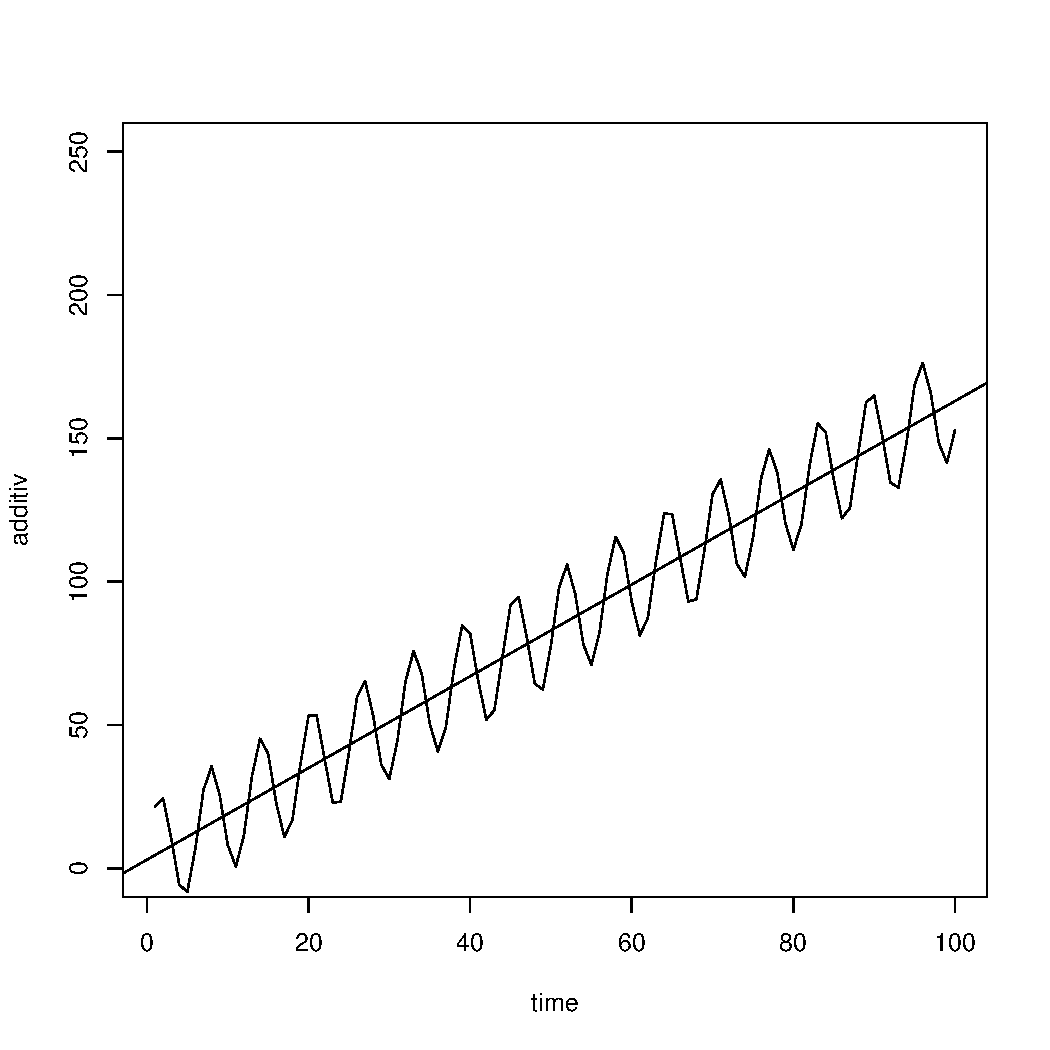
\includegraphics[width = .45\textwidth]{figures/additiv.pdf}
        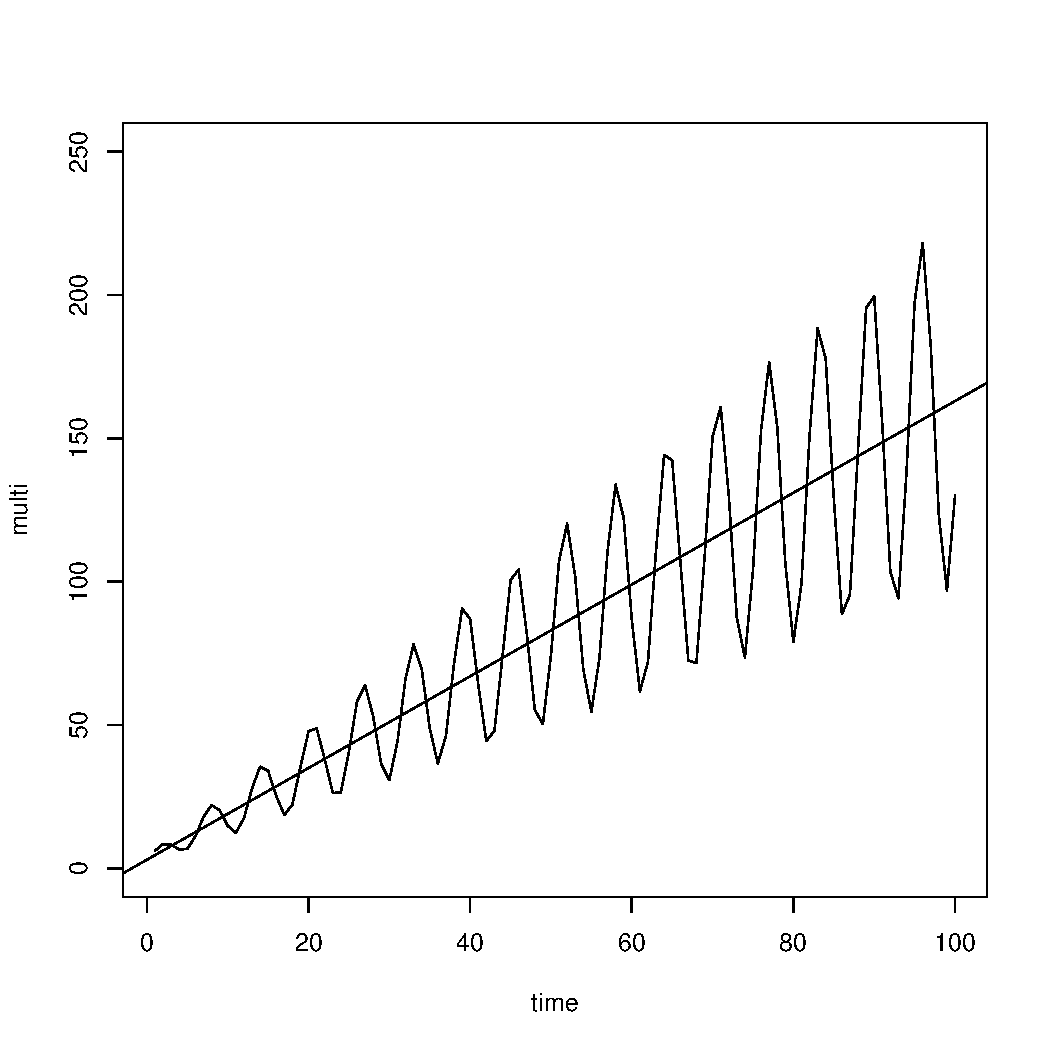
\includegraphics[width = .45\textwidth]{figures/multiplikativ.pdf}
    \caption{Schaubild für einen additiven (links) bzw. multiplikativen (rechts) Zusammenhang von Trend- und Saisonkomponente}
    \label{fig:add_mult}
\end{figure}

\subsection{Gleitende Durchschnitte}
Gleitende Durchschnitte sind eine Methode um den Trend, also die glatte Komponente $g_t$, zu schätzen. Durch die Glättung filtert man dabei die saisonalen Schwankungen heraus.

\paragraph{Gleitende Durchschnitte ungerader Ordnung:} Um den Wert des gleitenden Durchschnitts für einen bestimmten Zeitpunkt $t$ zu berechnen, berechnet man das arithmetische Mittel (vgl. Kap. \ref{sec:arithm}) über $k$ Werte vor und $k$ Werte nach diesem Zeitpunkt $t$, sowie dem Wert $y_t$ selbst. Der Parameter $k$ gibt dabei an wie viele Werte vor und nach dem Wert $y_t$ jeweils in den gleitenden Durchschnitt Mit einfließen sollen. Da insgesamt $2 \cdot k + 1$ Werte mit einfließen, spricht man vom gleitenden Durchschnitt $(2k + 1)$-ter Ordnung.\\
\textbf{Beispiel:} Würde man jeweils $k = 3$ vor und nach dem Zeitpunkt $t$ mit einfließen lassen, so spräche man von einem gleitenden Durchschnitt 7. Ordnung. 

\paragraph{Gleitende Durchschnitte gerader Ordnung:} Soll eine gerade Anzahl $k$ an Werten in den gleitenden Durchschnitt mit einfließen, gestaltet sich die Berechnung ein klein wenig komplizierter, da man nun nicht mehr auf natürliche Art und Weise einen mittleren Wert hat wie oben. Daher bedient man sich hier des "Tricks", die Werte am Rand des gewählten Fensters nur mit halbem Gewicht in den Durchschnitt mit einfließen zu lassen. Somit kommt man auf eine gerade Zahl an "ganzen" Werten. Man berechnet also das arithmetische Mittel über je $k$ Werte vor und nach diesem Zeitpunkt $t$, sowie dem Wert $y_t$ selbst und gewichtet die äußersten Werte mit $\frac{1}{2}$.\\
\textbf{Beispiel:} Für $k = 2$ fließen fünf Werte in den Durchschnitt mit ein: Die äußersten Werte nur zur Hälfte, die jeweils direkten "Nachbarn" des Wertes $y_t$ ganz und der Wert $y_t$ selbst ebenfalls ganz. Somit kommt man schließlich auf 4 "ganze" Werte, daher gleitender Durchschnitt 4. Ordnung.\\

\noindent \dangersign Obwohl bei obigem Beispiel tatsächlich fünf Werte mit einfließen, wird bei der Berechnung des airthm. Mittels nur durch vier geteilt, da zwei Werte nur jeweils mit Gewicht $\frac{1}{2}$ einfließen.\\

\noindent Diese Berechnung führt man  für jeden Zeitpunkt $t$ der Zeitreihe durch und erhält damit eine geglättete Zeitreihe als Schätzung für die Trendkomponente. Wie man sich für eine Ordnung entscheidet, wird in den nachfolgenden Kapiteln erläutert.\\

\noindent \dangersign Je höher der gewählte Ordnung, für desto mehr Werte am Rand der Zeitreihe lässt sich kein gleitender Durchschnitt berechnen, da man immer $k$ Werte links \& rechts von dem Zeitpunkt $t$, für den man den gleitenden Durchschnitt berechnen will, braucht.\\

\noindent \framebox[\textwidth]{\texttt{R-Befehl für den gl. Durchschnitt: > runmean(data, k, ..)} \hfill \href{https://www.rdocumentation.org/packages/caTools/versions/1.17.1/topics/runmean}{Dokumentation}}

\noindent \dangersign Die R-Funktion ist \textbf{nicht} Teil von \texttt{base-R} sondern Teil des Paketes \texttt{caTools}. Dieses muss zunächst installiert (\texttt{install.packages("caTools")}) und anschließend importiert werden\\(\texttt{library(caTools)}).


\subsection{Saisonale Komponente, konstante Saisonfigur}
Gilt $s_t = s_{t+p}$, dann spricht man von einer konstanten Saisonfigur mit Periode $p$, da nach $p$ Zeitpunkten die Saisonkomponente wieder in etwa den gleichen Wert annimmt. Summiert man alle Werte dazwischenliegenden Werte dieser Periode auf, so sollte 0 herauskommen.\\

\noindent \dangersign Auch die Periodendauer $p$ ist etwas, das man durch grafische Darstellung der Zeitreihe herausfinden kann. Man überprüft visuell, ob es saisonale Muster gibt, die sich in regelmäßigen Zeitabständen wiederholen.

\subsection{Zerlegung in Trend und Saison}
Die saisonale Komponente ist "\textit{eine regelmäßige Wiederholende Schwankung um die glatte Komponente}". Wenn man daher die Ordnung des gleitenden Durchschnitts so wählt, dass sie einem Vielfachen $l$ der Periodendauer entspricht ($2k = l \cdotp p$, kann man die Zeitreihe "glätten", also die Saisonkomponente herausrechnen. Übrig bleibt dadurch eine Schätzung für die Trendkomponente $g_t$.
Die kleinste mögliche Ordnung um die Saisonkomponente zu eliminieren enstpricht somit der Periodendauer $p$.\\

\noindent \dangersign Höhere Ordnungen $l \cdot p$ sind theoretisch auch möglich (s.o.), würden jedoch dazu führen, dass man für mehr Zeitpunkte am Rand der Reihe keinen gleitenden Durchschnitt berechnen könnte.\\

\noindent Die Differenz $d_t$ zwischen dem urspr. Wert $y_t$ und geschätzten Trendkomponente $g_t$ entspricht bereits grob den saisonale Abweichungen, allerdings noch mit zusätzlichem Fehler.\\
Durch diese Berechnung der Differenzen erhalten wir nun für jeden Teil der Saisonfigur (bspw. für jedes Quartal) \textit{mehrere} Abweichungen (da in der Zeitreihe z.B. 8 mal ein erstes Quartal auftaucht) für die gilt, dass $d_t\approx d_{t+p}$. Daher mitteln wir für jeden Teil des Saisonfigur alle berechneten Abweichungen, die diesem Teil zuzuordnen sind (bspw. alle $d_t$ die für ein erster Quartal berechnet wurden). Dies führt zu Mittelwerten für jeden der $p$ Teile der Saisonkomponente: $(\bar{d}_1, \hdots, \bar{d}_p)$\\
Da die Summe über alle Teile der Saisonkomponente gleich Null sein muss, müssen diese Mittelwerte noch um die Null zentriert werden: Der Mittelwert der Teile $\bar{d}_1, \hdots, \bar{d}_p$, wird von allen Teilen $(\bar{d}_1, \hdots, \bar{d}_p)$ subtrahiert. Übrig bleibt dadurch die geschätzte Saisonkomponente $\hat{s}$.

\subsubsection{Trend und Saisonkomponente mit Regression}
Eine andere Möglichkeit der Trendschätzung ist die lineaere Regression (vgl. Kap. \ref{chap:linreg}). Nimmt man die Zeit $t$ als Einfluss- und die Zeitreihe $y_t$ als Zielgröße können hierdurch z.B. lineare quadratische Trends geschätzt werden. Ein Modell für die Trendkomponente könnte z.B. folgende Form haben: 
$$y_t=\hat{a}+\hat{b}\cdot t + e_t$$
\noindent Mittels eines multiplen Regressionsmodells (vgl. Kap. \ref{sec:mult-reg}, Statistik II) könnte simultan auch die Saisonkomponente geschätzt werden. Man nimmt dabei zusätzlich zu der Zeit $t$ Dummyvariablen (vgl. Kap. \ref{sec:kat-reg}) für jeden der $p$ Teile der Saisonfigur mit in das Modell auf. Dies führt schlussendlich zu folgendem Trend-Saison-Modell:
$$y_t=a + b \cdot t + \gamma_1 s_1(t) + \hdots + \gamma_{p} s_{p}(t) + e_t$$

\subsection{Alternative Ansätze}
Es gibt noch viele weitere (fortgeschrittenere) Ansätze wie Zeitreihen analysiert \& modelliert werden können, die jedoch den Umfang \& Schwierigkeitsgrad dieser Veranstaltung sprengen würden. Daher nur ein bisschen Name-Dropping:
\begin{itemize}
    \item Das lokale lineare Trendmodell
    \item Einbeziehung von trigonometrische Funktionen
    \item Census X-11 ARIMA
    \item Census X-12 ARIMA
    \item BV 4.1
\end{itemize}

Zu Zeitreihen gibt es eigene ganze Vorlesungen, siehe z.B.:

\begin{itemize}
    \item \href{https://www.finmetrics.statistik.uni-muenchen.de/studium_lehre/sommersemester-2020/tsa_19/index.html}{Time series analysis}
    \item \href{https://www.finmetrics.statistik.uni-muenchen.de/studium_lehre/sommersemester-2020/mtsa_2020/index.html}{Multivariate time series analysis}
\end{itemize}

\clearpage

\subsection{Aufgaben}

\paragraph{1. Welche Aussagen bzgl. gleitender Durchschnitte sind wahr?}

\begin{itemize}
    \item[a)] Durch k wird festgelegt, ob der die Ordnung der gl. Durchschnitt gerade oder ungerade\\ist. \hfill $\square$
    \item[b)] Bei einem gl. Durchschnitt ungerader Ordnung fallen am Rand der Zeitreihe mehr\\Werte weg als bei gerader Ordnung. \hfill $\square$
    \item[c)] Je höher die Ordnung, desto mehr Werte fallen am Rand der Zeitreihe weg. \hfill $\square$
    \item[d)] Bei einem gl. Durchschnitt gerader Ordnung gehen (bei gleichem k) mehr Werte\\in die Berechnung mit ein als bei ungerader Ordnung. \hfill $\square$
\end{itemize}

\paragraph{2. Welche Aussagen bzgl. des Zeitreihenmodells sind wahr?}

\begin{itemize}
    \item[a)] Mit gleitenden Durchschnitten kann die Trendkomponente geschätzt werden. \hfill $\square$
    \item[b)] Mit gleitenden Durchschnitten kann die Saisonkomponente geschätzt werden. \hfill $\square$
    \item[c)] Jede Zeitreihe besitzt eine Trend- und eine Saisonkomponente. \hfill $\square$
    \item[d)] Welche Ordnung für die gleitenden Durchschnitte gewählt wird, hängt von der\\Saisonkomponente ab. \hfill $\square$
\end{itemize}


\clearpage

%%%%%%%%%%%%%%%%%%%%%%%%%%%%%%%%%%%%%
%%%%%%%%%%  KAPITEL 10
%%%%%%%%%%%%%%%%%%%%%%%%%%%%%%%%%%%%%

\section{R-Einführung Teil I}

Teil der Veranstaltung ist eine Einführung in \texttt{R} sowie eine Computervorlesung. Dieses Kapitel dient als Platzhalter, falls in diesem Skript in Zukunft der Inhalt aus diesem Vorlesungskapitel vertieft werden sollte. Bis dahin wird empfohlen mit den vorhandenen Vorlesungsmaterialien zu arbeiten, da diese bereits sehr ausführlich und weitestgehend selbsterklärend sind.

\clearpage

\hspace{0pt}
\vfill
\begin{center}
    {\Huge Statistik II}
\end{center}
\vfill
\hspace{0pt}


\clearpage

%%%%%%%%%%%%%%%%%%%%%%%%%%%%%%%%%%%%%
%%%%%%%%%%  KAPITEL 11
%%%%%%%%%%%%%%%%%%%%%%%%%%%%%%%%%%%%%

\section{Kombinatorik}

Grundlegend ist hier zunächst mal die Unterscheidung von \textbf{Permutation} \& \textbf{Kombination}.
Unter der \textbf{Permutation} versteht man eine Möglichkeit, die $n$ Elemente einer Menge $M$ anzuordnen. Von einer \textbf{Kombination} spricht man, wenn man nicht (zwingend) alle $n$ Elemente auswählt. Formal ist eine Kombination eine "Möglichkeiten, $m$ Elemente aus $n$ Elementen einer Menge $M$ auszuwählen".\\
In beiden Fällen interessiert man sich für die \textit{Anzahl aller möglichen Permutationen/Kombinationen}.

\subsection{Permutation}\label{sec:perm}
Da bei der Permutation \textit{alle} Elemente ausgewählt \& angeordnet werden, spielt die Reihenfolge per Definition eine Rolle. Man unterscheidet jedoch die Fälle \textit{mit Wiederholung} und \textit{ohne Wiederholung}. Der Begriff \textit{Wiederholung} meint hier, ob ein Element nur einmal oder mehrfach angeordnet werden kann.\\
\textbf{Beispiel:} Wir möchten die Anzahl der verschiedenen Sitzordnungen im Hörsaal bestimmen.
\begin{itemize}
    \item[a)] Zunächst handelt es sich hier (natürlicherweise) um eine Permutation \textit{ohne Wiederholung}, da \textit{alle} Studierenden angeordnet werden und \textit{niemand zwei Plätze einnehmen kann}.
    \item[b)] Unterscheiden wir jedoch nicht jeden einzelnen Studierenden, sondern differenzieren nur nach Studienfach (z.B: \textit{BWL, VWL, Sonstiges}) erzeugen wir den Fall mit Wiederholung. Nun können mehrere Plätze durch z.B. Studierende der VWL eingenommen werden.
\end{itemize}
Stellt man sich diese Szenarien als Urnen-Experiment vor, so sind im Fall a) z.B. 100 Kugeln in der Urne (also eine pro Studierendem), welche alle angeordnet werden. Im Fall b) wären nur drei Kugeln in der Urne (eine pro Studienfach), welche nach dem Ziehen stets zurückgelegt werden müssten. \textit{Anmerkung:} Zurücklegen nur so oft, wie wir Studierende je Studienfach haben.

\subsubsection{Anzahl Permutationen ohne Wiederholungen}\label{sec:perm-ohne}
Stellt man sich dies als Baumdiagramm vor, so entstehen für die erste Stufe $n$ verschiedene Pfade, für die zweite Stufe jeweils nur noch $n-1$ (da bereits ein Element angeordnet wurde), für die dritte Stufe jeweils $n-2$, usw. So geht es weiter bis auf der letzten Stufe jeweils nur noch ein Pfad möglich ist.\\
Um die Gesamtzahl der möglichen Pfade zu erhalten, muss man die Anzahlen je Stufe miteinander multiplizieren: 
$$n \cdot (n-1) \cdot (n-2) \cdot \hdots \cdot 1 = n! \qquad \mbox{(ausgesprochen: n \textit{Fakultät})}$$

\noindent \framebox[\textwidth]{\texttt{R-Befehl für Fakultät: > factorial(x)} \hfill \href{https://www.rdocumentation.org/packages/base/versions/3.6.2/topics/Special}{Dokumentation}}

\subsubsection{Permutation mit Wiederholungen}\label{sec:perm-mit}
Bei der Permutation mit Wiederholungen sind nicht mehr alle Elemente unterschiedlich. Daher gibt es (bei gleichem $n$) hier nun eine geringere Zahl möglicher Permutationen, da es bei einem gleichen Element egal ist, ob die Elemente z.B. auf Platz 3 und 4 oder auf Platz 4 und 3 sind. Somit dürfen solche beispielhaften Anordnungen nicht mehr doppelt gezählt werden, sondern müssen "herausgerechnet" werden.\\
Deshalb teilt man $n!$ durch das Produkt der $n_i!$ verschiedenen Gruppengrößen:
$$\frac{n!}{n_1!\cdot n_2!\cdot...\cdot n_s!}$$

\noindent Mit $n_i$ berechnet man die Anzahl der möglichen Permutationen in der $i$-ten Gruppe. Da diese hier nicht mehr von Relevanz sind, werden sie herausgerechnet.

\subsection{Kombination}
Bei der Kombination werden \textbf{nicht mehr} alle $n$ Elemente aus $M$, sondern nur noch $m$ ausgewählt. Neben der Frage, ob eine Wiederholung möglich ist oder nicht, muss man sich daher hier auch die Frage stellen, ob die Reihenfolge bei der Auswahl eine Rolle spielt oder nicht. \\
\textbf{Beispiel:} Erweiterung des Beispiels aus Kapitel \ref{sec:perm}.
\begin{itemize}
    \item[a)] \textit{Ohne Wiederholung, ohne Reihenfolge:} Wie viele Möglichkeiten gibt es, 10 aus den 100 Studierenden auszuwählen.
    \item[a)] \textit{Ohne Wiederholung, mit Reihenfolge:} Wie viele Möglichkeiten gibt es, 10 der 100 Studierenden der Reihe nach auf den Plätzen in der ersten Reihe anzuordnen.
    \item[c)] \textit{Mit Wiederholung, ohne Reihenfolge:} Wie viele Möglichkeiten gibt es, 10 aus den 150 Studierenden (jedoch nur unterschieden nach Studienfach, s.o.) auszuwählen.
    \item[d)] \textit{Mit Wiederholung, Mit Reihenfolge:} Wie viele Möglichkeiten gibt es, 10 der 150 Studierenden (jedoch nur unterschieden nach Studienfach, s.o.) der Reihe nach auf den Plätzen in der ersten Reihe anzuordnen.
\end{itemize}
Stellt man sich diese Szenarien als Urnen-Experiment vor, so sind im Fall a) \& b) je 100 Kugeln in der Urne (also eine pro Studierendem), von denen in beiden Fällen 10 Stück gezogen werden. Im Fall a) interessiert man sich nicht für die Reihenfolge, in der man die Kugeln zieht, in Fall b) schon. Im Fall c) \& d) wären wieder nur drei Kugeln in der Urne (eine pro Studienfach), welche nach dem Ziehen stets zurückgelegt werden müssten. Im Fall c) interessiert man sich nicht für die Reihenfolge, in der man die Kugeln zieht, in Fall d) schon.\\

\noindent \dangersign Bei Permutationen wird die Anzahl der möglichen Permutationen durch Wiederholungen geringer, bei Kombinationen wird die Anzahl der möglichen Kombinationen, sowohl für den Fall mit, als auch für den Fall ohne, Berücksichtigung der Reihenfolge, durch Wiederholungen größer.

\clearpage

\subsubsection{Kombination ohne Wiederholung und ohne Reihenfolge}
Die Anzahl an möglichen Kombinationen berechnet man mit $\binom{n}{m}$. Da es keine Wiederholungen gibt ist in diesem Fall $m$ immer kleiner als $n$. Im Taschenrechner kann man den Binomialkoeffizient (so heißt die Funktion) mit \textit{nCr} berechnen z.B. 24nCr3 = $\binom{24}{3}$.\\
Man kann den Binomialkoeffizient auch als Permutation mit Wiederholung umschreiben, da man zwei Gruppen hat, zum einen die Gruppe mit den gezogenen Elementen $m$ und die Gruppe $n-m$  mit den nicht gezogenen Elementen. Somit ergibt sich: $$\binom{n}{m}=\frac{n!}{m!\cdot(n-m)!}$$

\noindent \framebox[\textwidth]{\texttt{R-Befehl für Fakultät: > choose(n, k)} \hfill \href{https://www.rdocumentation.org/packages/base/versions/3.6.2/topics/Special}{Dokumentation}}

\subsubsection{Kombination ohne Wiederholung und mit Reihenfolge}
Dieser Fall ist sehr nahe an \textit{Permutation ohne Wiederholung} (vgl. Kap. \ref{sec:perm-ohne}), der einzige Unterschied liegt darin, dass das Baumdiagramm nicht "fertig" gezeichnet wird (sondern nach $m$ Stufen abbricht). Multipliziert man den Binomialkoeffizient mit $m!$, so erhält man die passende Formel dafür: 
$$m! \cdot \binom{n}{m} = m! \cdot \frac{n!}{m!(n-m)!} = \frac{n!}{(n-m)!}$$ 

\noindent \dangersign Die Formel sieht komplizierter aus, als sie letztendlich ist. Im Grund steht im Nenner die Anzahl der nicht ausgewählten Elemente und kürzt dadurch den hinteren Teil von $n!$ weg, sodass diese nach $m$ Stufen abbricht.

\subsubsection{Kombination mit Wiederholung und ohne Reihenfolge}
Hier kann die Anzahl der ausgewählten Elemente $m$ größer sein als $n$, da mit Wiederholung gezogen wird. Zusätzlich zum Fall der Kombination ohne Wiederholung vergrößert man künstlich die Menge um $m-1$ Elemente. Dadurch wird nicht aus $n$, sondern aus $n+m-1$ Elementen gezogen:
$$\binom{n+m-1}{m}=\frac{(n+m-1)!}{m!(n-1)!}$$

\noindent \dangersign Diese Formel mag etwas komisch wirken, eine gute Intuition vermittelt jedoch das Beispiel mit den Eiskugeln aus dem Skript.

\subsubsection{Kombination mit Wiederholung und mit Reihenfolge}
Betrachtet man diesen Fall wieder als Baumdiagramm, so erhält man einen Baum mit $m$ Stufen und jeweils $n$ Pfaden pro Stufe. Man berechnet die Anzahl der möglichen Kombinationen durch $$n^m\;.$$

\clearpage

\subsection{Aufgaben}
\paragraph{1. Welche Aussagen bzgl. Permutationen sind wahr?}
\begin{itemize}
    \item[a)] Die Reihenfolge der Elemente kann eine Rolle spielen, muss es aber nicht. \hfill $\square$
    \item[b)] Permutation wird eine mögliche Anordnung von Elementen in einer bestimmten\\ Reihenfolge genannt.  \hfill $\square$
    \item[c)] Die Anzahl der Permutationen ohne Reihenfolge und ohne Wiederholung berechnet\\ man mit $n!$ \hfill $\square$
    \item[d)] Die Anzahl der möglichen Permutation mit Wiederholung ist größer als ohne\\ Wiederholungen. \hfill $\square$
\end{itemize}

\paragraph{2. Welche Aussagen bzgl. Kombinationen sind richtig?}
\begin{itemize}
    \item [a)] Die Betrachtung \textit{ohne Wiederholung und ohne Reihenfolge} hat eine größere Anzahl \\ an Kombinationsmöglichkeiten als die Betrachtung \textit{mit Wiederholung und ohne \\Reihenfolge.} \hfill $\square$
    \item[b)] Wenn die Reihenfolge bei der Kombination mit einbezogen werden soll, dann wird die \\Anzahl an möglichen Kombinationen größer.\hfill $\square$
    \item[c)] Bei Betrachtung von Kombinationen \textit{ohne Wiederholung und mit Reihenfolge} erhält\\ man eine höhere Anzahl an Möglichkeiten als bei der Permutation ohne Wiederholung \hfill $\square$
    \item[d)] Bei der Kombination mit Wiederholung und mit Reihenfolge gibt es auf dem \\"ersten Platz" $n$ verschiedene Möglichkeiten, auf dem "zweiten Platz" $n-1$, usw. \hfill $\square$
\end{itemize}

\paragraph{3. Ein Zahlenschloss besteht aus 4 Rädern mit den Zahlen von 0 bis 9. Welche Aussage ist richtig?}
\begin{itemize}
    \item[a)] Um die Anzahl der möglichen Kombinationen zu berechnen benutzt man die\\ Permutation mit Wiederholung.\hfill $\square$
    \item[b)] Um die Anzahl der möglichen Kombinationen zu berechnen benutzt man die\\ Kombination mit Wiederholung und mit Reihenfolge.\hfill $\square$
    \item[c)] Um die Anzahl der möglichen Kombinationen zu berechnen benutzt man die\\ Kombination mit Wiederholung und ohne Reihenfolge.\hfill $\square$
    \item[d)] Um die Anzahl der möglichen Kombinationen zu berechnen benutzt man die\\ Kombination ohne Wiederholung und ohne Reihenfolge.\hfill $\square$
    \item[e)] Es gibt 10.000 verschiedene Kombinationen.\hfill $\square$
\end{itemize}

\paragraph{4. Bei einem Basketballspiel laufen nacheinander 5 Spieler auf das Spielfeld. Man berechnet die Anzahl der Möglichkeiten für das Einlaufen mit ...}
\begin{itemize}
    \item[a)] der Kombination ohne Wiederholung und mit Reihenfolge.\hfill $\square$
    \item[b)] der Permutation ohne Wiederholung.\hfill $\square$
    \item[c)] der Permutation mit Wiederholung.\hfill $\square$
    \item[d)] der Kombination ohne Wiederholung und ohne Reihenfolge.\hfill $\square$
    \item[e)] der Kombination mit Wiederholung und mit Reihenfolge.\hfill $\square$
\end{itemize}

\paragraph{5. Bei einem Rosenzüchter gibt es 14 verschiedene Rosenarten und man möchte ein Strauß mit 20 Rosen. Wie viele unterschiedliche mögliche Sträuße gibt es?}
\begin{itemize}
    \item[a)] $2,432902008 \times 10^{18}$ \hfill $\square$
    \item[b)] $5,73166440 \times 10^8$ \hfill $\square$
    \item[c)] $8,366825543 \times 10^{22}$ \hfill $\square$
    \item[d)] $8,71782912 \times 10^{10}$ \hfill $\square$
\end{itemize}


\clearpage

%%%%%%%%%%%%%%%%%%%%%%%%%%%%%%%%%%%%%
%%%%%%%%%%  KAPITEL 12
%%%%%%%%%%%%%%%%%%%%%%%%%%%%%%%%%%%%%

\section{Wahrscheinlichkeitsrechnung}\label{chap:wkeit}
\subsection{Grundlagen \& -begriffe}\label{sec:wkeit-basics}
Zunächst ein paar Begriffserklräungen, für das bessere Verständnis:
\paragraph{Ein Elementarereignis} ist ein Ereignis, desen Menge nur aus einem Element besteht (z.B. bei einem Münzwurf: \textit{Kopf} bzw. \textit{Zahl}). Ein \textbf{zufälliges Ereignis} ist die Kombination mehrerer Elementarereignisse (z.B. beim Würfel: \textit{Gerade Zahl würfeln} = $\{2,4,6\}$).
\paragraph{Der Ereignisraum} $\Omega$ ist die Menge aller Elementarereignisse (z.B. bei einem Münzwurf die Menge $\{Kopf,\; Zahl\}$).
\paragraph{Ein unmögliches Ereignis} ist ein Ereignis, dass kein Elementarereignis enthält (z.B. beim Münzwurf $\{Kreuz\}$ oder $\{Pik\}$), ein \textbf{sichere Ereignis} hingegen enthält alle möglichen Elementarereignisse (also $\Omega$).\\

\noindent Zufällige Ereignisse können nicht nur alleine auftreten, da diese Mengen von Elementarereignissen sind. Zur Verknüpfung benötigt man sog. Mengenoperation:

\paragraph{A geschnitten B} [$A\; \cap\; B$]\; Dies ist die \textit{Schnittmenge} der beiden Mengen $A$ und $B$, d.h. diejenigen Elementarereignisse, die sowohl in $A$ \textit{als auch} auch in $B$ enthalten sind. Ist $A\cup B=\emptyset$ (d.h. die Schnittmenge ist leer), so spricht man von \textbf{disjunkten Ereignissen}. 

\paragraph{A vereinigt B} [$A\; \cup\; B$]\; Dies ist die Vereinigungsmenge, d.h. alle Elementarereignisse, die entweder in $A$ \textit{oder} in $B$ (oder in beiden) enthalten ist. Hierfür werden beide Mengen addiert, wobei Elementarereignisse, die in beiden Mengen vorkommen, nur einmal gezählt werden dürfen.

\paragraph{Nicht A} [$\bar A$]\; Das zufällige Ereignis $\bar A$ (sprich: \textit{A quer}) enthält ausschließlich diejenigen Elementarereignisse, welche in $A$ enthalten sind.

\paragraph{A ohne B} [$A\; \setminus\; B$]\; Die Ereignis bezeichnet alle Elementarereignisse, welche in $A$, jedoch nicht in $B$ enthalten sind. $B\; \setminus\; A$ wären alle, die in $B$, jedoch nicht in $A$ enthalten sind.


\subsection{Relative Häufigkeit}
Um (ohne theoretisches Vorwissen) eine Quantifizierung vorzunehmen, wie häufig ein Ereignis zu erwarten ist bzw. wie wahrscheinlich der Ausgang eines Versuchsergebnisses ist, betrachtet man relative Häufigkeiten (vgl. Kap. \ref{sec:rel-hkeit}).
Zieht man dabei ausreichend viele Wiederholungen des Zufallsexperiments heran, so nähert sich die relative Häufigkeit der Wahrscheinlichkeit von $A$ an. Diese wird als $P(A)$ geschrieben.

\subsection{Laplacesche Wahrscheinlichkeit}\label{sec:laplace}
Als Laplace-Experiment bezeichnet man ein Zufallsexperiment, bei dem alle Elementearereignisse die gleiche Wahrscheinlichkeit besitzen (\& der Ereignisraum endlich ist). Dadurch kann man z.B. die Wahrscheinlichkeit für Ereignis $A$ berechnetn, indem man einfach den Quotient aus der Anzahl der für $A$ günstigen Fälle und der Anzahl aller möglichen Elementarereignisse bilden: $\frac{|A|}{|\Omega|}=P(A)$.\\
\textbf{Beispiel:} Der Würfelwurf ist ein Laplace-Experiment, da jede Zahl die gleiche Wahrscheinlichkeit von $\frac{1}{6}$ besitzt und somit z.B. $P(gerade\; Zahl) = \frac{3}{6}$ berechnet werden kann.

\subsection{Axiome} \label{sec:axiome}
Das Axiomensystem von Kolmogorov bietet die formale Grundlage für die Wahrscheinlichkeitsrechnung und besteht aus drei Axiomen.

\paragraph{1. Axiom:} Jede Wahrscheinlichkeit liegt zwischen 0 und 1.

\paragraph{2. Axiom:} Die Wahrscheinlichkeit für das sichere Ereignis (vgl. Kap. \ref{sec:wkeit-basics}) beträgt 1.

\paragraph{3. Axiom:} Die Wahrscheinlichkeiten zweier disjunkter Ereignisse können einfach addiert werden um die Wahrscheinlichkeit der Vereinigungsmenge zu bestimmen.

\paragraph{Folgerungen:}
Aus diesen Axiomen lassen sich 5 Folgerungen ableiten:
\begin{enumerate}
    \item W'keit des Komplementärereignisses: $P(\bar A) = 1 - P(A)$, da $A \cup \bar A = \Omega$
    \item W'keit des unmöglichen Ereignisses: $P(\emptyset) = 0$, da $\emptyset = \bar \Omega$ \& $P(\Omega) = 1$
    \item W'keit der Vereinigungsmenge: $P(A \cup B) = P(A) + P(B) - P(A \cap B)$, da die Schnittmenge sowohl in P(A), als auch in P(B) reinspielt \& sonst quasi "doppelt" zählen würde.\\
    \dangersign Sind $A$ \& $B$ disjunkt, reduziert sich dies auf das dritte Axiom, da $P(A \cap B) = 0$
    \item W'keit der Teilmenge: Wenn $A$ Teilmenge von $B$ ist, so gilt: $P(A) \leq P(B)$
    \item Kann man $\Omega$ vollständig in disjunkte Teile $A_1,....,A_n$ zerlegen, so gilt für Ereignis $B$:\\$P(B) = \sum_{i=1}^n P(B \cap A_i)$, d.h. $P(B)$ kann vollständig in die W'keiten der Schnittmengen mit den $A_i$ zerlegt werden.
\end{enumerate}

\subsection{Bedingte Wahrscheinlichkeit}\label{sec:bed-wkeit}
Bei der bedingten Wahrscheinlichkeit handelt es sich um eine Wahrscheinlichkeit eines Ereignisses $B$, bei der schon als Vorinformation bekannt ist, dass ein Ereignis $A$ bereits eingetreten ist. Nun ist die Frage, ob das eingetretene Ereignis $A$ eine Auswirkung auf  $P(B)$ hat und wie man diese Auswirkung bei der Berechnung von $P(B)$ berücksichtig. Formal schreibt man diese sog. \textbf{bedingte Wahrscheinlichkeit} als $P(B|A)$.\\
Man berechnet sie aus dem Quotient der Wahrscheinlichkeit der Schnittmenge (in diesem Fall von $A$ und $B$) und der Wahrscheinlichkeit für die Bedingung, also hier von $P(A)$.
$$P(B|A)=\frac{P(A \cap B)}{P(A)}$$

\noindent \dangersign Andersherum funktioniert es natürlich genauso, d.h. $P(A|B) = \frac{P(A \cap B)}{P(B)}$\\

\noindent Stellt man diese Formel nach der gemeinsamen Wahrscheinlichkeit um, so ergibt sich der sog. \textbf{Multiplikationssatz}:
$$P(A \cap B) = P(B|A) \cdot P(A) \qquad bzw: \qquad P(A \cap B) = P(A|B) \cdot P(B)$$

\noindent Die bedingt Wahrscheinlichkeit, sowie deren Umformung, sind von zentraler Bedeutung für die Herleitung der nächsten beiden Sätze.

\subsubsection{Satz von der totalen Wahrscheinlichkeit}\label{sec:tot-wkeit}
Möchte man eine Wahrscheinlichkeit eines Ereignisses berechnen, kann man den Satz der totalen Wahrscheinlichkeit verwenden. Grundlage ist Folgerung 5 aus Kapitel \ref{sec:axiome}, in der man die Wahrscheinlichkeit des Ereignisses $B$ als Summe der Wahrscheinlichkeiten der Schnittmengen von $B$ mit jedem disjunkt zerlegten Teil $A_i$ des Ereignisraumes $\Omega$ berechnet.\\
Da die Wahrscheinlichkeit der Schnittmenge auch durch bedingten Wahrscheinlichkeiten berechnet werden kann, setzt man das Produkt aus jeder bedingten Wahrscheinlichkeit von $B$ unter der Bedingung $A_i$ ein \& multipliziert dies jeweils mit der Wahrscheinlichkeit der Vorinformation $A_i$. Anschließend werden diese Produkte (wie in Folgerung 5) aufsummiert, um so die Wahrscheinlichkeit für das Ereignis $B$ zu erhalten:
$$P(B) = \sum_{i=1}^n P(B \cap A_i) = \sum_{i=1}^n P(B|A_i) \cdot P(A_i)$$

\subsubsection{Der Satz von Bayes}\label{sec:bayes}
Den Satz von Bayes wird verwendet, um eine bedingte Wahrscheinlichkeit zu berechnen. Verwendet man beide Versionen des Multiplikationssatzes und setzt diese über die gemeinsame Wahrscheinlichkeit gleich, so erhält man: 
$$P(B|A) \cdot P(A) = P(A|B) \cdot P(B)$$

\noindent Umgestellt nach einer der beiden bedingten Wahrscheinlichkeiten ergibt sich:
$$ P(A|B) = \frac{P(B|A)\cdot P(A)}{P(B)} \qquad bzw: \qquad P(B|A) = \frac{P(A|B)\cdot P(B)}{P(A)}$$

\noindent \dangersign Ist eine \textbf{unbedingte Wahrscheinlichkeit} gesucht, so ist meistens der Satz der totalen Wahrscheinlichkeit hilfreich, sucht man eine \textbf{bedingt Wahrscheinlichkeit} so benötigt man meist den Satz von Bayes

\clearpage 

\subsection{Stochastische Unabhängigkeit}\label{sec:sto-unabh}
Stochastische Unabhängigkeit liegt vor, wenn die bedingte Wahrscheinlichkeit eines Ergeignisses gleich der unbedingten Wahrscheinlichkeit ist, d.h. $P(B) = P(B|A)$. Dies bedeutet, dass das Eintreten eines Ereignisses $A$ kein Einfluss auf die Wahrscheinlichkeit für das Eintreten eines Ereignisses $B$ hat. Grob gesagt heißt das: Egal ob das Ereignis $A$ eintritt oder nicht, weiß ich immer noch nicht mehr über die Wahrscheinlichkeit des Eintreten des Ereignisses $B$ als davor. Die Intuition ist dabei ähnlich zu der in Kapitel \ref{sec:unabh}, jedoch beziehet sich diese Begriff auf \textit{Wahrscheinlichkeiten} und nicht mehr auf \textit{relative Häufigkeiten} (daher auch \textit{stochastische} Unabhängigkeit).
Überprüfbar ist stochastische Unabhängigkeit zwischen zwei Ereignissen $A$ \& $B$ mittels
$$P(A \cap B) \stackrel{?}{=} P(A) \cdot P(B)\;.$$

\noindent Gilt diese Gleichung, so können $A$ \& $B$ als stochastisch unabhängig bezeichnet werden.

\clearpage

\subsection{Aufgaben}
\paragraph{1. Eine Mutter kauft für den Kindergeburtstag 20 Luftballons, 10 blaue und 10 rote. Welche Aussagen sind richtig?}
\begin{itemize}
    \item[a)] Ein sicheres Ereignis wäre entweder die Farbe blau oder rot als erstes aufzublasen.\hfill $\square$
    \item[b)] Ein unmögliches Ereignis wäre die Farbe gelb als erstes auszublasen. \hfill $\square$
    \item[c)] Das Komplementärereignis $\bar A$ von Ereignis $A$ "\textit{Einen blaue Luftballon als erstes \\aufblasen}" ist "\textit{Keinen Luftballon aufblasen}". \hfill  $\square$
    \item[d)] Bei der Frage, welchen Luftballon die Mutter als erstes aufbläst, gibt es hier zwei\\ Elementarereignisse. \hfill $\square$
    \item[e)] Das Ereignis "\textit{Blauen Luftballon als erstes aufblasen}" ist ein Elementarereignis. \hfill $\square$
\end{itemize}

\paragraph{2. Welche Aussagen zur Laplaceschen Wahrscheinlichkeit sind richtig?}
\begin{itemize}
    \item [a)] Bei der Laplaceschen Wahrscheinlichkeit kann der Ereignisraum unendlich sein,\\ solange die Ereignisse gleich wahrscheinlich sind. \hfill $\square$
    \item[b)] Die einzige Voraussetzung für ein Laplacesche Wahrscheinlichkeit ist, dass \\die Ereignisse gleich wahrscheinlich sind.\hfill $\square$
    \item[c)] Mit der Anzahl der für $A$ günstigen Fälle und der Anzahl aller möglichen\\ Ereignisse berechnet man die Laplacesche Wahrscheinlichkeit. \hfill $\square$
    \item[d)] Bei der Laplaceschen Wahrscheinlichkeit muss ein Zufallsexperiment zugrunde liegen. \hfill $\square$
\end{itemize}

\paragraph{3. Welche Aussagen zur Wahrscheinlichkeitsrechnung sind wahr?} 
\begin{itemize}
    \item[a)] Die Wahrscheinlichkeit eines unmöglichen Ereignisses ist die leere Menge. \hfill $\square$
    \item[b)] Die Wahrscheinlichkeit der Schnittmenge zweier disjunkter Ereignisse ist die Summe\\ der Einzelwahrscheinlichkeiten abzüglich der  Schnittmenge der beiden Ereignisse.\hfill $\square$
    \item[c)] Wenn man die Wahrscheinlichkeit des Ereignisses $A$ kennt, kann man auch die\\ Wahrscheinlichkeit des Komplementärereignisses $\bar A$ berechnen.\hfill $\square$
    \item[d)] Die Wahrscheinlichkeit eines Ereignisses $A$ kann Zahlen zwischen -1 und 1 annehmen.\hfill $\square$
    \item[e)] Ist $B$ eine Teilmenge von $A$, so ist die Wahrscheinlichkeit von $B$ kleiner oder \\gleich der Wahrscheinlichkeit von $A$. \hfill $\square$
\end{itemize}

\paragraph{4. Welche Aussagen zur bedingten Wahrscheinlichkeit sind wahr?}
\begin{itemize}
    \item[a)] Den Satz der totalen Wahrscheinlichkeit verwendet man, wenn man die \\unbedingte Wahrscheinlichkeit eines Ereignisses berechnen möchte. \hfill $\square$
    \item[b)] Man kann den Satz von Bayes verwenden, um eine bedingte Wahrscheinlichkeit\\ zu berechnen. \hfill $\square$
    \item[c)] Die bedingte Wahrscheinlichkeit $P(E|G)$ bedeutet die Wahrscheinlichkeit des\\ Ereignisses $E$, unter der Bedingung, dass das Ereignis $G$ nicht eintgereten ist. \hfill $\square$
    \item[d)] Wenn die bedingte Wahrscheinlichkeit $P(A|B)$ ungleich der bedingten\\Wahrscheinlichkeit $P(B|A)$, dann sind $A$ \& $B$ disjunkt. \hfill $\square$
\end{itemize}

\paragraph{5.Welche Aussagen zur stochastischen Unabhängigkeit sind wahr?}
\begin{itemize}
    \item[a)] Wenn die bedingte Wahrscheinlichkeit $P(A|B)$ ungleich der bedingten\\Wahrscheinlichkeit $P(B|A)$, dann sind $A$ \& $B$ unabhängig. \hfill $\square$
    \item[b)] Ist die bedingte Wahrscheinlichkeit $P(B|G)$ ungleich der Wahrscheinlichkeit $P(B|\bar G)$, \\dann liegt keine stochastische Unabhängigkeit zwischen B und G vor. \hfill $\square$
    \item[c)] Ist die bedingte Wahrscheinlichkeit $P(B|G)$ ungleich der Wahrscheinlichkeit $P(B)$, \\dann liegt keine stochastische Unabhängigkeit zwischen $B$ und $G$ vor. \hfill $\square$
    \item[d)] Liegt stochastische Unabhängigkeit vor, so berechnet man die gemeinsame\\ Wahrscheinlichkeit als die Summe der beiden Einzelwahrscheinlichkeiten. \hfill $\square$
\end{itemize}


\clearpage

%%%%%%%%%%%%%%%%%%%%%%%%%%%%%%%%%%%%%
%%%%%%%%%%  KAPITEL 13
%%%%%%%%%%%%%%%%%%%%%%%%%%%%%%%%%%%%%

\section{Zufallsvariablen}\label{chap:zv}

In der deskriptiven Statistik (Statistik I) haben wir fest vorgegebenes Datenmaterial beschrieben. Im Gegensatz dazu gehen wir in der induktiven Statistik (Statistik II) von Zufallsexperimenten mit sogenannten Zufallsvariablen aus. Mit Zufallsvariablen können Ergebnisse eines noch nicht durchgeführten Zufallsexperiments beschrieben werden.

\paragraph{Beispiel:} Roulette Spiel mit der Zufallsvariable $Z$ ("groß Z"): Bevor wir das Roulette drehen, ist der Wert von Z nicht bekannt, sondern nur Wahrscheinlichkeiten über die möglichen Ausprägungen. Nach einer Runde nimmt die Variable Z aber einen Wert zwischen $0,1,2,...,36$ an. Dieser Wert heißt auch Realisierung der Zufallsvariable und wird mit z ("klein z") beschrieben.

\noindent Grundsätzlich gibt es zwei verschiedene Arten von Zufallsvariablen -- \textbf{diskrete} und \textbf{stetige}. 

\subsection{Diskrete Zufallsvariablen} \label{sec:dzv}
Wenn Zufallsvariablen nur eine endliche oder abzählbar unendliche Menge an Werten annehmen, spricht man von diskreten Zufallsvariablen. Das bedeutet grob, dass es z.B. eine fixe Anzahl an Werten gibt (wie z.B. beim Roulette-Spiel oder Würfelwurf), oder dass es sich um sogennante Zähldaten handelt, wie etwa die Anzahl an Versicherungsschäden an einem bestimmten Tag. Jedoch ist zu beachten, dass theoretisch beliebig hohe Werte möglich sind, diese jedoch abzählbar sein müssen. 

\paragraph{Abzählbarkeit: Mächtigkeit von Mengen} Für Interessierte gibt es hier einen kleinen  \href{https://de.wikibooks.org/wiki/Mathe_f\%C3\%BCr_Nicht-Freaks:_M\%C3\%A4chtigkeit_von_Mengen}{Ausflug in die Mathematik}

\paragraph{Wahrscheinlichkeitsfunktion} Die Funktion $P(X = x_i= p_i$ ordnet jeder möglichen Ausprägung $x_i$ einer diskreten Zufallsvariable $X$ eine Wahrscheinlichkeit $p_i$ zu. (\textit{Anmerkung:} $\sum_{i=1}^n p_i = 1)$

\subsection{Stetige Zufallsvariablen} \label{sec:szv}
Stetige Zufallsvariablen sind innerhalb eines beliebigen Intervalls definiert und können unendlich viele verschiedene Werte annehmen. Man nennt diesen Wertebereich überabzählbar unendlich.

\paragraph{Beispiel:} Geschwindigkeit von Autos bei einer Radarkontrolle. Hier sind theoretisch unendlich viele Werte zwischen z.B. 50km/h und 60km/h möglich. Obwohl natürlich die Messgenauigkeit durch das verwendete Messgerät beschränkt ist (z.B. auf 1km/h genau), werden solche Variablen in der Statistik also meist als stetige Variablen behandelt.

\paragraph{Dichtefunktion} Das stetige Analogen zur Wahrscheinlichkeitsfunktion beschreibt stetige Zufallsvariablen. (\textit{Anmerkung: Muss stets $\geq$ 0 sein }\& $\int_{-\infty}^{\infty} f(x)\; dx = 1$)\\

\noindent \dangersign Bei stetigen Zufallsvariablen sind die Punktwahrscheinlichkeiten stets Null, d.h. wir könneen lediglich Aussagen über Wahrscheinlichkeiten für Intervalle treffen.

\subsection{Träger einer Zufallsvariablen} \label{sec:traeger}

Der Träger einer Zufallsvariablen bezeichnet alle möglichen Ergebnisse einer Zufallsvariablen. Beim Roulette-Spiel wäre der Träger z.B. $ T = 0,1,2,...,36$. Für die Geschwindigkeit bei der Radarkontrolle kommen theoretisch alle positiven reellen Zahlen in Frage, hier wäre der Träger also die Menge der reellen Zahlen $\R^+$.

\subsection{Verteilungsfunktion}\label{sec:vtlgfkt}

Die Interpretation ist relativ ähnlich zur empirischen Verteilungsfunktion aus Kapitel \ref{sec:emp-vert}, mit dem Unterschied, dass wir hier von \textit{Wahrscheinlichkeiten} anstatt von relativen Häufigkeiten sprechen. D.h. es handelt sich um ein rein theoretisches Konstrukt (im Gegensatz zum \textit{empirischen} Verteilungsfunktion).\\

\noindent \dangersign Bei diskreten Zufallsvariablen wird über die Punktwahrscheinlichkeiten aufsummiert ($\rightarrow$ Treppenfunktion), bei stetigen Zufallsvariablen über die Dichtefunktion integriert ($\rightarrow$ glatter Verlauf).

\subsection{Erwartungwert \& Varianz}\label{sec:ex-var}

Ähnlich der zentralen Lagemaße für \textit{Daten} in der deskriptiven Statistik (vgl. Kap. \ref{sec:median} oder \ref{sec:arithm}) dient der Erwartungswert zur Beschreibung des Schwerpunktes der Verteilung von \textit{Zufallsvariablen}. Die Varianz dient dazu, die Streuung von Verteilungen um deren Erwartungswert zu quantifizieren, im Gegensatz zur \textit{empirischen} Varianz (vgl. Kap. \ref{sec:varianz}) welche die Streuung von \textit{Daten} um deren Mittelwert quantifiziert.\\

\noindent \dangersign Auch hier ist bei der Berechnung wieder die Fallunterscheidung zwischen diskreten Zufallsvariablen (\textit{Summation}; eher simpel) und stetigen Zufallsvariablen (\textit{Integration}; eher aufwändig) nötig.

\subsection{Zweidimensionale Zufallsvariablen}\label{sec:2zv}

Zweidimensionale diskrete Verteilungen können über eine Kontingenztafel (vgl. Kap. \ref{sec:kont}) dargestellt werden, für den stetigen Fall Bedarf es einer gemeinsamen Dichtefunktion $f_{XY}(x,y)$.\\
Das Prinzip der Unabhängigkeit ist ähnlich definiert wie in Kapitel \ref{sec:unabh}, in diesem Fall jedoch wieder umgemünzt auf Wahrscheinlichkeiten anstatt relative Häufigkeiten. Ebenso einfach kann die Idee für die Kovarianz \& die Korrelation übertragen werden.

\clearpage

\subsection{Aufgaben}
\paragraph{Welche Aussagen zu den Zufallsvariablen sind richtig?}
\begin{itemize}
    \item[a)] Der fünffache Münzwurf ist eine diskrete Zufallsvariable. \hfill $\square$
    \item[b)] Mit Zufallsvariablen können Ergebnisse von Zufallsexperimenten beschrieben werden,\\ die noch nicht durchgeführt wurden. \hfill $\square$
    \item[c)] Der Träger der Zufallsvariable Würfelwurf eines 24-seitigen Würfels ist\\ $T = \{1, 2, 3, \hdots, 24\}$ \hfill $\square$
    \item[d)] Eine stetige Zufallsvariable hat abzählbar endlich viele mögliche Ergebnisse. \hfill $\square$
\end{itemize}

\clearpage

%%%%%%%%%%%%%%%%%%%%%%%%%%%%%%%%%%%%%
%%%%%%%%%%  KAPITEL 14
%%%%%%%%%%%%%%%%%%%%%%%%%%%%%%%%%%%%%

\section{Spezielle Verteilungen} \label{sec:Distr}

\subsection{Diskrete Verteilungen} \label{sec:discretedistr}
\paragraph{Diskret} heißt grob gesagt, dass ein Experiment eine endliche Zahl an möglichen Ergebnissen hat. Beispiele für diskrete Verteilungen in der Vorlesung sind die diskrete Gleichverteilung, Bernoulliverteilung, Binomialverteilung, (hyper--)geometrische Verteilung, Poissonverteilung und die Multinomialverteilung. Diese diskreten Verteilungen beschreiben Wahrscheinlichkeiten, mit denen die einzelnen Werte von diskreten Zufallsvariablen (=ZV) auftreten können. Diese ZV besitzt abzählbar viele Werte (Beispiel Würfelwurf mit den Zahlen 1--6).

\subsubsection{Diskrete Gleichverteilung} \label{sec:duni}

\paragraph{Idee/Anwendung:} Modellierung einer diskreten ZV, deren mögliche Ausprägungen alle mit derselben Wahrscheinlichkeit auftreten. 

\paragraph{Ein Beispiel} dafür ist das Würfeln mit einem fairen Würfel. \textit{Fair} bedeutet in diesem Fall, dass jede Augenzahl (das sind die möglichen Ausprägungen) mit derselben Wahrscheinlichkeit vorkommt.

\paragraph{Verteilung:} 
\begin{itemize}
\item[] Wahrscheinlichkeitsfunktion: $P(X=x_i)=p_i=\frac{1}{k}, \hspace{0.2cm} i=1,2,...,k$
	\begin{itemize}
	\item[$\rightarrow$] Hier ist die Wahrscheinlichkeitsfunktion an der Stelle $x_i$ einfach die Wahrscheinlichkeit, dass die ZV den Wert $x_i$ annimmt. Und diese Wahrscheinlichkeit ist für alle $x_i$, $i=1,2,...,k$, gleich und hat dementsprechend jeweils den Wert $\frac{1}{k}$.
	\end{itemize}
\item[] Erwartungswert und Varianz: $\E[X]=\frac{k+1}{2}$ und $Var[X]=\frac{1}{12}(k^2-1)$
\end{itemize}
\paragraph{Bemerkung:} $k$ ist die Anzahl der möglichen Ausprägungen, d.h. die Mächtigkeit des Ereignisraums\\

\noindent \framebox[\textwidth]{\texttt{R-Befehl für die diskerte Gleichverteilung: > \_dunif()}\\ \mbox{} \hfill \href{https://www.rdocumentation.org/packages/extraDistr/versions/1.8.11/topics/DiscreteUniform}{Dokumentation}}

\noindent \dangersign Für \textbf{alle} Verteilungen gibt es in \texttt{R} vier verschiedene mögliche Befehle, die durch einen Buchstaben vor dem Verteilungsnamen unterschieden werden (daher hier ein "\_" als Platzhalter. Ein \texttt{d} steht für die Dichte-/Wahrscheinlichkeitefunktion (\texttt{ddunif}), ein \texttt{p} für die Verteilungsfunktion (\texttt{pdunif}), ein \texttt{q} für die Quantilsfunktion (\texttt{qdunif}) und ein \texttt{r} für eine Zufallszahl (\texttt{rdunif})

\noindent \dangersign Die R-Funktionen sind \textbf{nicht} Teil von \texttt{base-R} sondern Teil des Paketes \texttt{extraDistr}. Dieses muss zunächst installiert (\texttt{install.packages("extraDistr")}) und anschließend importiert werden (\texttt{library(extraDistr)}).

\subsubsection{Bernoulliverteilung} \label{sec:Ber}

\paragraph{Idee/Anwendung:}  Ein einziges Experiment mit nur zwei möglichen Ergebnissen, wobei wir 0 für "Misserfolg" und 1 für "Erfolg" kodieren. Erfolg tritt mit Wahrscheinlichkeit $p$ und Misserfolg mit der entsprechenden Gegenwahrscheinlichkeit $(1-p)$ auf. Formell: $P(X=1)=p$ und $P(X=0)=1-p$. 

\paragraph{Ein Beispiel} ist der einfache Münzwurf einer fairen Münze. Hierbei spielt es keine Rolle, ob man Kopf oder Zahl als Erfolg (Misserfolg) wählt, es sei denn, man hat eine weitere, persönliche Interpretation der Ereignisse. Wenn man z.B. in einer Wette auf Kopf setzt, ist es sinnvoll, dem Ereignis $Kopf$ den Wert $1$, also "Erfolg", zuzuweisen.

\paragraph{Verteilung:}
\begin{itemize}
\item[] Notation: $X\sim B(1,p)$
\item[] Wahrscheinlichkeitsfunktion: $P(X=x) = \begin{cases}
			p & \text{für x = 1,}\\
            1-p & \text{für x = 0}
		 \end{cases}$ 
\item[] \hspace{4.5cm} bzw. $P(X=x)=p^x(1-p)^{1-x}$ für $x \in \{0,1\}$
	\begin{itemize}
	\item[$\rightarrow$] Wahrscheinlichkeitsfunktion nimmt für beide möglichen Werte (es handelt sich ja um eine binäre ZV) die entsprechende Eintrittswahrscheinlichkeit an. Ansonsten ist sie nicht definiert (was für uns so viel bedeutet, dass sie dort einfach "0" ist).
	\end{itemize}
\item[] Erwartungswert und Varianz: $\E[X]=p$ und $Var[X]=p(1-p)$
\end{itemize}

\paragraph{Bemerkung:} Binomialverteilung ($B(n,p)$) mit $n=1$.\\

\noindent \framebox[\textwidth]{\texttt{R-Befehl für die Bernoulliverteilung: > \_binom(.., size = 1)}\\ \mbox{} \hfill \href{https://www.rdocumentation.org/packages/stats/versions/3.6.2/topics/Binomial}{Dokumentation}}

\subsubsection{Binomialverteilung} \label{sec:Bin}

\paragraph{Idee/Anwendung:} Die Binomialverteilung entsteht durch mehrmaliges ($n$--maliges) Wiederholen desselben Bernoulli-Experiments. Außerdem gilt, dass diese Wiederholungen unabhängig voneinander sind. Von Interesse ist hierbei die gesamte Anzahl der Erfolge, nicht jedoch die konkrete Abfolge von Erfolgen und Misserfolgen.

\paragraph{Ein Beispiel} ist der wiederholte Münzwurf. Angenommen, man ist daran interessiert, wie oft das Ereignis $Kopf$ bei 100 Münzwürfen vorkommt. Dann wählt man $Kopf$ als "Erfolg" im einfachen Bernoulli-Experiment, d.h. man weist $Kopf$ den Wert 1 zu. Die entsprechende Wahrscheinlichkeit bei einer fairen Münze ist $P(X=1)=0,5$. Da man an der Anzahl von $Kopf$ bei 100 Münzwürfen interessiert ist, setzt man nun noch $n=100$ in der Binomialverteilung.

\paragraph{Verteilung:}
\begin{itemize}
\item[] Notation: $X\sim B(n,p)$
\item[] Wahrscheinlichkeitsfunktion: $P(X=k)=\binom{n}{k}p^k(1-p)^{n-k}$, $k=0,1,...,n$
	\begin{itemize}
	\item[$\rightarrow$] Die Wahrscheinlichkeitsfunktion lässt sich intuitiv in ihre einzelnen Faktoren zerlegen:
		\begin{itemize}
		\item[] $\binom{n}{k}$: Dies ist die Anzahl der möglichen Kombinationen, bei denen genau $k$ Erfolge bei $n$ Versuchen eintreten. Der Binomialkoeffizient (Ziehen ohne Zurücklegen und ohne Reihenfolge) wird benutzt, weil uns die Stellen, an denen der Erfolg eintritt, egal sind. So kann z.B. in den ersten $k$ versuchen Erfolg eintreten und in den letzten $n-k$ nicht. Genauso könnte auch in den ersten $n-k$ Versuchen kein Erfolg eintreten, dafür aber in den letzten $k$.
		\item[] $p^k$: Wenn wir uns unabhängige Ereignisse anschauen, multiplizieren wir einfach die entsprechenden Wahrscheinlichkeiten für das, was eintreten soll, auf. $p^k$ ist das Produkt der $k$ Erfolgswahrscheinlichkeiten für die $k$ Erfolge.
		\item[] $(1-p)^{n-k}$: Da außerdem $n-k$ Misserfolge eintreten, müssen diese mit $n-k$ Misserfolgswahrscheinlichkeiten, gesammelt in dem Faktor $(1-p)^{n-k}$, berücksichtigt werden.
		\end{itemize}
	\end{itemize}
\item[] Erwartungswert und Varianz: $\E[X]=np$ und $Var[X]=np(1-p)$
\end{itemize}

\paragraph{Bemerkung:} Kann durch $\mathcal{N}(np,np(1-p))$ approximiert werden (vgl. Kapitel \ref{sec:BinN}).\\

\noindent \framebox[\textwidth]{\texttt{R-Befehl für die Binomialverteilung: > \_binom()}\\ \mbox{} \hfill \href{https://www.rdocumentation.org/packages/stats/versions/3.6.2/topics/Binomial}{Dokumentation}}

\subsubsection{Geometrische Verteilung} \label{sec:Geo}

\paragraph{Idee/Anwendung:} Die geometrische Verteilung modelliert die \textit{Anzahl der Versuche} bis zum ersten Eintreten des Erfolgs bei unabhängigen (identischen) Bernoulliversuchen.

\paragraph{Ein Beispiel} ist hier wieder der wiederholte Münzwurf. Angenommen, man ist daran interessiert, wie oft man eine faire Münze werfen muss, bis das Ereignis $Kopf$ vorkommt, dann wählt man erneut $Kopf$ als "Erfolg" im einfachen Bernoulli-Experiment. Da die Wahrscheinlichkeit $P(X=1)=0,5$ ist, erwartet man in diesem Fall, dass zwei Versuche genügen, um den ersten Erfolg zu erzielen.

\paragraph{Verteilung:}
\begin{itemize}
\item[] Notation: $X\sim G(p)$
\item[] Wahrscheinlichkeitsfunktion: $P(X=k)=p(1-p)^{k-1}$, $k \in \mathbb{N}$
\item[] \hspace{4.5cm} mit $P(X \leq k)=1-(1-p)^k$
	\begin{itemize}
	\item[$\rightarrow$] Die Wahrscheinlichkeitsfunktion lässt sich intuitiv in ihre einzelnen Faktoren zerlegen:
		\begin{itemize}
		\item[] $(1-p)^{k-1}$: Es geht hier um die Wahrscheinlichkeit, genau im $k$--ten Versuch den ersten Erfolg zu erzielen. Dementsprechend müssen bis dahin $k-1$ Misserfolge aufgetreten sein. Diese $k-1$ Misserfolge (in \textit{unabhängigen} Bernoulli-Versuchen) treten genau mit der Wahrscheinlichkeit $\underbrace{(1-p)\cdot(1-p)\cdot ... \cdot (1-p)}_{k-1 \hspace{0.2cm} mal} = (1-p)^{k-1}$ auf.
		\item[] $p$: Dann fehlt nur noch die Wahrscheinlichkeit, dass im $k$--ten Versuch der Erfolg auch eintritt. Dafür wird dann einmal mit der Erfolgswahrscheinlichkeit $p$ multipliziert.
		\end{itemize}
	\end{itemize}
\item[] Erwartungswert und Varianz: $\E[X]=\frac{1}{p}$ und $Var[X]=\frac{1}{p}\Big(\frac{1}{p}-1\Big)$
\end{itemize}

\noindent \framebox[\textwidth]{\texttt{R-Befehl für die geometrische Verteilung: > \_geom()}\\ \mbox{} \hfill \href{https://www.rdocumentation.org/packages/stats/versions/3.6.2/topics/Geometric}{Dokumentation}}

\subsubsection{Hypergeometrische Verteilung} \label{sec:hypergeo}

\paragraph{Idee/Anwendung:} $n$-maliges Ziehen (ohne Zurücklegen!) aus einem Topf mit $N$ Kugeln, von denen $M$ ($ \leq N$) Kugeln das gewünschte Merkmal tragen. Es ist hierbei egal, ob die anderen $N-M$ Kugeln alle dasselbe Merkmal oder verschiedene Merkmale tragen. Die Anzahl der gezogenen Kugeln mit gewünschtem Merkmal nach $n$--maligem Ziehen folgt dann einer hypergeometrischen Verteilung.

\paragraph{Ein Beispiel} ist hier das Lottospielen. Es gibt ingesamt $N=49$ Kugeln, von denen $M=6$ das Merkmal \textit{Auf Lottoschein angekreuzt} tragen und die anderen $N-M=43$ nicht. Die Anzahl der richtigen Zahlen im Lotto bei $n=6$ Zügen ist entsprechend hypergeometrisch verteilt ($H(6,6,49)$).

\paragraph{Verteilung:}
\begin{itemize}
\item[] Notation: $X\sim H(n,M,N)$
\item[] Wahrscheinlichkeitsfunktion: $P(X=x)=\frac{\binom{M}{x}\cdot\binom{N-M}{n-x}}{\binom{N}{n}}$
	\begin{itemize}
	\item[$\rightarrow$] Die Wahrscheinlichkeitsfunktion lässt sich intuitiv in ihre einzelnen Faktoren zerlegen, wobei im Zähler die Anzahl der günstigen Fälle und im Nenner die Anzahl der ingesamt möglichen Fälle stehen:
		\begin{itemize}
		\item[] $\binom{M}{x}$: Der erste Binomialkoeffizient steht für alle möglichen Kombinationen, von den $M$ Einheiten mit dem gewünschten Merkmal genau $x$ zu ziehen.
		\item[] $\binom{N-M}{n-x}$: Bei $N$ Einheiten und $M$ mit gewünschten Merkmal bleiben $N-M$ weitere Einheiten übrig. Aus diesen sollen noch $n-x$ Einheiten stammen, also die Anzahl der Züge minus der gewünschten Anzahl der Einheiten mit dem Merkmal (es sind ja bereits $x$ Züge "verbraucht").
		\item[] $\binom{N}{n}$: Das Produkt der oberen beiden Binomialkoeffizienten ergibt die Anzahl der günstigen Fälle. Da wir eine Wahrscheinlichkeit berechnen, muss diese noch durch die Anzahl der möglichen Fälle geteilt werden. Und diese Gesamtzahl sind einfach alle Möglichkeiten, $n$--mal aus $N$ zu ziehen. 
		\end{itemize}
	\end{itemize}
\item[] Erwartungswert und Varianz: $\E[X]=n\frac{M}{N}$ und $Var[X]=n\frac{N}{M}\Big(1-\frac{M}{N} \Big)\Big(\frac{N-n}{N-1} \Big)$
\end{itemize}

\paragraph{Bemerkung:} Kann durch $B\Big(n,\frac{M}{N}\Big)$ approximiert werden (vgl Kapitel \ref{sec:HypBin}).\\

\noindent \framebox[\textwidth]{\texttt{R-Befehl für die hypergeom. Verteilung: > \_hyper()}\\ \mbox{} \hfill \href{https://www.rdocumentation.org/packages/stats/versions/3.6.2/topics/Hypergeometric}{Dokumentation}}

\subsubsection{Poissonverteilung} \label{sec:Poi}

\paragraph{Idee/Anwendung:} Mit der Poissonverteilung kann man die Anzahl von Ereignissen in einem gegebenen Zeitintervall modellieren. Man zählt also die Anzahl der Ereignisse, die in einem fest vorgegebenen Zeitintervall eintreten, und möchte die Wahrscheinlichkeiten modellieren, mit der genau $x$ Ereignisse in diesem Zeitraum auftreten. Die Länge des Zeitintervalls kann dabei je nach Anwendung unterschiedlich gewählt werden (z.B. 1 Sekunde, 1 Minute, 1 Stunde, 1 Tag oder auch 1 Jahr).

\paragraph{Beispiele} sind die \textbf{Anzahl} von Fischen die \textbf{täglich} unter einem Sensor in der Isar vorbeischwimmen oder \textbf{Anzahl} von Haftpflichtfällen \textbf{pro Jahr} eines Versicherungsnehmers. 

\paragraph{Verteilung:}
\begin{itemize}
\item[] Notation: $X\sim Po(\lambda)$, $\lambda > 0$
\item[] Wahrscheinlichkeitsfunktion: $P(X=x)=\frac{\lambda^x}{x!}\cdot exp(-\lambda)$, $x \in \mathbb{N}_0$
\item[] Erwartungswert und Varianz: $\E[X]=\lambda$ und $Var[X]=\lambda$
\end{itemize}

\paragraph{Bemerkung:} Kann durch $\mathcal{N}(\lambda,\lambda)$ approximiert werden (vgl. Kapitel \ref{sec:PoN}). Außerdem gilt, dass die Wartezeit bis zum Eintreten des ersten Ereignisses exponentialverteilt mit Parameter $\lambda$ ist, wenn die Anzahl der Ereignisse in einem fixem Kontinuum (i.d.R. Zeitraum) der Poissonverteilung mit Parameter $\lambda$ folgt (vgl. Exponentialverteilung, Kapitel \ref{sec:Expo}). \\

\noindent \framebox[\textwidth]{\texttt{R-Befehl für die Poissonverteilung: > \_pois()}\\ \mbox{} \hfill \href{https://www.rdocumentation.org/packages/stats/versions/3.6.2/topics/Poisson}{Dokumentation}}

\subsubsection{Multinomialverteilung} \label{sec:Multi}

\paragraph{Idee/Anwendung:} Allgemein stellt die Multinomialverteilung eine Erweiterung der Binomialverteilung auf mehr als zwei mögliche Ereignisse dar. Man kann sie sich als Verteilung für das Ziehen mit Zurücklegen aus einer Urne mit $k$ Sorten Kugeln vorstellen. Jede dieser verschiedenen Sorten hat eine individuelle Wahrscheinlichkeit $p_i$, $i=1,2,...,k$, mit der sie in der Urne vorkommt. Diese Wahrscheinlichkeiten sind einfach nur die relativen Häufigkeiten. Mit der Wahrscheinlichkeitsfunktion berechnet man die Wahrscheinlichkeit für das Eintreten gewisser Anzahlen $x_i$, $i=1,2,...,k$. Uns ist hierbei die Gesamtzahl der Kugeln in der Urne egal, da wir mit Zurücklegen ziehen\footnote{vgl. \url{https://de.wikipedia.org/wiki/Multinomialverteilung}}. 

\paragraph{Seien zum Beispiel} $k=10$ und $p_i=0,1$ , $i=1,2,...,10$, dann ist es egal, ob es insgesamt 100 Kugeln gibt und jede Sorte zehnmal vorkommt oder 1000 Kugeln und jede Sorte 100-mal. Da wir mit Zurücklegen ziehen, ändern sich die Wahrscheinlichkeiten bei den verschiedenen Zügen nicht.

\paragraph{Verteilung:}
\begin{itemize}
\item[] Notation: $X \sim M(n;p_1,p_2,...,p_k)$
\item[] Wahrscheinlichkeitsfunktion: $P(X_1=x_1,X_2=x_2,...,X_k=x_k)=\frac{n!}{x_1! \cdot x_2! \cdot ... \cdot x_k!} \cdot p_1^{x_1} \cdot p_2^{x_2} \cdot ... \cdot p_k^{x_k}$
\item[] \hspace{4.5cm} mit $\sum_{i=1}^kp_i=1$ und $\sum_{i=1}^kx_i=n$ (vgl. \footnote{Die erste Summe ist die übliche Bedingung, die wir an Wahrscheinlichkeiten stellen} und \footnote{Wenn wir $n$--mal ziehen, muss die Gesamtzahl der Ereignisse natürlich gleich $n$ sein; das stellt die zweite Summe dar})
	\begin{itemize}
	\item[$\rightarrow$] Die Wahrscheinlichkeitsfunktion lässt sich intuitiv in ihre einzelnen Faktoren zerlegen:
		\begin{itemize}
		\item[] $\frac{n!}{x_1! \cdot x_2! \cdot ... \cdot x_k!}$:  "Permutationen mit Wiederholung", da es $k$ unterscheidbare Ausprägungen, die mit einer entsprechenden Häufigkeit $x_i$, $i=1,2,...,k$, vorkommen sollen, gibt.  
		\item[] $p_i^{x_i}$: Die Wahrscheinlichkeit, dass Ausprägung $i$ drankommt ist $p_i$. Nun soll Ausprägung $i$ genau die Anzahl $x_i$ haben. Deshalb nehmen wir wieder das Produkt  $\underbrace{p_i\cdot p_i \cdot ... \cdot p_i}_{x_i \hspace{0.2cm} mal} = p_i^{x_i}$ und zwar für alle $i=1,2,...,k$.
		\end{itemize}
	\end{itemize}
\item[] Erwartungsvektor und Kovarianzmatrix\footnote{Für die vollständige Kovarianzmatrix siehe Vorlesung Slide 13.36}: $\E[X]=(np_1,np_2,...,np_k)^{\top}$ und
\item[] \hspace{6.5cm} $Cov[X_i,X_j]=\begin{cases}
			np_i(1-p_i) & \text{für i = j,}\\
            -np_ip_j & \text{für i $\neq$ j}
		 \end{cases}$ 
\end{itemize}

\noindent \framebox[\textwidth]{\texttt{R-Befehl für die Multinomialverteilung: > \_multinom()}\\ \mbox{} \hfill \href{https://www.rdocumentation.org/packages/stats/versions/3.6.2/topics/Multinom}{Dokumentation}}

\noindent \dangersign Bei der Multinomialverteilung lassen sich nur Zufallszahlen generieren oder die Wahrscheinlichkeitsfunktion abfragen.

\clearpage


\subsubsection{Aufgaben I}
\paragraph{1. Welche Aussagen bzgl. der Gleichverteilung sind richtig? }
\begin{itemize}
    \item[a)] Bei der diskreten Gleichverteilung muss es immer zwei mögliche Ausgänge geben, die\\ die gleiche Wahrscheinlichkeit haben. \hfill $\square$
    \item[b)] Die Augenzahl bei dem Wurf eines Würfels mit 88 Seiten folgt einer Gleichverteilung. \hfill $\square$
    \item[c)] Das Ergebnis des Wurfs einer unfairen Münzwurf mit Kopf und Zahl ist bernoulliverteilt. \hfill $\square$
    \item[d)] Das Ergebnis des Wurfs einer unfairen Münzwurf mit Kopf und Zahl ist gleichverteilt. \hfill $\square$
\end{itemize}

\paragraph{2. Welche Aussagen bzgl. der Bernoulliverteilung und Binomialverteilung sind wahr?}
\begin{itemize}
    \item[a)] Die Binomialverteilung besteht aus $n$ abhängigen und identische Bernoulliexperimenten. \hfill $\square$
    \item[b)] Der Erwartungswert der Bernoulliverteilung ist die Wahrscheinlichkeit, dass das\\ Ereignis eintritt, selbst. \hfill $\square$
    \item[c)] Bei der Bernoulliverteilung und bei der Binomialverteilung gibt es jeweils nur zwei\\ mögliche Ergebnisse. \hfill $\square$
    \item[d)] Die Verteilungsfunktion der Binomialverteilung geht von 0 bis 1. \hfill $\square$
\end{itemize}

\paragraph{3. Gegeben ist die Rechnung $P(X=4) = 0,3 \cdot 0,7^3$ Welche Aussagen sind wahr?}
\begin{itemize}
    \item[a)] Hierbei handelt es sich um die geometrische Verteilung. \hfill $\square$
    \item[b)] Der Erwartungswert der Verteilung beträgt hier ca. 3,33 \hfill $\square$
    \item[c)] Mit dieser Gleichung berechnet man die Wahrscheinlichkeit, dass das gewünschte\\ Ereignis bei der dritten Wiederholung eintritt. \hfill $\square$
    \item[d)] Die Wahrscheinlichkeit für das Ereignis von Interesse liegt bei 0,7. \hfill $\square$
\end{itemize}
    
\paragraph{4. Welche Aussagen bezüglich der geometrischen und hypergeometrischen Verteilung sind wahr?}
\begin{itemize}
    \item[a)] Je größer die Wahrscheinlichkeit eines Ereignisses ist, desto länger braucht es, \\ bis es zum ersten Mal auftritt.\hfill $\square$
    \item[b)] Die hypergeom. Verteilung verwendet man, wenn man wissen will, mit welcher Wahrschein-\\lichkeit ein Ereignis nach wie vielen Wiederholungen eines Zufallsexperiments eintritt. \hfill $\square$
    \item[c)] Die hypergeometrische Verteilung berechnet die Wahrscheinlichkeit unter der Voraus-\\setzung, dass die gezogenen Elemente wieder zurückgelegt werden. \hfill $\square$
\end{itemize}
    
\paragraph{5. Welche Aussagen zur Poissonverteilung sind richtig?}
\begin{itemize}
    \item[a)] Sie eignet sich zur Berechnung der Wahrscheinlichkeit für das Eintreten (ja/nein)\\eines Ereignisses. \hfill $\square$
    \item[b)] Das $\lambda$ muss größer gleich 0 sein. \hfill $\square$
    \item[c)] Die Varianz und der Erwartungswert sind immer gleich groß. \hfill $\square$
    \item[d)] Das $\lambda$ gibt die Intensitätsrate an, das heißt je größer $\lambda$ ist, desto häufiger wird \\das Ereignis wahrscheinlich auftreten. \hfill $\square$
\end{itemize}

\paragraph{6. Welche Aussagen zur Multinomialverteilung sind richtig?}
\begin{itemize}
    \item[a)] Bei der Multinomialverteilung ist es wichtig zu wissen, wie viele Einheiten insgesamt\\ vorhanden sind. Also wie groß n ist, da wir nicht mit zurücklegen ziehen. \hfill $\square$
    \item[b)] Die Multinomialverteilung ist die Verallgemeinerung der Bernoulliverteilung mit\\ mindestens zwei möglichen Ereignissen.\hfill $\square$
    \item[c)] $k$ gibt Anzahl der verschiedenen möglichen Ergebnisse an. \hfill $\square$
    \item[d)] Alle $k$ Wahrscheinlichkeiten müssen sich immer zu 1 aufaddieren. \hfill $\square$
\end{itemize}
\clearpage


\subsection{Stetige Verteilungen} \label{sec:contdistr}

\paragraph{Stetig} heißt grob gesagt, dass ein Experiment unendliche viele Zahlen an möglichen Ergebnissen hat. Beispiele aus der Vorlesung sind die stetige Gleichverteilung, Exponentialverteilung, Normalverteilung, $\chi^2$-Verteilung, t-Verteilung und die F-Verteilung. Diese basieren auf stetigen Zufallsvariablen. Die Menge der Werte, die diese stetigen ZV annehmen können ist unendlich und nicht zählbar (Beispiel: das Intervall [1,6]). 

\subsubsection{Stetige Gleichverteilung}\label{sec:Uni}

\paragraph{Idee/Anwendung:} Die möglichen Ausprägungen der ZV liegen auf einem fixen Invervall [a;b] (z.B. [0;1]). Wichtig ist, dass die ZV in diesem Intervall jeden möglichen Wert, also überabzählbar unendlich viele Werte, annehmen kann. In [0;1] kann die Zahl $0,5$ genauso vorkommen wie die Zahl $0,4358984$. Es sind also beliebig viele Nachkommastellen und Kombinationen dieser möglich, also auch beliebig viele Werte. \\

\noindent Wie bei der diskreten Gleichverteilung hat hier jede mögliche Ausprägung dieselbe Wahrscheinlichkeit. Da es nun unendlich viele Werte $k$ gibt, hat jeder einzelne Wert die Wahrscheinlichkeit: $\lim\limits_{k \rightarrow +\infty}{\frac{1}{k}}=0$. Deshalb trifft man in der Regel Aussagen darüber, mit welcher Wahrscheinlichkeit die ZV in einem bestimmten Intervall landet. Zum Beispiel landet eine ZV, die der stetigen Gleichverteilung auf dem Intervall [0;1] folgt, zu 50 \% im Intervall [0;0,5], was genau die Hälfte des Ereignisraums ist.

\paragraph{Verteilung:}
\begin{itemize}
\item[] Notation: $X \sim U(a,b)$
\item[] Dichtefunktion\footnote{Zur Erinnerung: Bei stetigen ZVs gibt es eine Dichte-, bei diskreten ZVs eine Wahrscheinlichkeitsfunktion} : $f(x)=\begin{cases}
			\frac{1}{b-a} & \text{für $x \in [a;b]$}\\
            0 & \text{sonst}
		 \end{cases}$ 
	\begin{itemize}
	\item[$\rightarrow$] Die Dichtefunktion näher erklärt:
		\begin{itemize}
		\item[] Die Dichtefunktion ist in gewissermaßen das stetige Pendant zu Wahrscheinlichkeitsfunktion. Deshalb mag es erstmal komisch anmuten, dass sie positive Werte an allen möglichen Ausprägungen hat, obwohl diese jeweils mit Wahrscheinlichkeit 0 vorkommen. Wenn wir uns aber daran erinnern, dass wir für die Berechnung von der Wahrscheinlichkeit, dass X in einem bestimmten Intervall landet, Integrale benutzen, ergibt das ganze mehr Sinn. \\
		\noindent Da X mit Wahrscheinlichkeit 1 im Intervall $[a;b]$ landet, muss gelten: $\int_{a}^{b} f(x)dx = 1$. Da die Dichtefunktion hier nicht unterschiedlichen Werten im Ereingnisraum $[a;b]$ verschiedene Werte zuweisen darf, erhalten alle denselben Wert $\frac{1}{b-a}$. D.h. auf dem Intervall $[a;b]$ ist die Dichte eine horizontale Linie auf Höhe des y-Wertes $\frac{1}{b-a}$ (und sonst 0). Mit dem Wert $\frac{1}{b-a}$ erhalten wir aber auch, dass die Fläche unter der Dichte (also das Integral; hier ein Rechteck) genau 1 ergibt, da die Breite (auf der x-Achse) $b-a$ beträgt und die Höhe des Rechtecks eben genau $\frac{1}{b-a}$ ist.
		\end{itemize}
	\end{itemize}
\item[] Erwartungswert und Varianz: $\E[X]= \frac{a+b}{2}$ und $Var[X]=\frac{(b-a)^2}{12}$
\end{itemize}

\noindent \framebox[\textwidth]{\texttt{R-Befehl für die stetige Gleichverteilung: > \_unif()}\\ \mbox{} \hfill \href{https://www.rdocumentation.org/packages/stats/versions/3.6.2/topics/Uniform}{Dokumentation}}


\subsubsection{Exponentialverteilung}\label{sec:Expo}

\paragraph{Idee/Anwendung:} Wird für Warte- und Ausfallzeiten verwendet und kann als stetige Version der geometrischen Verteilung angesehen werden. Zur Erinnerung: Auch bei der stetigen Gleichverteilung hatten wir angenommen, dass man damit eine Wartezeit messen kann (vgl. Vorlesung Slide 13.41 - Wartezeit auf S-Bahn $\sim U(0,10)$). Der bedeutendste Unterschied bei der Exponentialverteilung ist, dass die weitere Wartezeit unabhängig von der bereits verstrichenen Wartezeit ist (das nennt sich "Gedächtnislosigkeit der Exponentialverteilung").

\paragraph{Ein Beispiel} ist die Lebenszeit einer Glühbirne (also die Wartezeit bis zum Ausfall), bzw. allgemein Wartezeiten bis zum Eintreffen eines Ereignisses. Die Annahme der Gedächtnislosigkeit ist natürlich bei solchen Beispielen etwas kritisch zu betrachten.

\paragraph{Verteilung:}
\begin{itemize}
\item[] Notation: $X \sim Expo(\lambda)$
\item[] Dichtefunktion: $f(x)=\begin{cases}
			\lambda \cdot exp(-\lambda x) & \text{für $x \geq 0$}\\
            0 & \text{sonst}
		 \end{cases}$ 
\item[] Verteilungsfunktion: $F(x)=\begin{cases}
			1 - exp(-\lambda x) & \text{für $x \geq 0$}\\
            0 & \text{sonst}
		 \end{cases}$ 
\item[] Erwartungswert und Varianz: $\E[X]= \frac{1}{\lambda}$ und $Var[X]=\frac{1}{\lambda^2}$

\end{itemize}

\paragraph{Bemerkung:} Wenn eine ZV poissonverteilt mit Parameter $\lambda$ ist ($X \sim Po(\lambda)$), dann ist die Wartezeit bis zum ersten Eintreffen exponentialverteilt mit demselben Parameter $\lambda$. Hierbei ist zu beachten, dass man dann die erwartete Wartezeit (also den Erwartungswert der exponentialverteilten ZV), wenn möglich, in der richtigen (Zeit-)Einheit angibt. Ist der fixe Zeitraum der Poissonverteilung beispielsweise eine Stunde (1 h), dann ist die erwartete Wartezeit in Stunden auch $\frac{1}{\lambda} \cdot 1$ h.\\

\noindent \framebox[\textwidth]{\texttt{R-Befehl für die Exponentialverteilung: > \_exp()}\\ \mbox{} \hfill \href{https://www.rdocumentation.org/packages/stats/versions/3.6.2/topics/Exponential}{Dokumentation}}

\clearpage

\subsubsection{Normalverteilung (aka Gauß'sche Glockenkurve)} \label{sec:Norm}

\paragraph{Gründe für die Verwendung und Wichtigkeit in der Statistik:}

\begin{itemize}
    \item Oftmals sind normalverteilte Modelle sehr einfach zu rechnen.
    \item Der Durchschnitt einer Stichprobe mit beliebiger Verteilung folgt einer Normalverteilung, d.h. man kann $n$ Zufallszahlen aus egal welcher Verteilung ziehen, der Mittelwert wird jedoch immer der Normalverteilung folgen (\textbf{zentraler Grenzwertsatz}: Idee klassischen t-Test -- Bildung des Stichprobenmittelwerts der normalverteilt ist).
    \item viele Naturphänomene folgen einer Normalverteilung (Bsp: Körpergröße -- "Durchschnitt" vieler genetischer Faktoren).
\end{itemize}

\paragraph{Idee/Anwendung:} Eine Intuition wie bei den anderen Funktion gibt es hier nicht wirklich. Aber wie oben beschrieben, gibt es viele gute Gründe, die Normalverteilung zu benutzen. Sie ist deshalb auch eine der häufigsten Verteilungen in der Statistik.

\paragraph{Verteilung:}
\begin{itemize}
\item[] Notation: $X \sim \mathcal{N}(\mu,\sigma^2)$
\item[] Dichtefunktion: $f(x)=\frac{1}{\sigma\sqrt{2\pi}} \cdot exp \Big(-\frac{(x-\mu)^2}{2 \sigma^2}\Big)$
\item[] Erwartungswert und Varianz: $\E[X]=\mu$ und $Var[X]=\sigma^2$
\item[] Standardisierung: Sei $X \sim \mathcal{N}(\mu,\sigma^2)$, dann gilt: $Z=\frac{X-\mu}{\sigma} \sim \mathcal{N}(0,1)$

\end{itemize}

\paragraph{Bemerkung:} Die Dichtefunktion der Standardnormalverteilung ($\mathcal{N}(0,1)$) wird in der Regel als $\phi(x)$ und die Verteilungsfunktion als $\Phi(x)$ bezeichnet. Die Quantile der Standardnormalverteilung werden in der Regel mit $z$ beschrieben.\\

\noindent \framebox[\textwidth]{\texttt{R-Befehl für die Normalverteilung: > \_norm()}\\ \mbox{} \hfill \href{https://www.rdocumentation.org/packages/stats/versions/3.6.2/topics/Normal}{Dokumentation}}

\subsubsection{Chi-Quadrat-Verteilung} \label{sec:Chi}

\paragraph{Idee/Anwendung:} Ähnlich wie die Normalverteilung haben wir hier keine direkte Intuition, sondern benutzen die Verteilung, weil viele theoretische Konzepte auf ihr beruhen. Die Summe der Quadrate von $n$ standardnormalverteilten ZVs ist $\chi^2$--verteilt mit n Freiheitsgraden (degrees of freedom, df) (vgl. Vorlesung Slide 13.57). 

\paragraph{Bemerkung:} Die Quantile der $\chi^2$--Verteilung werden in der Regel mit $c$ beschrieben.\\

\noindent \framebox[\textwidth]{\texttt{R-Befehl für die $\chi^2$-Verteilung: > \_chisq()}\\ \mbox{} \hfill \href{https://www.rdocumentation.org/packages/stats/versions/3.6.2/topics/Chisquare}{Dokumentation}}


\subsubsection{t--Verteilung} \label{sec:tdistr}

\paragraph{Idee/Anwendung:} Ähnlich wie die Standardnormalverteilung und bei uns hauptsächlich für statistische Tests benutzt. In Bezug auf statistische Tests ist hier anzumerken, dass die t-Verteilung der Standardnormalverteilung sehr ähnlich ist. Sie hat allerdings breitere Enden, was bedeutet, dass kleinere Quantile (kleiner als der Median, der $0$ ist) einen kleineren Wert haben als bei der Standardnormalverteilung (d.h. dass der Betrag ist größer, da die Quantile ja negativ sind). Größere Quantile (größer als $0$) haben analog dazu einen größeren Wert als die der Standardnormalverteilung. Das ist wichtig für den Ablehnbereich in der Testteheorie (vgl. dazu Fig. \ref{Fig:a}). Dazu später mehr (vgl. Kapitel \ref{sec:Gaussvst}).

\paragraph{Verteilung:}Notation: $X \sim t_{df}$

\paragraph{Bemerkung:} Die Quantile der t--Verteilung werden in der Regel mit $t$ beschrieben. Außerdem kann für hohe Freiheitsgrade die t-Verteilung durch die Standardnormalverteilung approximiert werden. Das gilt dann natürlich auch für die entsprechenden Quantile. \\

\noindent \dangersign Immer die korrekten Quantile verwenden, wenn diese angegeben sind. \\

\begin{figure}[htbp] 
\caption{Annäherung der t-Verteilung an die Standardnormalverteilung}\label{Fig:a}
\centering
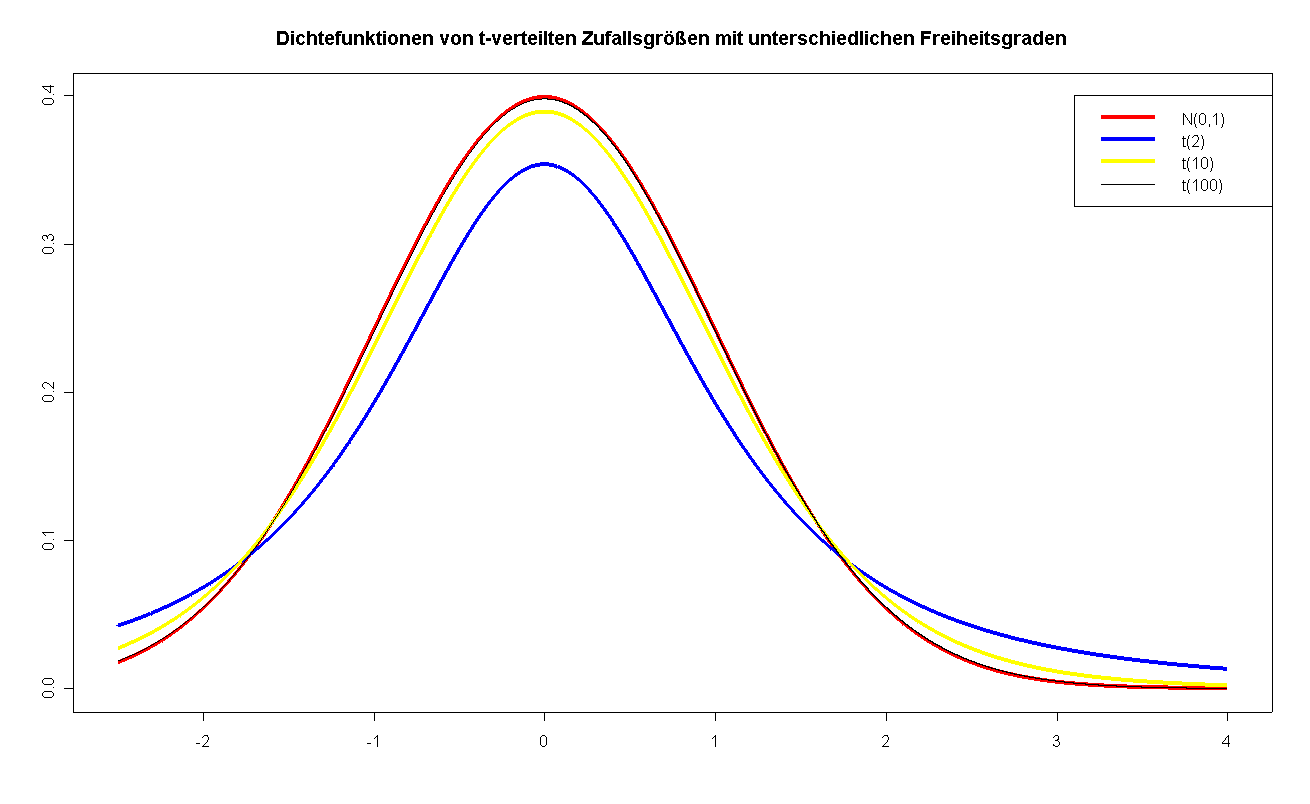
\includegraphics[scale=0.3]{figures/T-distribution.png}
\footnotesize{(Quelle: \url{https://de.wikipedia.org/wiki/Studentsche_t-Verteilung})}
\end{figure}

\noindent Die Grafik verdeutlicht die Annäherung der t-Verteilung mit zunehmenden Freiheitsgraden an die Standardnormalverteilung.\\

\noindent \framebox[\textwidth]{\texttt{R-Befehl für die t-Verteilung: > \_t()}\\ \mbox{} \hfill \href{https://www.rdocumentation.org/packages/stats/versions/3.6.2/topics/TDist}{Dokumentation}}

\subsubsection{F--Verteilung}\label{sec:fdistr}

\paragraph{Idee/Anwendung:} Auch für die F-Verteilung müssen wir ohne weitere Intuition auskommen. Sie wird wiederum für diverse theoretische Konzepte benutzt. 

\paragraph{Verteilung:}
\begin{itemize}
\item[] Notation: $X \sim F_{df_1,df_2}$
\end{itemize}

\noindent \dangersign Die F-Verteilung hat zwei Freiheitsgrade. Bitte denkt immer an beide (z.B. bei einem Overall-F-test für die Betakoeffizienten eines multiplen Regressionsmodells)!\\

\noindent \framebox[\textwidth]{\texttt{R-Befehl für die F-Verteilung: > \_f()}\\ \mbox{} \hfill \href{https://www.rdocumentation.org/packages/stats/versions/3.6.2/topics/FDist}{Dokumentation}}

\clearpage

\subsubsection{Aufgaben II}
\paragraph{1.Welche Aussagen zur stetigen Gleichverteilung sind richtig?}
\begin{itemize}
    \item[a)] Jede mögliche Ausprägung kommt mit einer Wahrscheinlichkeit von 0 vor. \hfill $\square$
    \item[b)] Der Unterschied zwischen der stetigen und diskreten Gleichverteilung ist, dass die\\ stetige Gleichverteilung unendlich verschiedene Werte annehmen kann. \hfill $\square$
    \item[c)] Die Dichtefunktion ist das Pendant zur Verteilungsfunktion.
    \item[d)] Die Dichtefunktion bei der stetigen Gleichverteilung ist eine monoton steigende Gerade. \hfill $\square$
    \item[e)] Die Dichtefunktion ($X \sim U(2,6)$) verläuft auf der Höhe 0,25. \hfill $\square$
\end{itemize}

\paragraph{2. Welche Aussagen zur Exponentialverteilung sind richtig?}
\begin{itemize}
    \item[a)] Die zukünftige Wartezeit ist abhängig von der davor schon verstrichenen Zeit. \hfill $\square$
    \item[b)] Bei der Exponential-, wie auch der geometrischen Verteilung geht es darum, wann das\\ gewünschte Ereignis zum ersten Mal auftritt. \hfill $\square$
    \item[c)] Die Exponentialverteilung ist nur für $X \geq 0$ definiert. \hfill $\square$
    \item[d)] Ein zentraler Begriff bei der Exponentialverteilung ist die Gedächtnislosigkeit. \hfill $\square$
\end{itemize}

\paragraph{3. Welche Aussagen zur Normalverteilung / Chi-Quadrat-Verteilung sind wahr?}
\begin{itemize}
    \item[a)] Die Dichtefunktion ist bei beiden symmetrisch um den Erwartungswert. \hfill $\square$
    \item[b)] Der Durchschnitt von i.i.d. normalverteilten Zufallsvariablen ist normalverteilt.\hfill $\square$ 
    \item[c)] Um die Dichtefunktion der Normalverteilung aufzustellen benötigt man nur $\sigma$ und $\mu$. \hfill $\square$
    \item[d)] Die Verteilungsfunktion der Normalverteilung hat bei $\mu$ ihr Maximum. \hfill $\square$
    \item[e)] Für die Chi-Quadrat-Verteilung werden die Quadrate von mehreren\\ standardnormalverteilten Zufallsvariablen gebildet und aufsummiert. \hfill $\square$
\end{itemize}

\paragraph{4. Welche Aussagen über die t-Verteilung sind richtig?}
\begin{itemize}
    \item[a)] Die t-Verteilung kann immer durch die Standardnormalverteilung approximiert werden. \hfill $\square$
    \item[b)] Je größer die Stichprobe, desto näher kommt sie der Standardnormalverteilung. \hfill $\square$
    \item[c)] Die Wahrscheinlichkeitsmasse an den Rändern ist bei der t-Verteilung geringer \\als bei der Standardnormalverteilung. \hfill $\square$
    \item[d)] Je weniger Freiheitsgrade, desto ähnlicher ist die t-Verteilung der Standard-\\normalverteilung. \hfill $\square$
\end{itemize}

\clearpage

\subsection{Wichtige Schlüsselbegriffe und "Konzepte" anhand der diskreten Gleichverteilung} \label{sec:concept}

\subsubsection{Parameter von Verteilungen}\label{sec:Param}

Mögliche Ergebnisse werden oft mit den Variablen $x_1,x_2,...,x_n$ bezeichnet. Für das Beispiel des Roulette-Spiels wären $x_1=0,x_2=1,...,x_{37}=36$. Die \textbf{Parameter} im Fall der diskreten Gleichverteilung werden oft als a und b definiert. Beim Roulettespiel gilt: $a = 0$ und $b = 36$, d.h. a und b sind sozusagen die Grenzen des Ergebnisraums.

\subsubsection{Träger einer Verteilung} \label{sec:Träger}
Der \textbf{Träger} der diskreten Gleichverteilung sind alle Ausprägungen $x_1,...,x_n$, also alle natürlichen Zahlen zwischen den (und einschließlich der) Grenzen a und b. Beim Roulette-Beispiel also alle Zahlen von $0,..,36$. 

\subsubsection{Verteilungsfunktion, Wahrscheinlichkeitsfunktion und Dichtefunktion} \label{sec:Functions}
In der Statistik I Vorlesung haben wir schon die empirische Verteilungsfunktion kennengelernt (z.B. als Treppenfunktion oder Polygonzug). Eine \textbf{Verteilungsfunktion} ist grob gesagt einfach nur eine Art Hilfestellung zur Beschreibung von diskreten/stetigen Wahrscheinlichkeitsverteilungen. Sie wird oftmals als Funktion $F$ definiert, die jedem Ergebnis $x_i$ einer Zufallsvariablen $X$ eine Wahrscheinlichkeit $P(X \leq x_i)$ zuordnet. Mathematisch ausgedrückt einfach nur:

\begin{equation*}
F: x \rightarrow P(X \leq x_i)
\end{equation*}

\noindent Sowohl die \textbf{Wahrscheinlichkeitsfunktion}\footnote{Die Wahrscheinlichkeitsfunktion wird häufig auch Dichte genannt und mit $f(x)$ notiert} für diskrete ZVs als auch die \textbf{Dichtefunktion} für stetige ZVS dienen als Beschreibung von Wahrscheinlichkeitsverteilungen. Sie beschreiben Wahrscheinlichkeiten für jedes mögliche Ergebnis $x_i$ eines Zufallsexperiments (mathematisch einfach $P(X=x_i)$). Oftmals wird sie aber einfach als $f(x)$ definiert. Liegt eine \textbf{stetige ZV} zugrunde, besitzt die Dichtefunktion folgende Eigenschaften:

\begin{enumerate}
    \item Die Funktion besitzt keinen negativen Wert: also $f(x)\geq 0$ für alle $x_i \in \mathbb{R}$
    \item Die Fläche unter der Funktion (berechnet als ihr Integral) ergibt 1 (analog diskrete ZV: Summe aller Einzelwahrscheinlichkeiten ergibt ebenfalls 1) -- mathematisch: $\int_{-\infty}^{\infty} f(x) dx = 1$
    \begin{itemize}
	\item[$\rightarrow$] Die Integralgrenzen können durch die Grenzen des Definitionsbereichs ersetzt werden.
	\end{itemize}
\end{enumerate}

\clearpage

\noindent Wichtige mathematische Zusammenhänge zwischen der Verteilungsfunktion, der Dichtefunktion und der Quantilsfunktion sind folgende:

\begin{enumerate}
    \item $f(x)= \frac{d}{dx} F(x)$, d.h. die Dichte ist also einfach die Ableitung der Verteilungsfunktion.
    \item $F(x)= \int_{-\infty}^{x} f(t)dt$, d.h. die Verteilungsfunktion ist die Fläche unter der Dichte (also das Integral der Dichte).
    \item $Q(x)= F^{-1}(x)$, d.h. die Quantilsfunktion ist die Umkehrfunktion der Verteilungsfunktion. (Rückblick Statistik I: Quantile sind einfach nur bestimmte Schwellenwerte, d.h. ein bestimmter Anteil der Werte ist kleiner oder gleich dem Quantil, der Rest ist größer -- Beispiel: Median).
    \item $F(x) = Q^{-1}(x)$, d.h. die Verteilungsfunktion ist die Umkehrfunktion der Quantilsfunktion.
\end{enumerate}

\noindent Aber zurück zum Beispiel der diskreten Gleichverteilung unseres Roulette--Spiels:\\

\paragraph{Verteilungsfunktion:}
Allgemein ergibt sich für eine diskrete Gleichverteilung auf den ganzen Zahlen 
$\left\{a,a+1,a+2,\ldots, b-1, b\right\}$ für die Verteilungsfunktion:
\begin{equation*}
    F(x)=\begin{cases}
			0, & \text{x < a}\\
            \frac{\floor*{x}-a+1}{b-a+1}, & \text{$x \in [a,b]$}\\
            1, & \text{x > b}
		 \end{cases}
\end{equation*}

\noindent $\floor*{x}$ bedeutet, dass wir x abrunden, d.h. $\floor{3.7} = 3$. Speziell für das Beispiel Roulette: Will man z.B. wissen wie wahrscheinlich eine Zahl kleiner als 3.5 ist berechnet man:

\begin{equation*}
    F(3.5) = \frac{\floor*{3.5}-0+1}{36-0+1} = \frac{4}{37}
\end{equation*}


\paragraph{Wahrscheinlichkeitsfunktion:}
Die Wahrscheinlichkeitsfunktion sieht folgendermaßen aus:

\begin{equation*}
    f(x)=\begin{cases}
			\frac{1}{37}, & \text{$x \in \{0,1,2,..,36\}$}\\
            0, & \text{sonst}
		 \end{cases}
\end{equation*}


\subsubsection{Erwartungswert und Varianz} \label{sec:Expec}
Der \textbf{Erwartungswert} der diskreten Gleichverteilung ist definiert als $E(X) = \frac{a+b}{2}$ und die Varianz ist definiert als $Var(X) = \frac{(b-a+1)^2-1}{12}$. Vorsicht: Dies sind etwas allgemeinere Formeln als der Spezialfall in der Formelsammlung, im Prinzip stellt es aber das Gleiche dar.

\clearpage

\subsubsection{Aufgaben III}
\paragraph{1. Welche Aussagen sind richtig?}
\begin{itemize}
    \item[a)] Der Träger der diskreten Gleichverteilung eines Münzwurfs sind Kopf und Zahl. \hfill $\square$
    \item[b)] Eine Verteilungsfunktion geht immer von -1 bis 1. \hfill $\square$
    \item[c)] Der Wert einer Verteilungsfunktion an der Stelle $x=5$ ist $P(X\leq 5)$.\hfill $\square$
    \item[d)] Die Werte der Verteilungsfunktion sind die kumulierten Wahrscheinlichkeiten. \hfill $\square$
    \item[e)] Die Wahrscheinlichkeitsfunktion ist bei diskreten Zufallsvariablen das Gleiche wie \\die Verteilungsfunktion bei stetigen Zufallsvariablen. \hfill $\square$
\end{itemize}

\paragraph{2. Welche Aussagen sind richtig?}
\begin{itemize}
    \item[a)] Die Verteilungsfunktion ist monoton steigend. \hfill $\square$
    \item[b)] Die Verteilungsfunktionen von stetigen Zufallsvariablen sind Treppenfunktionen \\im Gegensatz zu den diskreten Zufallsvariablen. \hfill $\square$
    \item[c)] Eine Eigenschaft der diskreten Verteilungsfunktion ist, dass die Fläche unterhalb \\der Funktion immer 1 ergibt. \hfill $\square$
    \item[d)] Die Summe aller Einzelwahrscheinlichkeiten bei einer stetigen Zufallsvariable ergibt 1. \hfill $\square$
    \item[e)] Eine Eigenschaft der Dichtefunktion einer stetigen ZV ist, dass die Funktionswerte\\immer größer gleich 0 sind. \hfill $\square$
\end{itemize}

\paragraph{3. Welche Aussagen sind richtig?}
\begin{itemize}
    \item[a)] Um die Verteilungsfunktion zu erhalten, leitet man die Dichtefunktion ab .\hfill $\square$
    \item[b)] Die Fläche unter der Dichtefunktion ist die Quantilsfunktion. \hfill $\square$
    \item[c)] Die Quantilsfunktion ist die Umkehrfunktion der Verteilungsfunktion. \hfill $\square$
    \item[d)] Die Ableitung der Verteilungsfunktion ist die Dichte. \hfill $\square$
\end{itemize}


\clearpage

%%%%%%%%%%%%%%%%%%%%%%%%%%%%%%%%%%%%%
%%%%%%%%%%  KAPITEL 15
%%%%%%%%%%%%%%%%%%%%%%%%%%%%%%%%%%%%%

\section{Grenzwertsätze und Approximationen von Verteilungen} \label{sec:GWSapprox}

Dieses Kapitel der Vorlesung beschreibt Grundbegriffe über das Verhalten von Folgen von Zufallsvariablen, wenn $n$ gegen unendlich strebt. Die "normale" mathematische Folge sollte schon aus der Vorlesung "Mathematik für Wirtschaftswissenschaftler" bekannt sein. Diese Idee wird nun durch das Hinzunehmen von Zufallsvariablen erweitert. Für eine Auffrischung der Theorie von Folgen und Reihen siehe: 
\href{https://www.statistik.uni-muenchen.de/formulare/skripte_u_aehnliches/mathehandrechnung_schneider.pdf}{Handreichung von Frau Dr. Dr. Schneider}

\subsection{Grenzwertsätze}\label{sec:GWS}
\subsubsection{Gesetz der großen Zahlen}\label{sec:LLN}

Das Gesetz der großen Zahlen besagt, dass sich beobachtete relative Häufigkeiten mit zunehmendem $n$ immer näher an die theoretischen Wahrscheinlichkeiten annähern. Genau dann konvergiert die durchschnittliche mittlere Abweichung zwischen den Zufallsvariablen $X_i$ und ihrem Erwartungswert $E(X_i)$ gegen Null. Die Gesetzmäßigkeit lässt sich dadurch erklären, dass der Einfluss von Ausreißern mit zunehmendem Stichprobenumfang des Experiments abnimmt. Man kann sich dies z.B. anhand des einfachen Münzwurfs klarmachen: Wirft man eine Münze 10 mal, wird sich nur in seltenen Fällen genau eine relative Häufigkeit von $1/2$ für Kopf oder Zahl ergeben. Wirft man sie dagegen 1000 mal, wird der Wert sehr nahe an $1/2$ liegen. 


\subsubsection{Zentraler Grenzwertsatz (ZGS)}\label{sec:ZGS}
Der zentrale Grenzwertsatz gehört zu den wichtigsten Aussagen der Wahrscheinlichkeitstheorie. Er gibt eine Charakterisierung der Normalverteilung als Grenzverteilung von Überlagerungen einer Vielzahl unabhängiger zufälliger Einzeleffekte. Der ZGS besagt, dass sich der Mittelwert einer jeden beliebigen Verteilung von iid Zufallsvariablen mit zunehmenden Stichprobenumfang der Normalverteilung annähern wird. Wegen des zentralen Grenzwertsatzes können wir Hypothesentests durchführen, auch wenn die Grundgesamtheit keiner Normalverteilung unterliegt, vorausgesetzt, dass die Stichprobe ausreichend groß ist.\\

\noindent \dangersign Vorsicht: Oftmals wird angenommen, dass der zentrale Grenzwertsatz sagt, dass eine Stichprobe ab einer gewissen Größe automatisch normalverteilt sein wird. Dies stimmt aber nicht!


\subsection{Approximationen}\label{sec:Approx}
Wir können unter bestimmten Voraussetzungen Verteilungen durch andere Verteilungen approximieren. Doch warum und wann sind Approximationen sinnvoll?

\begin{itemize}
    \item Bei Rechenintensiven Tasks.
    \item Bei  diskreten Verteilungen: Addition vieler Einzelwahrscheinlichkeiten wird vermieden.
    \item Bei Approximation durch Normalverteilung: Standardisierung möglich.
\end{itemize}

\noindent Insgesamt haben wir vier Approximationen kennengelernt, die nachfolgend nochmal -- überwiegend bezüglich ihrer Intuition -- besprochen werden.\\

\noindent \dangersign Sehr wichtig: Immer die Annahmen für die Approximation prüfen.

\subsubsection{Approximation der Binomial- durch die Normalverteilung}\label{sec:BinN}

\paragraph{Voraussetzung:} $np(1-p) \geq 9$
\paragraph{Approximation:} $B(n,p) \rightarrow \mathcal{N}(np,np(1-p))$
\paragraph{Intuition:} Bei erfüllter Voraussetzung ist die Wahrscheinlichkeitsfunktion der Binomialverteilung (annähernd) symmetrisch und sieht der Dichte der Normalverteilung sehr ähnlich. In diesem Fall ist die Approximation zulässig. Um euch davon zu überzeugen, wie die Wahrscheinlichkeitsfunktion der Binomialverteilung für verschiedene $n$ und $p$ aussieht könnt ihr auf der Seite \url{https://matheguru.com/stochastik/binomialverteilung.html} das Tool "Interaktive Binomialverteilung" nutzen und verschiedene Kombinationen für $n$ und $p$ ausprobieren. Ihr könnt z.B. Werte, die die Voraussetzung nicht erfüllen, mit Werten, die die Voraussetzung erfüllen, vergleichen. Beachtet dabei, dass ihr "PDF" anklickt (und nicht "CDF").
\paragraph{Bemerkung 1:} Auch bei z.B. $n=10$ und $p=0.5$ ist die Wahrscheinlichkeitsfunktion symmetrisch und sieht der Normalverteilung ähnlich. Wir dürfen trotzdem nicht approximieren (vgl. $10\cdot0.5\cdot0.5=2.5<9$). Der Grund dafür, dass wir hier noch nicht approximieren dürfen ist, dass wir eine diskrete Verteilung (Binomialverteilung) durch eine stetige Verteilung (Normalverteilung) approximieren. Die Schritte in der Wahrscheinlichkeitsfunktion sind einfach noch zu groß, um durch eine stetige Verteilung approximiert werden zu dürfen.
\paragraph{Bermerkung 2:} Außerdem gilt nach dieser Approximation, dass die ZV $\hat{p}=\frac{1}{n} \sum X_i$ auch normalverteilt ist: $\hat{p} \sim \mathcal{N}\Big(p,\frac{p(1-p)}{n}\Big)$

\subsubsection{Approximation der Binomial- durch die Poissonverteilung}\label{sec:BinPo}

\paragraph{Voraussetzung:} Großes $n$ und kleines $p$.
\paragraph{Approximation:} $B(n,p) \rightarrow Po(np)$
\paragraph{Intuition:} Da wir sowohl die Binomial- als auch die Poissonverteilung durch die Normalverteilung approximieren können (wenn die entsprechenden Voraussetzungen erfüllt sind), ist diese Approximation dann einfach nur logisch (vgl. dazu $B(0,05;200)$ und $Po(10)$). \textit{Aber was ist, wenn die jeweiligen Voraussetzungen nicht erfüllt sind?} In diesem Fall schauen wir uns einfach wieder die Binomialverteilung für ein großes $n$ und ein kleines $p$ in dem Tool "Interaktive Binomialverteilung" an: 
	 Die Binomialverteilung ist rechtsschief/linkssteil (für kleine $p$). Dann ist $np$ auch so klein, dass die Poissonverteilung rechtsschief/linkssteil ist (vgl. Poissonverteilung mit $\lambda=1$, z.B. als Approximation für die Binomialverteilung mit $p=0,01$ und $n=100$).


\subsubsection{Approximation der Poisson- durch die Normalverteilung}\label{sec:PoN}
\paragraph{Voraussetzung:} $\lambda \geq 10$
\paragraph{Approximation:} $Po(\lambda) \rightarrow \mathcal{N}(\lambda,\lambda)$\footnote{Zur Erinnerung: Für $Po(\lambda)$ gilt $\E[X]=Var[X]=\lambda$, d.h. man übernimmt Erwartungswert und Varianz der Poissonverteilung einfach als Parameter für die Normalverteilung.}
\paragraph{Intuition:} Auch hier schauen wir uns einfach die Wahrscheinlichkeitsfunktion der Poissonverteilung an und sehen, dass diese mit steigendem $\lambda$ \textit{immer symmetrischer} wird. Und wenn letztere annähernd symmetrisch ist (ab $\lambda = 10$), können wir durch die symmetrische Normalverteilung approximieren. Außerdem ist hierbei wichtig, dass die Normalverteilung "weit genug" auf dem positiven Teil der x-Achse liegt und negative Werte nur mit einer sehr, sehr geringen Wahrscheinlichkeit vorkommen, da die Poissonverteilung ja Anzahlen modelliert, die immer nicht-negativ sind. Das ist wiederum erfüllt, wenn die Normalverteilung um $\lambda=\mu \geq 10$ zentriert ist.\\

\noindent Zur Veranschaulichung könnt ihr ein ähnliches Tool wie für die Binomialverteilung nutzen. Ihr findet es unter \url{https://matheguru.com/stochastik/poisson-verteilung.html}.

\subsubsection{Approximation der hypergeometrischen durch die Binomialverteilung}\label{sec:HypBin}

\paragraph{Voraussetzungen:} \begin{enumerate}
\item $n \leq 0,1\cdot M$
\item $n \leq 0,1\cdot (N-M)$
\end{enumerate}
\paragraph{Approximation:} $H(n,M,N) \rightarrow B(n, \frac{M}{N})$
\paragraph{Intuition:} Hinter dieser Approximation steckt, dass jedes Ziehen (insgesamt $n$--mal) mit der hypergeometrischen Verteilung ein Bernoulli-Experiment ist, ob das gewünschte Merkmal gezogen wird oder nicht. Beim ersten Ziehen ist noch sehr offensichtlich, dass die Wahrscheinlichkeit, das gewünschte Merkmal zu ziehen, $p=\frac{M}{N}$ ist. Nach jedem Zug reduzieren sich aber $N$ bzw. $N$ und $M$, d.h. $p$ im einfachen Bernoulli-Experiment verändert sich. Bei erfüllten Faustregeln hingegen ist die Anzahl der Züge im Vergleich zur Anzahl der Objekte mit dem gewünschten Merkmal ($M$) bzw. ohne das gewünschte Merkmal ($N-M$) so gering, dass angenommen werden kann, dass sich $p$ nicht ändert. D.h. wir nehmen $p=\frac{M}{N}$ als konstant an. Dann sind die $n$ Züge unabhängige Bernoulli-Experimente und daher ist die Approximation durch die Binomialverteilung zulässig.

\clearpage

\subsection{Aufgaben}
\paragraph{1.Welche Aussagen bzgl.den Grenzwertsätzen ist wahr?}
\begin{itemize}
    \item[a)] Je größer der Stichprobenumfang, desto größer wird der Einfluss von Ausreißern. \hfill $\square$
    \item[b)] Mit zunehmendem Stichprobenumfang nähert sich die beobachtete relative Häufigkeit\\ der theoretischen Wahrscheinlichkeit an. \hfill $\square$
    \item[c)] Egal welche Verteilung vorliegt, nähert sich der Mittelwert von i.i.d. Zufallsvariablen\\ bei zunehmenden Stichprobenumfang der Normalverteilung an. \hfill $\square$
\end{itemize}

\paragraph{2. Welche Aussagen bzgl. Approximationen sind richtig?}
\begin{itemize}
    \item[a)] Die hypergeom. Verteilung kann durch die Normalverteilung approximiert werden. \hfill $\square$
    \item[b)] Bei der Approximation der Poissonverteilung durch die Normalverteilung wird das $\lambda$\\ für das $\mu$ und das $\sigma$ einfach übernommen. \hfill $\square$
    \item[c)] Die Poissonverteilung darf immer durch die Normalverteilung approximiert werden. \hfill $\square$
    \item[d)] Die hypergeometrische Verteilung H(9,120,40) darf durch die Binomialverteilung \\approximiert werden. \hfill $\square$
\end{itemize}


\clearpage

%%%%%%%%%%%%%%%%%%%%%%%%%%%%%%%%%%%%%
%%%%%%%%%%  KAPITEL 16
%%%%%%%%%%%%%%%%%%%%%%%%%%%%%%%%%%%%%

\section{Schätzen}\label{chap:schaetzen}

\subsection{Die Maximum Likelihood Schätzung}\label{sec:ML}

Die ML Schätzung ist ein Prinzip für die Konstruktion von Parameterschätzern bei gegebener Verteilung einer Zufallsvariable.\\

\paragraph{Idee:} Wähle die Schätzwerte für die wahren Parameter der Grundgesamtheit so, dass unter diesen die beobachtete Stichprobe am wahrscheinlichsten sind (dies erklärt auch den Namen der Methode). Die ML-Methode beinhaltet 5 Schritte:

\begin{enumerate}
    \item Liegt eine iid-Stichprobe vor?
    \item Bestimme die Dichte für die einzelnen Beobachtungen.
    \item Stelle die Likelihoodfunktion auf.
    \item Stelle die log-Likelihoodfunktion auf.
    \item Maximiere die log-Likelihood (Ableitung und 0 setzen) und prüfe die Bedingung 2. Ordnung (Maximim oder Minimum?).
\end{enumerate}

\noindent Beispiele der ML-Schätzung für Normalverteilung, Binomialverteilung, Poissonverteilung und Exponentialverteilung:\\
\url{https://mars.wiwi.hu-berlin.de/mediawiki/mmstat3/index.php/Maximum-Likelihood-Methode}

\clearpage

\subsection{Konfidenzintervalle (KI)}\label{sec:KI}

\paragraph{Wozu braucht man eigentlich Konfidenzintervalle?} In der induktiven Statistik wird mit Hilfe einer Stichprobe versucht, allg. Aussagen über die Grundgesamtheit zu machen. Mit der ML-Schätzung haben wir dafür schon eine Methode kennengelernt um Punktschätzer zu "generieren". Die erhobenen Daten einer Stichprobe werden dann in einem Punktschätzer zusammengefasst (z.B. Mittelwert oder Varianz), um damit auf die wahren Werte in der Grundgesamtheit zu schließen.\\

\noindent \dangersign Probleme:

\begin{itemize}
    \item Wie präzise ist diese Punktschätzung eigentlich?
    \item In welchem Bereich liegt der wahre Mittelwert der Grundgesamtheit höchstwahrscheinlich?
    \item Ist es möglich, dass in Wirklichkeit im Mittel doch ein anderer Wert herauskommt, aber wir in dieser Stichprobe einfach nur Pech hatten?
\end{itemize}

\noindent $\Rightarrow$ Diese Fragen kann ein Punktschätzer nicht beantworten – aber ein Intervallschätzer kann das!

\paragraph{Doch was ist ein Konfidenzintervall genau?} Die folgende Unterscheidung ist sehr wichtig für das Verständnis von Konfidenzintervallen:

\begin{itemize}
    \item Mit einer Stichprobe schätzen wir einen Parameter, z.B $\hat{\mu}$.
    \item Das wahre $\mu$ in der Grundgesamtheit ist zwar in der Nähe von $\hat{\mu}$, aber quasi nie genau gleich.
\end{itemize}

\noindent Den wahren Parameter $\mu$ werden wir also nie exakt bestimmen können, dennoch können wir versuchen einen Bereich zu bestimmen in dem er ziemlich sicher liegt -- und genau das ist die Idee von Konfidenzintervallen.

\paragraph{Definition KI (ohne Formel):} Ein 95\%-KI ist ein Intervall [a,b], das, wenn es sehr häufig mit neuen Stichproben berechnet wird, den wahren Parameter, z.B. $\mu$, mit einer Wahrscheinlichkeit von 95\% auch überdeckt. $\Rightarrow$ ein einzelnes 95\%-KI ist mit 95\%-iger Wahrscheinlichkeit eines von denen, das den wahren Parameter ($\mu$) beinhaltet.

\paragraph{Und wie schätzt man ein Konfidenzintervall?} Zentrale Prinzip für alle Konfidenzintervalle:

\begin{enumerate}
    \item Punktschätzer für einen Parameter berechnen, z.B. für den Anteilswert $p$ einer Bernoulli-/Binomialverteilung.
    \item Um den Punktschätzer bildet man ein (meist) symmetrisches Intervall, das abhängig von der Varianz in der Stichprobe und gewünschtem Konfidenzniveaus $1-\alpha$ enger oder breiter ist.
\end{enumerate}

\noindent \framebox[\textwidth]{\texttt{R-Befehl für Konfidenzintervalle: > ci()}\\ \mbox{} \hfill \href{https://www.rdocumentation.org/packages/gmodels/versions/2.18.1/topics/ci}{Dokumentation}}

\noindent \dangersign Die R-Funktion ist \textbf{nicht} Teil von \texttt{base-R} sondern Teil des Paketes \texttt{gmodels}. Dieses muss zunächst installiert (\texttt{install.packages("gmodels")}) und anschließend importiert werden (\texttt{library(gmodels)}).

\clearpage

\subsection{Aufgaben}
\paragraph{Welche Aussagen ist bzgl. Punkt- \& Intervallschätzer sind richtig?}
\begin{itemize}
    \item[a)] Punktschätzer sind immer richtig und wahrheitsgetreu. \hfill $\square$
    \item[b)] Ein Konfidenzintervall gibt den Bereich vor, in dem der wahre Parameter immer \\zu finden ist. \hfill $\square$
    \item[c)] Man kann die Länge eines Intervalls variieren, je nach dem mit welcher\\ Wahrscheinlichkeit der wahre Parameter durch das Intervall überdeckt werden soll. \hfill $\square$
    \item[d)] Die Länge eines Intervalls hängt von $\alpha$, $\sigma^2$, der Verteilung und dem Stichproben-\\umfang ab. \hfill $\square$
    \item[e)] Ein 99$\%$-KI besagt, dass zu 99$\%$ mein Schätzer richtig ist. \hfill $\square$
\end{itemize}


\clearpage

%%%%%%%%%%%%%%%%%%%%%%%%%%%%%%%%%%%%%
%%%%%%%%%%  KAPITEL 17
%%%%%%%%%%%%%%%%%%%%%%%%%%%%%%%%%%%%%

\section{Testtheorie}\label{sec:Tests}

\subsection{Der p-Wert}\label{sec:pWert}

Der p-Wert gibt die Wahrscheinlichkeit an, dass die Teststatistik, unter der Annahme, dass $H_0$ wahr ist, den beobachteten/realisierten Wert $t$ oder einen noch extremeren Wert annimmt. Noch extremer heißt in diesem Fall, dass man sich davon wegbewegt, $H_0$ anzunehmen. Um das zu verdeutlichen, müssen wir uns erstmal vor Augen halten, wo genau diese Wahrscheinlichkeit herkommt: \\

\noindent Wir wissen, dass die Teststatistik $T(\textbf{X})$ unter $H_0$ eine bestimmte Verteilung hat (Merke: $T(\textbf{X})$ ist eine ZV). Von dieser Verteilung kommen ja dann auch die Quantile, die wir als kritische Werte heranziehen, um die Testentscheidung mittels der Teststatistik zu treffen. Was genau das mit dem p-Wert zu tun hat, gehen wir jetzt am Beispiel eines einseitigen und eines zweiseitigen t-Tests durch.

\subsubsection{Der p-Wert beim einseitigen t-Test}\label{sec:pWert1}

Der einseitige t-Test wird genutzt, um zu testen, ob der Erwartungswert einer normalverteilten ZV größer (kleiner) als ein unter $H_0$ angenommener Wert $\mu_0$ ist, wenn die Varianz $\sigma^2$ unbekannt ist und geschätzt werden muss.  Man kann die Hypothese (je nachdem, was man zeigen möchte) für beide Richtungen aufstellen. Wir zeigen es an dem Beispiel, dass wir testen wollen, ob der Erwartungswert signifikant kleiner als ein $\mu_0$ ist. D.h. die Hypothesen lauten:
$$H_0: \mu \geq \mu_0 \qquad \mbox{vs.} \qquad H_1: \mu < \mu_0$$

\noindent Die Teststatistik und ihre Verteilung sind dann unter der $H_0$--Hypothese:
$$T(\textbf{X})=\sqrt{n}\cdot\frac{\overline{X}-\mu_0}{S_x} \simtext{$H_0$} t_{n-1}$$

\noindent Mit den vorliegenden Daten berechnet man nun eine Realisation $t$ der Zufallsvariable T(\textbf{X}). Dann wird $H_0$ abgelehnt, wenn $t \in (-\infty, -t_{n-1,1-\alpha})$. Je kleiner die Realisation $t$ von T(\textbf{X}) also ist, desto eher lehnen wir $H_0$ ab bzw. desto weiter entfernen wir uns davon, $H_0$ anzunehmen. Die Wahrscheinlichkeit, dass man dann eine genauso kleine oder noch kleinere Teststatistik (im Vergleich zur Realisation $t$) erhält, wenn man die unter $H_0$ angenommene Verteilung ($t_{n-1}$) zugrunde legt, ist dann der p-Wert, also:
$$p-Wert=P(T \leq t),$$
wobei T ($\sim t_{n-1}$) wieder die ZV ist und $t$ die Realisation. Ist diese Wahrscheinlichkeit kleiner als das Signifikanzniveau $\alpha$, dann ist es sehr unwahrscheinlich, dass die Realisation $t$ von der ZV $T(\textbf{X})$ "unterboten" wird, wenn denn die Verteilungsannahme aus $H_0$ stimmt. Aber wenn es eben so unwahrscheinlich ist, dass $t$ von der ZV $T(\textbf{X})$ unterboten wird, muss $t$ selbst (unter der Verteilung in $H_0$) ein Ausreißer, also ein seltenes Ereignis sein.\\
D.h. wir hätten mit unseren Daten zufällig ein seltenes Ereignis getroffen. Wir wollen aber nicht glauben, dass wir ausgerechnet ein seltenes Ereignis gefunden haben und verwerfen deshalb die unter $H_0$ angenommene Verteilung und somit die $H_0$--Hypothese.

\paragraph{Merke:} $p-Wert=P(T \leq t) < \alpha$ $\Rightarrow$ $H_0$ verwerfen!\\

\noindent \dangersign Für die Hypothesen: 
$$H_0: \mu \leq \mu_0 \qquad \mbox{vs.} \qquad H_1: \mu > \mu_0$$

\noindent ist der p-Wert entsprechend:
$$p-Wert=P(T \geq t)=1-P(T < t)$$

\noindent da wir ja dann den Ablehnbereich $(t_{n-1,1-\alpha}, + \infty)$ haben.

\subsubsection{Der p-Wert beim zweiseitigen t-Test}\label{sec:pWert2}

Hier werden folgende Hypothesen gegeneinander getestet:
$$H_0: \mu = \mu_0 \qquad \mbox{vs.} \qquad H_1: \mu \neq \mu_0$$

\noindent Die Teststatistik ist wiederum:
$$T(\textbf{X})=\sqrt{n}\cdot\frac{\overline{X}-\mu_0}{S_x} \simtext{$H_0$} t_{n-1}$$

\noindent und der Ablehnbereich ist: $(-\infty, -t_{n-1,1-\frac{\alpha}{2}}) \cup (t_{n-1,1-\frac{\alpha}{2}}, +\infty)$.

\noindent D.h. dann, dass wir uns sowohl für Teststatistiken, die größer als $t_{n-1,1-\frac{\alpha}{2}}$ sind, immer mehr vom Annahmebereich entfernen als auch für Teststatistiken, die kleiner als $-t_{n-1,1-\frac{\alpha}{2}}$ sind. Für den p-Wert bedeutet das, dass wir beide Richtungen berücksichtigen müssen (was wir mit Hilfe des Betrags der Teststatistik machen, wobei wir die Symmetrie der t-Verteilung ausnutzen):
\begin{align*} 
p-Wert &= P(|T| \geq |t|)  \\
	&=	P(T \leq -|t|) + P(T \geq |t|)			\\
	&=	2 \cdot P(T \geq |t|)			\\
	&=	2 \cdot (1-P(T < |t|))			\\
	&=	2 \cdot (1-F(|t|)),		
\end{align*} 

\noindent wobei $F(\cdot)$ die Verteilungsfunktion der entsprechenden Verteilung ist -- hier also der t-Verteilung mit $n-1$ Freiheitsgraden.


\subsection{Hypothesentests}\label{sec:HypTests}

In der Vorlesung haben wir eine Reihe von Hypothesentests kennengelernt. Auf die wichtigsten wird hier noch einmal intuitiv eingegangen. Bevor wir auf die verschiedenen Tests eingehen eine kleine Bemerkung zu einfachen bzw. doppelten und einseitigen bzw. zweiseitigen Tests:
Ein einfacher Test (im Vergleich zu einem doppelten Test) betrachtet eine einzige Stichprobe. Der einfache Test kann aber sowohl einseitig ($H_0:$ $\mu \geq \mu_0$ gg. $H_1:$ $\mu < \mu_0$ bzw. umgekehrt) als auch zweiseitig ($H_0:$ $\mu = \mu_0$ gg. $H_1:$ $\mu \neq \mu_0$) formuliert werden. Ein doppelter Test hingegen betrachtet zwei Stichproben -- auch dieser kann sowohl ein- als auch zweiseitig formuliert werden.

\subsubsection{Einfacher Gauss-Test}\label{sec:Gausstest1}
Test des Erwartungswerts $\mu_x$ einer (per Annahme) normalverteilten ZV $X$ ($\sim \mathcal{N}(\mu_x, \sigma_x^2)$). Die \textbf{Varianz} $\sigma_x^2$ ist dabei \textbf{bekannt}. \\

\noindent \framebox[\textwidth]{\texttt{R-Befehl für den einfachen Gauss-Test: > gausstest(data\$x)}\\ \mbox{} \hfill \href{https://www.rdocumentation.org/packages/compositions/versions/2.0-0/topics/gausstest}{Dokumentation}}

\noindent \dangersign Die R-Funktion ist \textbf{nicht} Teil von \texttt{base-R} sondern Teil des Paketes \texttt{compositions}. Dieses muss zunächst installiert (\texttt{install.packages("compositions")}) und anschließend importiert werden (\texttt{library(compositions)}).

\subsubsection{Einfacher t-Test}\label{sec:tTest1}
Test des Erwartungswerts $\mu_x$ einer (per Annahme) normalverteilten ZV $X$ ($\sim \mathcal{N}(\mu_x, \sigma_x^2)$). Die \textbf{Varianz} $\sigma_x^2$ ist dabei \textbf{unbekannt} und muss aus der Stichprobe mittels der der Stichprobenvarianz $S^2$ geschätzt werden.\\

\noindent \framebox[\textwidth]{\texttt{R-Befehl für den einfachen t-Test: > t.test(data\$x)}\\ \mbox{} \hfill \href{https://www.rdocumentation.org/packages/stats/versions/3.6.2/topics/t.test}{Dokumentation}}

\subsubsection{Approximativer Einfacher Binomialtest}\label{sec:bintest1}
Test der Erfolgswahrscheinlichkeit $p$ einer (per Annahme) bernoulliverteilten ZV $X$ ($\sim B(1, p)$). Die Teststatistik ist approximativ standardnormalverteilt. \\

\noindent \framebox[\textwidth]{\texttt{R-Befehl \textbf{exakter} Binomialtest: > binom.test(data\$x)}\\ \mbox{} \hfill \href{https://www.rdocumentation.org/packages/stats/versions/3.6.2/topics/binom.test}{Dokumentation}}

\noindent \dangersign Dieser Befehl führt den \textbf{exakten} Binomialtest durch, der approximative kann mit der \texttt{gausstest}-Funktion durchgeführt werden.

\subsubsection{Chi-Quadrat-Anpassungstest}\label{sec:chitest1}
Test der unter $H_0$ erwarteten und tatsächlich Beobachteten absoluten Häufigkeiten von verschiedenen Ausprägungen einer ZV. Dadurch kann man testen, ob die Verteilung, von der die Stichprobe stammt, ungleich einer unter $H_0$ angenommenen Verteilung ist.

\subsubsection{F-Test}\label{sec:ftest}
Testet das Verhältnis (Größer/kleiner bzw. Gleichheit/Ungleichheit) der Varianzen zweier unabhängiger normalverteiler ZV. Die Teststatistik ist der Quotient der Stichprobenvarianzen und F-verteilt.\\

\noindent \dangersign Die F--Verteilung hat \textbf{zwei Freiheitsgrade}. Denkt immer an beide (z.B. auch bei der F-Statistik eines multiplen Regressionsmodells).\\

\noindent \framebox[\textwidth]{\texttt{R-Befehl für den F-Test: > var.test(data\$x, data\$y)}\\ \mbox{} \hfill \href{https://www.rdocumentation.org/packages/stats/versions/3.6.2/topics/var.test}{Dokumentation}}

\subsubsection{Doppelter Gauss-Test}\label{sec:Gausstest2}
Testet das Verhältnis (Größer/Kleiner bzw. Gleichheit/Ungleichheit) der Erwartungswerte zweier unabhängiger normalverteiler ZVs (X und Y). Die \textbf{Varianzen} $\sigma_x^2$ und $\sigma_y^2$ sind dabei \textbf{bekannt}.\\

\noindent \framebox[\textwidth]{\texttt{R-Befehl für den doppelten Gauss-Test: > gausstest(data\$x, data\$y)}\\ \mbox{} \hfill \href{https://www.rdocumentation.org/packages/compositions/versions/2.0-0/topics/gausstest}{Dokumentation}}

\noindent \dangersign Die R-Funktion ist \textbf{nicht} Teil von \texttt{base-R} sondern Teil des Paketes \texttt{compositions}. Dieses muss zunächst installiert (\texttt{install.packages("compositions")}) und anschließend importiert werden (\texttt{library(compositions)}). 

\subsubsection{Doppelter t-Test}\label{sec:tTest2}
Testet das Verhältnis (Größer/Kleiner bzw. Gleichheit/Ungleichheit) der Erwartungswerte zweier unabhängiger normalverteiler ZVs (X und Y). Die \textbf{Varianzen} $\sigma_x^2$ und $\sigma_y^2$ sind dabei \textbf{unbekannt} und müssen aus der Stichprobe mittels der der Stichprobenvarianz $S^2$ geschätzt werden. Hier wird zusätzlich angenommen, dass die zugrundeliegenden Verteilungen \textbf{beider ZVs dieselbe Varianz} haben ($\sigma_x^2 =\sigma_y^2$). \\

\noindent \framebox[\textwidth]{\texttt{R-Befehl doppelter t-Test: > t.test(data\$x,data\$y,var.equal=TRUE)}\\ \mbox{} \hfill \href{https://www.rdocumentation.org/packages/stats/versions/3.6.2/topics/t.test}{Dokumentation}}

\subsubsection{Welch-Test}\label{sec:Welch}
Testet das Verhältnis (Größer/Kleiner bzw. Gleichheit/Ungleichheit) der Erwartungswerte zweier unabhängiger normalverteiler ZV (X und Y). Die \textbf{Varianzen} $\sigma_x^2$ und $\sigma_y^2$ sind dabei \textbf{unbekannt} und müssen aus der Stichprobe mittels der der Stichprobenvarianzen $S_x^2$ und $S_y^2$ geschätzt werden. Hier wird zusätzlich angenommen, dass die zugrundeliegenden Verteilungen \textbf{beider ZVs ungleiche Varianzen} haben ($\sigma_x^2 \neq \sigma_y^2$). \\

\noindent \framebox[\textwidth]{\texttt{R-Befehl Welch-Test: > t.test(data\$x, data\$y, var.equal = FALSE)}\\ \mbox{} \hfill \href{https://www.rdocumentation.org/packages/stats/versions/3.6.2/topics/t.test}{Dokumentation}}

\subsubsection{Paired t-Test}\label{sec:paired}
Testet das Verhältnis (Größer/Kleiner bzw. Gleichheit/Ungleichheit) der Erwartungswerte zweier \textbf{abhängiger} normalverteiler ZV ($X$ und $Y$). Diese Abhängigkeit kann dadurch entstehen, dass man an denselben Untersuchungseinheiten dasselbe Merkmal zu verschiedenen Zeitpunkten misst.\\

\noindent \framebox[\textwidth]{\texttt{R-Befehl paired t-Test: > t.test(data\$x, data\$y, paired = TRUE)}\\ \mbox{} \hfill \href{https://www.rdocumentation.org/packages/stats/versions/3.6.2/topics/t.test}{Dokumentation}}

\subsubsection{Approximativer Doppelter Binomialtest}\label{sec:bintest2}
Hier werden statt Mittelwerte Wahrscheinlichkeiten miteinander verglichen. Es handelt sich dabei aber immer noch um Erwartungswerte, da $p$ ja genau der Erwartungswert einer ZV mit der Bernoulliverteilung $B(1,p)$ ist.

\subsubsection{Mann-Whitney-U-Test für zwei unabhängige Stichproben}\label{sec:MWUtest}
Vergleich der Lageparameter (das ist bei der Normalverteilung der Erwartungswert $\mu$) zweier stetig verteilter ZVs, die ansonsten der gleichen Verteilung folgen. Hier wird im Vergleich zu den meisten bisherigen Tests die Annahme, dass die ZVs normalverteilt sein müssen, gelockert.\\

\noindent \framebox[\textwidth]{\texttt{R-Befehl M.-W.-U-Test: > wilcox.test(data\$x,data\$y,paired=FALSE)}\\ \mbox{} \hfill \href{https://www.rdocumentation.org/packages/stats/versions/3.6.2/topics/wilcox.test}{Dokumentation}}

\noindent \dangersign Der Name mag hier vielleicht irritieren, kommt jedoch daher, dass die Test für \textit{verbundene} Stichproben Wilcoxon-Test heißt, während der für unverbundenen Stichproben der Mann-Whitney-U-Test ist. Dies kann man in dem \texttt{R}-Befehl über \texttt{paired = TRUE/FALSE} steuern.

\subsubsection{Kolmogorov-Smirnov-Anpassungstest}\label{sec:KolSmi}
Test von Gleichheit gegen Ungleichheit der Verteilung zweier ZVs (X und Y). Wir berechnen dafür die empirischen Verteilungsfunktionen von X und Y ($\hat{F}$ and $\hat{G}$). Dann schauen wir uns jede einzelne Beobachtung von X und Y an (bzw. wir fassen sie einfach zu einem Pool von Beobachtungen zusammen). Aus diesem Pool nehmen wir jeden Wert ($t$) einmal und betrachten $|\hat{F}(t)-\hat{G}(t)|$. Die größte dieser Differenzen ist die Teststatistik. Dann wird wie üblich gegen einen kritischen Wert eine Entscheidung getroffen. Das ist aber hier zu komplex $\rightarrow$ wir benutzen Computer dafür.\\

\noindent \framebox[\textwidth]{\texttt{R-Befehl für den K.-S.-Test: > ks.test(data\$x, data\$y)}\\ \mbox{} \hfill \href{https://www.rdocumentation.org/packages/stats/versions/3.6.2/topics/ks.test}{Dokumentation}}

\subsubsection{Chi-Quadrat-Unabhängigkeitstest}\label{sec:chitest2}
Wie beim $\chi^2$--Anpassungstest werden hier beobachtete absolute Häufigkeiten mit unter $H_0$ erwarteten absoluten Häufigkeiten verglichen. Es gibt jedoch zwei Unterschiede. Erstens werden die beobachteten Häufigkeiten aus zwei Stichproben (für zwei ZVs X und Y) mit den unter $H_0$ erwarteten Häufigkeiten verglichen. Zweitens sind die unter $H_0$ erwarteten Häufigkeiten nicht die einer beliebigen Verteilung, sondern genau die, die man unter Unabhängigkeit beider ZVs erwartet.\\

\noindent \framebox[\textwidth]{\texttt{R-Befehl für den $\chi^2$-Test: > chisq.test(data\$x, data\$y)}\\ \mbox{} \hfill \href{https://www.rdocumentation.org/packages/stats/versions/3.6.2/topics/chisq.test}{Dokumentation}}

\subsubsection{Odds-Ratio-Test}\label{sec:ORtest}
Testet ebenfalls die Unabhängigkeit zweier Variablen mittels der Odds-Ratio, kann aber dementsprechend nur für Daten, die sich in einer Vier-Felder-Tafel darstellen lassen, angewendet werden.

\clearpage

\subsection{Unterschied zwischen Gauss-Tests und t-Tests}\label{sec:Gaussvst}
Der Unterschied zwischen Gauss und t-Tests besteht darin, dass bei Gauss-Tests die Varianz der Verteilung, die der Stichprobe zugrunde liegt, bekannt ist. Bei t-Tests hingegen nicht. Dies führt dazu, dass die Teststatistik bei Gauss-Tests standardnormal-, bei t-Tests hingegen t-verteilt ist.

\paragraph{Was genau hat das jetzt mit der Testentscheidung zu tun?} Dazu schauen wir uns erst einmal Fig. \ref{Fig:a} an. Wir sehen, dass (vor allem für wenig Freiheitsgrade) die t-Verteilung breitere Enden hat als die Standardnormalverteilung, was wiederum bedeutet, dass alle $\alpha$--Quantile für $\alpha < 0,5$ bei der t-Verteilung kleiner (also weiter im negativen Bereich) sind als die der Standardnormalverteilung. Alle $\alpha$--Quantile für $\alpha > 0,5$ sind bei der t-Verteilung hingegen größer (also weiter im positiven Bereich) als bei der Standardnormalverteilung\footnote{Der Median, also $\tilde{x}_{0,5}$, ist bei beiden Verteilungen der Wert 0, da sie um 0 zentriert sind}. Das gilt dann insbesondere auch für die Quantile, die wir als kritische Werte für die Testentscheidung heranziehen. Somit verkleinert sich der Ablehnbereich bei t-Tests im Vergleich zu Gauss-Tests.

\noindent Dafür gibt es auch eine intuitive Begründung: Bei t-Tests müssen wir nicht nur den interessierenden statistischen Parameter (meistens $\mu$) schätzen, sondern auch $\sigma^2$ mittels der Stichprobenvarianz $S^2$. Da wir mehr Parameter schätzen, wollen wir $H_0$ nicht so bereitwillig ablehnen wie bei Gauss-Tests. Dementsprechend ist der Ablehnbereich bei t-Tests kleiner.

\noindent Aber auch dafür gibt es Abhilfe: Je größer der Stichprobenumfang $n$, desto größer die Anzahl der Freiheitsgrade und desto ähnlicher sind sich Standardnormal- und t-Verteilung. D.h. dann, dass wir für einen großen Stichprobenumfang (annähernd) dieselben kritischen Werte für Gauss- und t-Tests benutzen. Die zusätzliche Ungewissheit durch die Schätzung der Varianz (im Vergleich zu bekannter Varianz) wird also durch mehr Beobachtungen gemildert. Das ist natürlich ein intuitives Ergebnis: Je mehr Beobachtungen wir haben, desto "sicherer" sind wir uns mit unserer Schlussfolgerung.

\subsubsection{Unterschied zwischen doppeltem t-Test und Welch-Test}\label{sec:t2vsWelch}
Eine ähnliche Intuition wie für den Unterschied zwischen Gauss-Tests und t-Tests gibt es auch für den doppelten t-Test und den Welch-Test. Die Anzahl der Freiheitsgrade der Teststatistik vom doppelten t-Test ist größer als die beim Welch-Test. D.h. wir haben beim doppelten t-Test einen größeren Ablehnbereich als beim Welch-Test und wir sind uns somit "etwas eher mit der Entscheidung sicher", $H_0$ zu verwerfen, falls es denn dazu kommt. Das liegt daran, dass man beim doppelten t-Test zwei Stichproben hat, mit denen man eine unbekannte Varianz schätzt. Beim Welch-Test hingegen hat man zwei Stichproben, mit Hilfe derer man zwei unbekannte Varianzen schätzen muss. Deshalb ist beim letzteren etwas mehr Ungewissheit im Spiel.

\clearpage

\subsection{Aufgaben}
\paragraph{1. Welche Aussagen zum p-Wert sind richtig?}
\begin{itemize}
    \item[a)] Der p-Wert gibt die Wahrscheinlichkeit an, mit der der beobachtete Wert richtig ist. \hfill $\square$
    \item[b)] Der p-Wert gibt $P(X)$ an. \hfill $\square$
    \item[c)] Die Hypothese, die man beweisen will befindet sich in der Alternativhypothese $H_1$. \hfill $\square$
    \item[d)] Wenn der p-Wert kleiner als $\alpha$ ist, dann lehnt man $H_0$ ab. \hfill $\square$
    \item[e)] Bei einem beidseitigen Test gibt es immer zwei Ablehnbereiche. \hfill $\square$
    \item[f)] Der p-Wert gibt uns darüber Auskunft, mit welcher Wahrscheinlichkeit unser Wert \\oder ein Wert, der noch weiter von der Nullhypothese entfernt ist, auftritt, unter der\\ Annahme, dass $H_0$ stimmt. \hfill $\square$
\end{itemize}

\paragraph{2. Welche Aussagen über die Hypothesentests sind wahr?}
\begin{itemize}
    \item[a)] Mit Hypothesentest kann man entscheiden, ob eine Nullhypothese richtig ist. \hfill $\square$
    \item[b)] Bei einem einfachen t-Test gibt es immer nur einen Ablehnbereich. \hfill $\square$
    \item[c)] Der Unterschied zwischen dem einfachen Gauss-Test und einfachen t-Test ist die\\ unbekannte (wahre) Varianz beim t-Test. \hfill $\square$
    \item[d)] Mit dem approximativen einfachen Binomialtest überprüft man, ob ein $\mu$ signifikant\\ von $\mu_0$ abweicht, also im Ablehnbereich liegt oder nicht. \hfill $\square$
    \item[e)] Die Teststatistik beim Gauss-Test ist im Gegensatz zum t-Test normalverteilt. \hfill $\square$
\end{itemize}

\paragraph{3. Welche Aussagen über die Hypothesentests sind wahr? }
\begin{itemize}
    \item[a)] Mit dem F-Test kann man das Verhältnis von Varianzen zweier unabhängigen\\ Zufallsvariablen testen. \hfill $\square$
    \item[b)] Beim doppelten Gauss-Test handelt es sich im Gegensatz zum einfachen Gauss-Test\\ um das Verhältnis der Varianzen zweier unabhängiger, normalverteilter ZV. \hfill $\square$
    \item[c)] Beim doppelten Gauss-Test sind die Varianzen unbekannt. \hfill $\square$
    \item[d)] Der Unterschied zwischen dem doppelten t-Test und dem Welch-Test ist, dass beim\\ doppelten t-Test die Varianzen bekannt sind und beim Welch-Test diese unbekannt sind. \hfill $\square$
    \item[e)] Die Besonderheit beim Paired t-Test ist, dass es sich hierbei um einen Test mit zwei\\ abhängigen normalverteilten ZV handelt. \hfill $\square$
 \end{itemize}
    
\paragraph{4. Welche Aussagen über die Hypothesentests sind wahr?} \begin{itemize}
    \item[a)] Mit dem Chi-Quadrat-Anpassungstest kann man testen, ob die Verteilung zweier ZV \\unterschiedlich ist. \hfill $\square$
    \item[b)] Der Vorteil beim Mann-Whitney-U-Test ist, dass die ZV nicht mehr unbedingt\\ normalverteilt sein müssen. \hfill $\square$
    \item[c)] Der Kolmogorov-Smirnov-Anpassungstest prüft, ob sich zwei ZV in ihrer Verteilung\\ unterscheiden. \hfill $\square$
    \item[d)] Beim Chi-Quadrat-Unabhängigkeitstest wird die Unabhängigkeit zweier Merkmale\\ überprüft, indem die beobachteten Häufigkeiten mit den zu erwarteten Häufigkeiten \\ohne Abhängigkeit unter $H_0$ vergleicht.\hfill $\square$
\end{itemize}   
  
 \paragraph{5. Welche Aussagen über die Hypothesentests sind wahr?} \begin{itemize}
    \item[a)] Der Ablehnbereich ist beim Gauss-Test (bei identischem $\alpha$) größer als beim t-Test. \hfill $\square$
    \item[b)] Beim Gauss-Test liegt etwas mehr Unsicherheit zugrunde als beim t-Test. \hfill $\square$
    \item[c)] Bei größeren Stichproben nähern sich die Ergebnisse des t-Tests und des Gauss-Tests an. \hfill $\square$
    \item[d)] Beim Welch-Test sind wir mit unserer Entscheidung ein wenig sicherer als beim \\doppelten t-Test, da wir nur eine unbekannte Varianz schätzen müssen. \hfill $\square$
 \end{itemize}  


\clearpage

%%%%%%%%%%%%%%%%%%%%%%%%%%%%%%%%%%%%%
%%%%%%%%%%  KAPITEL 18
%%%%%%%%%%%%%%%%%%%%%%%%%%%%%%%%%%%%%

\section{Lineare Regression II}\label{chap:mult-reg}
Die Lineare Regression ist bereits aus Kapitel \ref{chap:linreg} bekannt. Im Folgenden werden wir dies kurz wiederholen, vertiefen \& \textbf{erweitern}.\\
Bei der linearen Einfachregression nimmt man an, dass zwischen der abhängigen ($Y$) und der unabhängigen ($X$) eine lineare Beziehung herrscht. Die lineare Regression wird mit der Formel 
$$Y = \beta_0 + \beta_1X + \epsilon\;,$$ 
\noindent wobei $\epsilon$ der unbeobachtete Fehlerterm ist. In Statistik II betrachtet man die Daten nun als Realisationen von Zufallsvariablen, mit Hilfe derer Schlüsse auf die Grundgesamtheit möglich sind, im Gegensatz zu Statistik I, wo das Modell rein zu Beschreibung der vorliegenden Daten diente. Dadurch kann man nun nicht mehr nur Aussagen übe die erklärte Streuung machen \& Koeffizienten interpretieren, sondern auch über Verteilungsannahmen Aussagen über deren statistische Signifikanz treffen.\\

\noindent\dangersign Der Notationsunterschied ($\alpha, \beta, \epsilon$ anstatt $a, b, e$) dient zur Abgrenzung von der rein deskriptiven Nutzung des Regressionsmodells in Statistik I.

\paragraph{Annahmen} Der Fehlerterm $\epsilon$ ist nun eine Zufallsvariable über die im Vorhinein bestimmte Annahmen getroffen werden:
\begin{itemize}
    \item \textbf{Unabhängigkeit} der Fehlerterme für die einzelnen Beobachtungen
    \item \textbf{Normalverteilung} der Fehlerterme mit ..
    \begin{itemize}
        \item .. einem Erwartungswert von 0.
        \item .. einer \textbf{konstanten Varianz} $\sigma^2$.
        \item .. und einer Kovarianz von 0.
    \end{itemize}
\end{itemize}
Wenn die Varianz $\sigma^2$ konstant ist, dann ist sie unabhängig von dem Wert der Einflussgröße. Ist dies der Fall, dann spricht man von \textbf{Homoskedastizität}. Wenn diese Annahme jedoch verletzt wird (z.B. wenn die Varianz der Fehlerterme mit steigendem x-Wert zu zunimmt), nennt man dies \textbf{Heteroskedastizität} was man gut in einem Residualplot (vgl. Kap. \ref{sec:reg-fig}) sehen kann.\\
Die Verteilungannahme der Epsilons lassen sich auch auf die Zufallsvariable Y übertragen, d.h.:
\begin{itemize}
    \item \textbf{Unabhängigkeit} der einzelnen $Y_i$ 
    \item \textbf{Normalverteilung} der Fehlerterme mit ..
    \begin{itemize}
        \item .. einem Erwartungswert von $\beta_0+\beta_1x_1$.
        \item .. einer \textbf{konstanten Varianz} $\sigma^2$.
        \item .. und einer Kovarianz von 0.
    \end{itemize}
\end{itemize}

\noindent Wie bei Statistik I in Kapitel \ref{sec:kat-reg}, kann auch weiterhin die Dummy- und Effektkodierung für kategoriale Variablen angewendet werden.

\subsection{Überprüfung der Modellannahmen}\label{sec:reg-fig}

Eine gute Übersicht zu den Annahmen und den diversen Plots (Residualplot, QQ-Plot, etc.) findet ihr unter folgendem Link:\\
\url{https://wikis.fu-berlin.de/display/fustat/Residuenplots}

\subsection{Kleinste-Quadrate-Schätzer}
Auch das Thema der Kleinsten-Quadraten-Schätzer wurde bereits im Statistik I Teil (vgl. Kap. \ref{sec:kq}) behandelt. Hier ist nun zu beachten, dass wir nicht mehr $a$ und $b$ als Schreibweise benutzen (s.o.) sondern nun $\beta_0, \beta_1, \beta_2,....$\\
Somit ergibt sich für die lineare Einfachregression als Schätzer für $\hat{\beta}_1$: $\hat{\beta}_1=\frac{\sum_{i=1}^n x_iy_i-n\bar y\bar x}{\sum_{i=1}^n x^2_i-n\cdot \bar x^2}$ und für den Intercept bzw. y-Achsenabschnitt: $\hat\beta_0=\bar y-\hat\beta_1\bar x$.

\subsection{Multiple lineare Regression}\label{sec:mult-reg}
Bei der multiplen linearen Regression haben wir nun nicht mehr eine Einflussgröße X, sondern $p$ verschiedene Einflussgrößen $X_1, \hdots, X_p$. Die führt zu folgendem Modell:
$$Y = \beta_0 + \beta_1 X_1 + \beta_2 X_2 + \hdots + \beta_p X_p + \epsilon\;,$$ 

\noindent Diese Erweiterung führt (1) dazu, dass die Koeffizientenschätzer händisch nicht mehr so einfach berechenbar sind (man verwendet stattdessen \texttt{R}) und hat (2) Implikationen für die Interpretation der Parameterschätzer.

\paragraph{Interpretation des Intercepts $\hat \alpha$:} Interpretiert werden muss der Intercept nun als "\textit{der erwartete/geschätzt/durchschnittliche Wert der Zielgröße (Y), falls \textbf{alle} Einflussgrößen einen Wert von 0 annimmt}". Wichtig ist hier vor allem, dass man aufpasst, falls kategoriale Kovariablen teil des Modells sind, da ein Wert von 0 hier das vorliegen der Referenzkategorie bedeutet.\\

\noindent \dangersign Es können die gleiche Fälle auftreten, in denen eine Interpretation des Intercepts nicht sinnvoll ist wie bereits in Kapitel \ref{chap:linreg} beschrieben.

\paragraph{Interpretation der Steigungsparameters $\hat \beta_j$:} Der geschätzte Steigungsparameter für die $j$-te Einflussgröße ist wie folgt zu interpretieren: "\textit{Steigt die $j$-te Einflussgröße ($X_j$) um eine Einheit, so erwartet man, unter sonst gleichen Umständen/\href{https://de.wikipedia.org/wiki/Ceteris_paribus}{c.p. (ceteris paribus)}, einen Anstieg (bzw. Abnahme, bei negativem $\hat \beta_j$) der Zielgröße (Y) um $\hat \beta_j$ Einheiten (der Zielgröße)}".\\
Drei Anmerkungen hierzu:
\begin{itemize}
    \item Auch hier ist es wieder wichtig von einem "erwarteten" Anstieg zu sprechen.
    \item Wichtig ist auch, dass dieser Anstieg (bzw. Abnahme) der Zielgröße beim Anstieg der Einflussgröße um genau \textbf{eine Einheit} zu erwarten ist.
    \item Die Formulierung "\textit{unter sonst gleichen Umständen}" ist hier entscheidend, da wir nun \textbf{mehrere} Einflussgröße haben und die anderen für die Interpretation von $\hat \beta_j$ konstant gehalten werden müssen
\end{itemize}

\noindent \dangersign \textit{Bemerkung:} Lineare Modelle sind möglicherweise allgemeiner als man denkt, da nur die Parameter $\beta$ linear sein müssen, jedoch trotzdem auch Kovariablen quadriert aufgenommen werden können.

\subsection{Signifikanztests und Konfidenzintervalle}
Mit dem Signifikanztest soll überprüft werden, ob eine $j$-te Einflussgröße einen signifikanten Erklärungswert für die Zielgröße besitzt. Dabei kommt in die Alternativhypothese die Eigenschaft die wir nachweisen wollen, nämlich dass $H_1: \beta_j \neq 0$. Somit ist die Nullhypothese $H_0:\beta_j=0$.\\
Vom Prinzip her entspricht dieser Test einem einfachen t-Test (vgl. Kap. \ref{sec:pWert} \& \ref{sec:tTest1}) wobei der hypothetische Wert 0 ist, d.h. im Zähler steht nur der Koeffizientenschätzer $\beta_j$.\\

\noindent \dangersign Im Gegensatz zum t-Test muss hier \textbf{nicht mehr} mit $\sqrt{n}$ multipliziert werden, da dies bereits in der geschätzten Standardabweichung $\hat \sigma_{\hat \beta_j}$ mit drinsteckt.\\

\noindent Die Verteilung der Teststatistik ist dabei ein $t$-Verteilung mit $n-p-1$ Freiheitsgraden, wobei $n$ die Anzahl der Beobachtungen und $p$ die Anzahl der geschätzten Koeffizieten (\textbf{ohne} Intercept) ist. Die 1 ist für den Intercept mit dabei.\\

\noindent Die Konstruktion des Konfidenzintervalls für $\beta_j$ läuft analog wie in Kapitel \ref{sec:KI} beschrieben.

\subsection{Bestimmtheitsmaß und Overall F-Test}
\subsubsection{Bestimmtheitsmaß}
Bereits aus Statistik I ist das Bestimmtheitsmaß $R^2$ zur Beurteilung der Güte der Regression bekannt, dessen auch beim multiplen Regressionsmodell möglich ist. Händisch ist die Berechnung jedoch beim multiplen Modell (ähnlich wie für die Koeffizientenschätzer) schwierig, weshalb man auch den Wert aus dem \texttt{R}-Output abliest.

\subsubsection{Overall F-Test}
Mit dem Overall F-Test kann man testen, ob \textbf{irgendeine} Einflussgröße überhaupt einen statistisch signifikanten Erklärungswert für die anhängige Variable $Y$ liefert. Dabei steht in der Nullhypothese die Annahme, dass kein Regressor einen signifikanten Erklärungswert über die abhängige Variable $Y$ besitzt: 
$$H_0:\beta_1 = \beta_2 = \hdots = \beta_p = 0$$

\noindent während die Alternativhypothese besagt, dass \textbf{mindestens} eine Einflussgröße  signifikanten Erklärungswert besitzt: 
$$H_1: \beta_j \neq 0 \qquad \mbox{für mind. ein $j$.}$$ 

\noindent Das heißt, die Nullhypothese wird abgelehnt, wenn mindestens einer der Regressoren einen signifikanten Einfluss auf die unabhängige Variable hat. Somit testet man formell das Modell mit allen Regressoren gegen das Modell nur mit Intercept, da dort alle Betas 0 wären.\\
Die Teststatistik berechnet man mit $F=\frac{R^2}{1-R^2}\cdot \frac{n-(p+1)}{p}$. und sie folgt einer F-Verteilung (vgl. Kap. \ref{sec:fdistr}) mit $p$ \& $(n-p-1)$ Freiheitsgraden. Um die Nullhypothese ablehnen zu können, muss die berechnete Teststatistik größer sein, als $F_{1-\alpha}$. \\

\noindent \dangersign \textbf{Bemerkung:} Hat man einen \texttt{R}-Output gegeben, dann befindet am Ende das Bestimmtheitsmaß und die Teststatistik, sowie der p-Wert vom Overall F-Test..\\

\clearpage

\noindent \framebox[\textwidth]{\texttt{R-Befehl für lineare Regression: > lm(formula = .., data = ..)} \hfill \href{https://www.rdocumentation.org/packages/stats/versions/3.6.2/topics/lm}{Dokumentation}}\\

\noindent \dangersign Im Gegensatz zur linearen Einfachregression werden bei der multiplen Regression auf die rechten Seite der Tilde mehrere Argumente (verknüpft mit einem "+") eingegeben.\\

\noindent Eine typischer Output (Wieder Beispiel-Datensatz \href{https://www.rdocumentation.org/packages/datasets/versions/3.6.2/topics/mtcars}{\texttt{mtcars}}) sähe hier in etwa so aus:

\begin{small}
\begin{Verbatim}[frame=single]
modell <- lm(formula = mpg ~ wt + factor(cyl) + hp, data = mtcars)
summary(modell)

Call:
lm(formula = mpg ~ wt + factor(cyl) + hp, data = mtcars)

Residuals:
    Min      1Q  Median      3Q     Max 
-4.2612 -1.0320 -0.3210  0.9281  5.3947 

Coefficients:
             Estimate Std. Error t value Pr(>|t|)    
(Intercept)  35.84600    2.04102  17.563 2.67e-16 ***
wt           -3.18140    0.71960  -4.421 0.000144 ***
factor(cyl)6 -3.35902    1.40167  -2.396 0.023747 *  
factor(cyl)8 -3.18588    2.17048  -1.468 0.153705    
hp           -0.02312    0.01195  -1.934 0.063613 .  
---
Signif. codes:  0 ‘***’ 0.001 ‘**’ 0.01 ‘*’ 0.05 ‘.’ 0.1 ‘ ’ 1

Residual standard error: 2.44 on 27 degrees of freedom
Multiple R-squared:  0.8572,	Adjusted R-squared:  0.8361 
F-statistic: 40.53 on 4 and 27 DF,  p-value: 4.869e-11
\end{Verbatim}
\end{small}
In der \texttt{Coefficients}-Tabelle kann man in der ersten Spalte ("\texttt{Estimate}") $\hat \alpha$ in der Zeile \texttt{Intercept} und die $\hat \beta_j$ in den darauffolgenden Zeilen ablesen.\\

\noindent In der zweiten Spalte ("\texttt{Std. Error}") findet man jeweils die $\hat \sigma_{\hat \beta_j}$ zu jedem $\hat \beta_j$. Mit diesen beiden Angaben könnte man den Wert der Teststatistik, welcher in der dritten Spalte ("\texttt{t value}") steht, berechnen. In der vierten Spalte ("\texttt{Pr(>|t|)}") befindet sich der p-Wert für jedes $\hat \beta_j$ mit passender Legende dahinter, zu welchem Signifikanzniveau dieser jeweils signifikant wäre (Legende darunter).\\
Unter \texttt{Multiple R-squared} findet wieder man den Wert für $R^2$, sowie den zugehörigen Wert der Teststatistik des F-Tests (mit den zugehörigen Freiheitsgraden und dem p-Wert).\\

\noindent \framebox[\textwidth]{\texttt{R-Befehl für Diagnostik-Plots: > plot(modell)} \hfill \href{https://www.rdocumentation.org/packages/stats/versions/3.6.2/topics/plot.lm}{Dokumentation}}

\clearpage

\subsection{Aufgaben}
\paragraph{1. Welche Aussagen über die einfache lineare Regression sind wahr?}
\begin{itemize}
    \item[a)] Der Erwartungswert der Residuen sollte per Annahme gleich 1 sein. \hfill $\square$
    \item[b)] Homoskedastizität bedeutet konstante Varianz der Fehlertermen. \hfill $\square$
    \item[c)] In Statistik II trifft man die Annahme, dass die Fehlerterme eine Zufallsvariable sind. \hfill $\square$
    \item[d)] In Statistik II kann man keine Schlüsse über die Grundgesamtheit ziehen, da\\ schlussendlich alles nur Annahmen sind und nichts sicher ist. \hfill $\square$
\end{itemize}

\paragraph{2. Welche Aussagen über die einfache lineare Regression sind wahr?}
\begin{itemize}
    \item[a)] Mit steigenden x-Werten, sollte auch die Varianz der Residuen steigen. \hfill $\square$
    \item[b)] Die angenommene Verteilung der Fehlerterme lautet N(0,$\sigma^2)$. \hfill $\square$
    \item[c)] Bei der Effektkodierung wählt man im Gegensatz zur Dummykodierung keine\\Referenzkategorie. \hfill $\square$
    \item[d)] Bei der Effektkodierung nehmen bei Vorliegen der Referenzkategorie alle Dummys\\den Wert -1 an. \hfill $\square$
\end{itemize}

\paragraph{3. Welche Aussagen bezüglich der multiplen linearen Regression sind richtig?}
\begin{itemize}
    \item[a)] Eine Eigenschaft des KQ-Schätzers ist, dass er erwartungstreu ist. \hfill $\square$
    \item[b)] Bei der Effektkodierung wir eine andere Anzahl an Dummy-Variablen benötigt\\als bei der Dummy-Kodierung. \hfill $\square$
    \item[c)] Im Falle von $y_i = \beta_0 + \beta_1 x_{i1} + \beta_2 x_{i2} + \beta_3 x_{i3} + \beta_4 x_{i4}$ hat die $t$-Verteilung für den\\Signifikanztest 5 Freiheitsgrade. \hfill $\square$
    \item[d)] $y = \beta_0 + \beta_1 \sqrt{x} + \beta_2 x^2 + \beta_3x^{3}$ ist ein lineares Modell. \hfill $\square$
\end{itemize}

\paragraph{4. Welche Aussagen bezüglich des Signifikanztest und der KI-Intervalle sind richtig?}
\begin{itemize}
    \item[a)] Mit dem Signifikanztest für einen Parameter kann man überprüfen, ob die\\ Nullhypothese signifikant richtig ist. \hfill $\square$
    \item[b)] Da in der Nullhypothese angenommen wird, dass $\beta_j$ gleich 0 ist, muss man diesen\\ hypothetischen Wert bei Berechnung der Teststatistik nicht weiter beachten. \hfill $\square$
    \item[c)] Das Konfidenzintervall liegt symmetrisch um den Schätzer. \hfill $\square$
    \item[d)] Wenn $t = -4,8$ ist und $t_{n-p-1),1-\alpha} = 4,5$, dann kann die Nullhypothese\\nicht abgelehnt werden. \hfill $\square$
    \item[e)] Eine Teststatistik die $t_{194}$-verteilt ist, stammt aus einem Modell mit $n = 200$ und\\6 geschätzten Koeffizienten .\hfill $\square$
\end{itemize}

\paragraph{5. Welche Aussagen über das Bestimmtheitsmaß und den Overall F-Test sind richtig?}
\begin{itemize}
    \item[a)] Wenn die Nullhypothese abgelehnt wird, dann haben alle Regressoren einen\\ statistisch signifikanten Erklärungswert für die Zielvariable $Y$. \hfill $\square$
    \item[b)] Bei $R^2=1$ spricht man von einer Nullanpassung. \hfill $\square$
    \item[c)] Bei $R^2=0$ wird die Streuung der Zielgröße vom Regressionsmodell komplett erklärt. \hfill $\square$
    \item[d)] Ist $R^2=0$, dann wird $H_0$ nicht abgelehnt. \hfill $\square$
    \item[e)] Ist mein berechneter Wert $f$ negativ, dann wird $H_0$ abgelehnt. \hfill $\square$
\end{itemize}


\clearpage

%%%%%%%%%%%%%%%%%%%%%%%%%%%%%%%%%%%%%
%%%%%%%%%%  KAPITEL 19
%%%%%%%%%%%%%%%%%%%%%%%%%%%%%%%%%%%%%

\section{R-Einführung Teil II}

Teil der Veranstaltung ist eine erweiterte Einführung in \texttt{R} sowie eine Computervorlesung. Dieses Kapitel dient als Platzhalter, falls in diesem Skript in Zukunft der Inhalt aus diesem Vorlesungskapitel vertieft werden sollte. Bis dahin wird empfohlen mit den vorhandenen Vorlesungsmaterialiel zu arbeiten, da diese bereits sehr ausführlich und weitestgehend selbsterklärend sind.


\clearpage

%%%%%%%%%%%%%%%%%%%%%%%%%%%%%%%%%%%%%
%%%%%%%%%%  References
%%%%%%%%%%%%%%%%%%%%%%%%%%%%%%%%%%%%%

\section*{References}

\begin{itemize}
    \item[*] Vorlesungsunterlagen "Statistik 1 für Wirtschaftswissenschaflter" (WiSe 2020/21, Prof. Heumann) an der LMU München.
    \item[*] Vorlesungsunterlagen "Statistik 2 für Wirtschaftswissenschaflter" (SoSe 2020, Prof. Heumann) an der LMU München.
    \item[*] Toutenburg, H. and Heumann, C., 2008. Induktive Statistik: eine Einführung mit R und SPSS. Springer-Verlag.
    \item[*] Dr. Alexander Engelhardt: \url{https://www.crashkurs-statistik.de}
    \item[*] \url{https://www.statistik.uni-muenchen.de/formulare/skripte_u_aehnliches/mathehandrechnung_schneider.pdf}
    \item[*] \url{https://www.mathebibel.de}
    \item[*] \url{https://de.wikibooks.org/wiki/Mathe_f\%C3\%BCr_Nicht-Freaks}
    \item[*] \url{https://www.statistik-nachhilfe.de}
    \item[*] \url{https://matheguru.com}
\end{itemize}




\end{document}